% !TEX root = ../thesis.tex
\graphicspath{{Chapter2/Chapter2Figs/}{Chapter2/Chapter2Figs/}}
 
% \chapter{Use a Fine-Tuned Large Language Model to Generate Consistent and Sufficient Synthetic Texts}\label{ch:chapter:2}
\chapter{Synthetic Texts Generation with a Fine-tuned Large Language Model}\label{ch:chapter:2}



\section{Introduction}\label{ch2:sec:introduction}


Government announcements materially influence interest-rate markets (\cite{vergote2012}; \cite{rosa2013financial}; \cite{jubinski2013fomc}). Among these, the Federal Open Market Committee (FOMC) plays a particularly critical role in shaping both the U.S. and global economic outlook through its monetary policy decisions—most notably, adjustments to the target range of the federal funds rate, which have direct and immediate effects on the government bond market. Moreover, U.S. government bond derivatives, such as the 10-Year Treasury Note futures and options, are traded nearly continuously, with only a one-hour pause from 4 p.m. to 5 p.m. Central Time (CT). This trading structure permits high-frequency studies of market responses to policy communication. The empirical diagnostic in this chapter, however, uses release-day closes and does not isolate an instantaneous intraday response.


A related text-as-data literature documents associations between textual
sentiment and financial outcomes (\cite{bollen2011twitter}; \cite{ding2015deep}; \cite{ding2016knowledge}; \cite{xu2018stock}). Such associations do not establish that sentiment is a single causal driver of market movements. Central-bank communication is multidimensional, and a document can convey policy-path or economic-information news that a scalar tone score does not recover.


Policy meetings and institutional documents also form a sparse historical record, motivating controlled synthetic-data exercises. 


However, unlike quantitative data, these qualitative data are inherently discontinuous, making historical data insufficient for analyzing a wide range of potential scenarios. For instance, the Federal Reserve has adjusted the federal funds rate only 130 times since the 1990s. To address this challenge, we propose leveraging a fine-tuned large language model (LLM) to generate synthetic texts across a variety of scenarios, thereby enhancing the capability of volatility models to incorporate qualitative inputs.



On the other hand, recent advances in neural networks and LLMs have led to remarkable performance improvements across a broad range of natural language processing (NLP) tasks. LLMs are pre-trained on vast and diverse text corpora, which can be adapted to domain-specific tasks and have already been used for synthetic data generation in multiple settings (\cite{schick2021generating}; \cite{peng2023instruction}; \cite{yu2024large}; \cite{li2021synthetic}; \cite{meoni2024generating}). In finance, synthetic datasets are also used for robustness testing (\cite{cao2022synthetic}; \cite{carvajal2022synthetic}).



Moreover, synthetic data have been widely accepted by financial researchers as powerful tools for robustness testing. For instance, \cite{cao2022synthetic} created a synthetic limit order book to evaluate forecasting models, while \cite{carvajal2022synthetic} used synthetic stock prices to train trading algorithms. Beyond time-series data, the financial industry manages vast volumes of structured documents, such as financial reports, Bank of England Monetary Policy Committee (MPC) meeting minutes, and Federal Reserve FOMC meeting minutes. The simulation capabilities of LLMs make them ideal for generating synthetic structured textual data in these contexts.


This chapter studies a shared-parent, two-branch post-training design on LLM. First, \textit{Model chk-1} maps point-in-time macro-financial evidence into analytical narratives and provides the common analytical representation. From this parent, \textit{Model chk-2} is trained to rewrite a supplied analysis as source-preserving FOMC-Minutes-style prose, whereas \textit{Model chk-3} is trained separately to map a target-neutral pre-meeting analysis into a monetary-policy action.

After that, we then evaluate whether the synthetic text is stylistically faithful, input-grounded, and economically meaningful through prompt-contribution tests, sentiment-return regressions, and policy-decision prediction.



\subsection*{Research Motivation}

The motivation for this research arises from the critical importance of accurately forecasting monetary policy decisions and the well-recognized limitations of traditional econometric models in capturing qualitative and contextual signals. Firstly, monetary-policy forecasting remains important for asset pricing and risk management. Secondly, conventional quantitative models do not fully exploit textual policy signals from minutes, statements, and staff discussions. As a result, they may miss informative cues about policy direction.


LLMs provide a practical route to close this gap by integrating structured
indicators with unstructured text. Furthermore, evidence on using LLMs to simulate committee-style policy communication and decision-relevant reasoning is still limited. Hence, this chapter addresses that gap through a scenario-based simulation framework. More specifically, the framework is designed to (i) generate Minutes-style synthetic texts under alternative macro-financial conditions and (ii) evaluate whether such synthetic communications preserve policy-relevant signals, including the ability to infer the direction of policy-rate changes



\subsection*{Research Questions}

This chapter investigates whether large language models can be used as simulation tools for monetary-policy communication and decision support. The main research question is:

\textit{Can a fine-tuned, reasoning-capable LLM generate FOMC-Minutes-style sections grounded in macroeconomic and financial indicators, and do those synthetic texts preserve policy-relevant signals such as market impact and policy-rate outcomes?}

To address this central question, we study the following sub-questions:

\begin{itemize}
\item[1.] To what extent can a fine-tuned LLM reason over macro-financial indicators and extract policy-relevant insights?

\item[2.] Can the framework replicate the structured deliberation and trade-off language observed in FOMC discussions?

\item[3.] How closely do generated sections match the tone, format, and information content of authentic Minutes?

\item[4.] How does model-based decision prediction on historical FOMC actions?
\end{itemize}

These questions concern observable output fidelity, semantic alignment,
prompt sensitivity, classifier-score closeness, historical association,
policy-action accuracy, and delivery. 



\subsection*{Contribution}

This study makes several important contributions to the literature at the intersection of central banking, financial economics, and artificial intelligence:

\begin{itemize}
\item[] \textbf{Shared-Parent, Two-Branch Design:} We develop a common analytical model followed by two independently evaluated downstream branches: analysis-to-FOMC-Minutes-style paragraph rewriting and analysis-to-policy-action prediction. The decision branch is a separate post-training comparison.

\item[] \textbf{Extension of LLM Applications:} This study applies
domain-specific LLM post-training to controlled institutional-text rewriting and policy-action diagnostics, extending its use beyond conventional text classification and information retrieval.


\item[] \textbf{Minutes-Style Text Rewriting:} We compare raw-best-effort semantic similarity to synthetic teacher references across the base, analytical-SFT, and Minutes-SFT checkpoints on 391 released samples from 124 meetings. This is a training-release reconstruction diagnostic; similarity scores alone do not establish numerical fidelity, source preservation, or held-out generalization.


\item[] \textbf{Independent Decision-Branch Diagnostic:} We compare decision SFT with its post-GRPO descendant under a common action and response contract, reporting policy-action quality, native structured delivery, and the engineered proxy score separately.


\item[] \textbf{Multi-Dimensional Evaluation:} We evaluate synthetic Minutes not only with text-based similarity metrics, but also with grounding (prompt-contribution) tests and economics-based validations (market relevance and decision prediction), thereby providing a more comprehensive notion of ``realism'' than surface-level textual resemblance alone.
\end{itemize}


Finally, our findings offer actionable insights for central banks, financial market participants, and policymakers by demonstrating the potential of LLMs to augment human decision-making under conditions of uncertainty and information overload.




\subsection*{Chapter Structure}

This chapter is organized as follows. Section~\ref{ch2:sec:lr} reviews the related literature on synthetic data and large language models. Section~\ref{ch2:sec:2-step-training} outlines the shared-parent, two-branch post-training design. Section~\ref{ch2:sec:the-dataset} describes the dataset construction process and prompt templates. Section~\ref{ch2:sec:base_model} introduces the base model, while Sections~\ref{ch2:sec:training} and~\ref{ch2:sec:parameter} describe the fine-tuning method and hyperparameter settings. Section~\ref{ch2:sec:application} presents the evaluation dimensions and empirical tests, and Section~\ref{ch2:sec:result} reports the training and evaluation results. Finally, Section~\ref{ch2:sec:conclusion} concludes the chapter and discusses future research.



\section{Literature Review}\label{ch2:sec:lr}

\subsection*{Related Works on Synthetic Data}\label{ch2:sec:lr:related work}
Current literature on synthetic data generation has shown remarkable improvement with the significant advancement of the Generative Artificial Intelligence (AI) technologies. 


The Royal Society (\cite{jordon2022synthetic}) defines synthetic data as \textit{``... data that has been generated using a purpose-built mathematical model or algorithm, with the aim of solving a (set of) data science task(s)''}. Traditional approaches to generating synthetic data focus on quantitative data and rely on numerical procedures based on specific assumptions and random numbers drawn from distributions such as the normal or uniform distribution. Examples include the Autoregressive Moving Average model (ARMA; \cite{whittle1951hypothesis}) and the Generalized Autoregressive Conditional Heteroskedasticity model (GARCH; \cite{Bollerslev:1986}). However, recent advances in Artificial Neural Networks (ANNs) and Large Language Models (LLMs) have introduced new approaches to generating not only numerical data but also textual data. LLMs, which are pre-trained on a wide range of existing textual data, can successfully capture various linguistic features and generate human-like text.



Prior surveys (\citet{potluru2023synthetic}; \citet{assefa2020generating}; \citet{guo2024generative}) summarize LLM-based synthetic text generation and emphasize three persistent issues: controllability, privacy, and evaluation. In macro-finance, the small number of major policy episodes further motivates simulation-based methods in which text is generated conditionally on counterfactual indicator paths.


A parallel literature studies the informational content of FOMC communications using text mining and sentiment methods. \citet{huang2021economic} show predictive value in FOMC text, and event-study evidence finds market effects around Minutes releases (\cite{jubinski2013fomc}; \cite{tadle2022fomc}). Emerging studies on generative AI for policy analysis provide additional motivation for Minutes-style synthetic generation and for evaluation designs that test economic relevance rather than style alone (\cite{dunn2024using}).

\subsection*{Large Language Models (LLMs) for Structured Text Generation}\label{ch2:sec:lr:llm}


Transformer-based LLMs are the dominant architecture for text generation and representation learning. Chapter~\ref{ch:ch0} (Section~\ref{sec:ch0:ml-finance}) reviews Transformer foundations, GPT/BERT model families, and fine-tuning strategies. In this chapter, we treat the LLM as a conditional generator: given prompts that encode macro-financial indicators and policy context, the model generates section-level policy narratives. This maps naturally to scenario analysis, where each indicator path corresponds to one scenario and the generated Minutes-style text acts as a document-level representation of that scenario.


\subsection*{Consistent Texts}\label{ch2:sec:lr:text}


LLMs can generate human-like text, but ensuring \textit{consistency} remains challenging, especially for long-form and structured documents. In this chapter, consistency has two dimensions: (i) internal coherence across paragraphs and sections, and (ii) faithfulness to conditioning inputs (macroeconomic and financial indicators). A common failure mode is hallucination, where generated claims are unsupported by inputs or conflict with external facts (\cite{huang2025survey}).

Because base LLMs are optimized for broad-domain and general-purpose text, their default behavior may not match the style constraints and evidence standards required in specialized domains. Fine-tuning addresses this mismatch by aligning the model with task-specific constraints. For instance, the Llama family has been fine-tuned into variants optimized for different use cases, such as dialogue-oriented chat models and code-focused models (\cite{llama-recips}). In our setting, fine-tuning is used to align the model with (i) macro-financial reasoning grounded in numerical indicators and (ii) the formal, section-structured writing conventions of FOMC Minutes, thereby reducing inconsistency and unsupported generation.

These considerations motivate both the sequential supervised fine-tuning framework in Section~\ref{ch2:sec:training-plan} and the evaluation design in Section~\ref{ch2:sec:application}.




\section{Training Plan}\label{ch2:sec:2-step-training}


\subsection*{Training Lineage}
The final training lineage contains one analytical model (Analytical SFT Model, denoted as \textit{Model chk-1}) and two downstream branches. First, supervised fine-tuning (SFT) adapts the pretrained base model (DeepSeek-R1-Distill-Llama-8B, denoted as \textit{Model chk-0}) to point-in-time macro-financial analysis. The resulting analytical model then initializes both the Minutes-rewriting branch (Paragraph-rewriting Model, denoted as \textit{Model chk-2}) and the monetary-policy decision branch (Decision Model, denoted as \textit{Model chk-3}).

The Paragraph-rewriting Model branch applies an additional SFT stage to learn faithful analysis-to-FOMC-Minutes-style paragraph rewriting. The decision branch first uses SFT to establish the discrete action and response contracts and then applies Group Relative Policy Optimization (GRPO) with an engineered proxy reward for two rule-verifiable properties: agreement with the recorded direction-and-magnitude label and compliance with the native response-delivery contract. This format-sensitive score is not a measure of reasoning quality, economic validity, decision utility, or overall model quality. The complete methods and realized configurations are reported in Section~\ref{ch2:sec:training}.




\subsection*{Summary of the Training Plan}
The paper uses four model names. Experimental identifiers are mapped to these paper-level names by task: the experimental Minutes model is \textit{Model chk-2}, and the experimental decision model is \textit{Model chk-3}. Table~\ref{tab:ch2:model_checkpoints} fixes this naming throughout the chapter.

\begin{table}[htbp]
    \centering
    \footnotesize
    \setlength{\tabcolsep}{4pt}
    \renewcommand{\arraystretch}{1.15}
    \begin{tabularx}{\textwidth}{@{}p{0.13\textwidth}p{0.22\textwidth}XXX@{}}
        \toprule
        \textbf{Model} & \textbf{Training status} & \textbf{Training objective} & \textbf{Main learning signal} & \textbf{Role in this chapter} \\
        \midrule
        \textbf{\textit{Model chk-0}} & Reasoning-distilled base model. & The starting point and baseline for evaluating domain adaptation. & Pre-trained and distilled reasoning-oriented response patterns from the selected base model; no additional chapter-specific fine-tuning. & Baseline model for comparison with post-trained checkpoints. \\
        \textbf{\textit{Model chk-1}} & Analytical SFT model. & Maps point-in-time macro-financial evidence to structured analysis. & Supervised evidence-to-analysis pairs. & Common parent of both downstream branches; checkpoint 200 is evaluated. \\
        \hline
        \textbf{\textit{Model chk-2}} & Paragraph-rewriting SFT branch from \textit{chk-1}. & Rewrites analytical summaries as source-preserving formal FOMC-Minutes-style paragraphs. & Supervised analysis-to-paragraph pairs. & Paragraph-rewriting model; checkpoint 50 is evaluated. \\
        \hline
        \textbf{\textit{Model chk-3}} & Decision SFT + GRPO branch from \textit{chk-1}. & Predicts a policy direction and legal magnitude in a fixed JSON schema. & Decision SFT followed by one engineered proxy reward for action-label agreement and response delivery. & Decision model initialized from SFT checkpoint 38; GRPO checkpoint 450 is evaluated. \\
        \bottomrule
    \end{tabularx}
    \caption{Paper-level model names and training lineage.}
    \label{tab:ch2:model_checkpoints}
\end{table}



\newcommand{\inputtag}[1]{**\textless #1\textgreater**}



\section{Dataset Construction}\label{ch2:sec:the-dataset}

This section describes the construction of the training corpus. The raw text comes from Federal Open Market Committee (FOMC) Minutes and is paired with macroeconomic and financial indicators. We then process these sources into structured samples for model training and evaluation.


\subsection*{FOMC Minutes and Indicators}\label{ch2:sec:raw_data}


The Federal Open Market Committee (FOMC) meetings have been recorded since the committee's formation under the Banking Act of 1935 (\cite{todd2016corollary}). Initially, from 1936 to 1967, the minutes were released only once a year in these early years. Between 1967 and 1992, the minutes were named as ``the Minutes of Actions''. combined with ``the Record of Policy Actions'', these documents provided detailed insights not only into the policies but also the reasoning and proceedings behind them. Starting in 1993, a timely record of all policy issues and decisions made by the Committee was published after each meeting, although the documentation lacked a structured format. After 2009, the minutes were organized into distinct sections, including "Economic Situation," "Financial Situation," "Economic Outlook," and "Committee Policy Action," and the Committee has continued to use this structure to the present day. 

Because early records were less frequent and less standardized, while post-2009 Minutes adopted a relatively stable section structure and section-level consistency is essential for supervised alignment, we use post-2009 Minutes as the primary source corpus.




We downloaded Minutes from January 2009 to January 2025 from the Federal Reserve website as the \textbf{main text corpus}. Given the stable section structure after 2009, we parsed major sections ( ``Staff Review of the Economic Situation'', ``Staff Review of the Financial Situation'', ``Staff Economic Outlook'', ``Participants' Views on Current Conditions and Economic Outlook'', and ``Committee Policy Actions'') when available, yielding 486 section-level samples. We also collected Minutes from February 1993 to December 2008 as a \textbf{supplementary corpus}. Because these earlier files lack stable section headings, they require additional processing described below.

Table~\ref{tab:ch2:summary_statis} reports token-level summary statistics for both full Minutes and extracted sections under the tokenizer used in our experiments. Across the sample, Minutes length ranges from roughly 8,000 to 25,000 tokens, while most individual analytical sections fall below 4,096 tokens.


In this chapter, ``word'' does not necessarily mean a full lexical word. LLMs operate on tokens (often sub-word units). For example, ``Negative'' may be split into smaller units such as ``Neg'' and ``ative''. This tokenization is controlled by the model-specific tokenizer. Larger models often use larger vocabularies; for example, GPT-4 class models use larger token vocabularies, while LLaMA 3 uses a 128,000-token vocabulary. Table~\ref{tab:ch2:summary_statis} reports token-level summary statistics.


\begin{table}[htbp]
    \scriptsize
    \centering
    \begin{tabular}{p{3.8cm}cccccccc}
        \toprule
        Names&                                                Count&	    Mean&	    Std&	 Min&	   25\%&	  50\%&	   75\%&	Max \\
        \hline
        Total Minutes&	                                        123&	15119.50&	5136.89&	8144&	  10545&	 13117&	  20234&	25106 \\
        Total Sections&	                                        486&	 2883.71&	2921.00&	 294&	 1391.5&	1729.5&	3014.75&	13621\\
        Staff Economic Outlook&	                                123&	 3002.20&	 779.20&	 294&	   2556&	  3076&	   3481&	5080 \\
        Staff Review of the Economic Situation&	                120&	 1348.81&	 314.13&	 653&	1178.25&	  1356&	   1490&	2929 \\
        Staff Review of the Financial Situation&	            119&	 1491.61&	 291.48&	 903&	   1293&	  1479&	 1643.5&	2461 \\
        Committee Policy Action&	                            122&	 5625.28&	4646.81&	1262&	   1770&	2448.5&	  11118&	13621 \\
        Staff Review of the Economic and Financial Situation&	  2&	    3286&	 200.82&	3144&	   3215&	  3286&	   3357&	3428 \\
        \bottomrule
    \end{tabular}
    \caption{Summary Statistics for Tokens of Different Sections and Minutes}
    \label{tab:ch2:summary_statis}
\end{table}


Because most major sections are shorter than 4,096 tokens (except ``Committee Policy Action''), we cap the assistant output length at 4,096 tokens to control memory usage.




\subsection*{From FOMC Minutes to Analysis}


Because our prompts are constructed from macroeconomic and financial indicators, we must map unstructured Minutes paragraphs to the corresponding indicator topics. We use an LLM (ChatGPT-4o) as a \textit{weakly supervised classifier} to assign indicator labels to Minutes paragraphs, which enables systematic alignment between numerical inputs and textual targets. Since LLM-based labeling can introduce noise or bias, we mitigate this risk by (i) manually cleaning and standardizing the label ontology and (ii) relabeling with a constrained reference list after cleaning. Importantly, we exclude administrative paragraphs and the ``Committee Policy Action'' content from the \textit{analysis-generation} dataset to avoid leaking realized policy decisions into training, which is crucial for a fair decision-prediction evaluation later in the chapter.


To construct candidate indicator labels, we first asked the LLM to label paragraphs without a predefined reference list. These model-generated tags are treated as \textit{raw labels}. We then identified several quality issues that required cleaning and standardization.

First, some of the raw labels were too general or lacked measurable indicators—for example, labels like ``Housing'', ``International Markets'', ``Swap Arrangements'', and ``Liquidity Facilities''. These categories do not correspond to specific economic indicators.

Second, different labels were often used for the same underlying indicator. For instance, ``PCE Price Index'', ``Consumer Spending'', and ``Personal Consumption Expenditures (PCE)'' all refer to the same economic concept and were consolidated under ``Personal Consumption Expenditures (PCE)''.


Finally, some labels represented subcomponents of broader constructs. For example, ``Total Assets of the Federal Reserve'' and ``Total Liabilities of the Federal Reserve'' were consolidated under ``Federal Reserve Balance Sheet''.


Therefore, we manually cleaned the \textit{raw labels} and created a list of \textit{reference labels} based on them. We then asked the LLM to relabel the paragraphs using this refined set of reference labels.

Our raw corpus contains 18,957 paragraphs. We removed paragraphs related to ``Secretary'', ``Attendance'', and ``Voting for this action'' because they contain no substantive analytical content. We also removed ``Committee Policy Action'' paragraphs from the analysis-generation dataset, because these paragraphs primarily summarize realized decisions rather than the underlying discussion; excluding them also reduces the risk of decision-information leakage when we later evaluate the model’s ability to infer policy actions from analytical context. After filtering, 6,266 paragraphs remained for indicator labeling.



Next, we introduced two fallback tags: ``Non-Core'' for paragraphs without analytical content, and ``Other'' when no relevant indicator could be mapped. Because some paragraphs refer to multiple indicators, the model was allowed to assign multiple labels separated by commas. This stage produced 5,290 labeled analytical paragraphs, which expanded to 5,397 rows across 37 raw labels.


We then manually standardized the raw labels into 26 \textit{reference-label} categories and relabeled all 6,266 filtered paragraphs using this controlled taxonomy. ``Other'' was assigned when no indicator matched, and ``Non-Core'' when the paragraph contained no analytical content.




Finally, we extracted 4,889 analytical paragraphs with a total of 5,781 corresponding standardized labels for our \textbf{main dataset}. We applied the same cleaning process to our \textbf{supplementary dataset}, resulting in 4,464 analytical paragraphs associated with 44,178 standardized labels. Table~\ref{tab:ch2:indicator_count} summarizes the frequency distribution of the reference labels for both datasets. Notably, the supplementary dataset contains significantly more labels than the main dataset. This discrepancy arises because the FOMC Minutes prior to 2009 were less structured, often referencing multiple indicators within a single paragraph. Consequently, for these earlier Minutes, we instructed the model to assign all relevant labels to each paragraph. In contrast, Minutes published after 2009 typically focused on one indicator per paragraph. Thus, we asked the model to assign only the single most relevant label in these cases.




\begin{table}[htbp]
\centering
\footnotesize
\begin{tabular}{lcc}
\toprule
\textbf{Indicator} & \textbf{Main Dataset} & \textbf{Supplementary Dataset} \\
\hline
GDP Growth & 623 & 2339 \\
Federal Funds Rate & 614 & 2859 \\
Personal Consumption Expenditures (PCE) & 592 & 3517 \\
Bank Credit to Private Sector & 506 & 1683 \\
Federal Reserve Balance Sheet & 324 & 1381 \\
Consumer Price Index (CPI) & 295 & 2383 \\
Unemployment Rate & 287 & 2276 \\
Business Investment & 232 & 2300 \\
Labour Market & 225 & 1893 \\
Government Purchases & 203 & 1070 \\
Treasury Yields & 200 & 1557 \\
Industrial Production & 164 & 2234 \\
Equity Market Indices & 135 & 1723 \\
Others & 927 & 16901 \\
% Housing Starts & 130 & 2121 \\
% Trade Balance & 115 & 2560 \\
% Exchange Rate & 96 & 2125 \\
% Overnight Rate & 94 & 82 \\
% International Equity Markets & 93 & 349 \\
% Corporate Bond Yields & 82 & 964 \\
% Market Volatility (VIX) & 80 & 514 \\
% Mortgage Rates & 56 & 1586 \\
% Home Prices & 47 & 1067 \\
% Commodity Prices & 45 & 1750 \\
% Money Supply & 39 & 2128 \\
% Bank Capital & 37 & 26 \\
% Consumer Confidence Index & 13 & 1629 \\
\midrule
~\\
Total & 5327 & 44116 \\
\bottomrule
\end{tabular}
\caption{Indicators for Main and Supplementary Datasets}
\label{tab:ch2:indicator_count}
\end{table}




    



\subsection*{Economic and Financial Market Indicators}


After processing the Minutes, we extracted numerical series to build model prompts. Guided by the reference-label taxonomy, we collected macroeconomic series from the FRED database and financial-market series from WRDS. FRED offers country-level macroeconomic data, while WRDS provides standardized access to widely used asset-pricing variables and benchmark series.

For macroeconomic coverage, we include GDP growth, Consumer Price Index measures, Federal Funds Rate series, unemployment measures, trade indicators, and Treasury yields. For financial coverage, we include equity indices, commodity prices, volatility indices, Federal Reserve balance-sheet measures, overnight-rate series, and corporate-bond yields.


Overall, the dataset spans 102 indicators in 26 categories that are relevant for monetary-policy analysis. Table~\ref{tab:ch2:extracted_data} lists the indicators used in this chapter.


\begin{center}
\begin{singlespace}    
\begin{scriptsize}
\begin{longtable}{p{0.33\textwidth}|p{0.66\textwidth}}
        \toprule
        \textbf{Category}  & \textbf{Indicator} \\
        \hline
        Labour Market  & All Employees, Total Nonfarm (Thousands of Persons, Seasonally Adjusted) \\
        \hline
        Labour Market  & Job Openings, Total Nonfarm(Level in Thousands, Seasonally Adjusted) \\
        \hline
        Labour Market  & Labor Force Participation Rate(Percent, Seasonally Adjusted) \\
        \hline
        Labour Market  & Total Nonfarm Private Payroll Employment(Persons, Seasonally Adjusted) \\
        \hline
        Money Supply  & Total Monetary Base( currency in circulation plus reserve balances, Billions of Dollars, Not Seasonally Adjusted) \\
        \hline
        Money Supply  & M2SL(Billions of Dollars, Seasonally Adjusted) \\
        \hline
        Unemployment Rate  & Unemployment Rate (Seasonal adjusted) \\
        \hline
        International Equity Markets  & MSCI WORLD \\
        \hline
        International Equity Markets  & MSCI Emerging Markets Index(future) \\
        \hline
        Housing Starts  & Annual Rate for Housing Units Authorized in Permit-Issuing Places in United States (Seasonally Adjusted Total Units [Thousands of Units]) \\
        \hline
        Housing Starts  & New Privately-Owned Housing Units Started, Total Units(Thousands of Units, Seasonally Adjusted Annual Rate) \\
        \hline
        Home Prices  & Rental Vacancy Rate in the United States(Percent, Not Seasonally Adjusted) \\
        \hline
        Home Prices  & All-Transactions House Price Index for the United States( Index 1980Q1=100, Not Seasonally Adjusted) \\
        \hline
        Home Prices  & S\&P CoreLogic Case-Shiller U.S. National Home Price Index (Index Jan 2000=100, Seasonally Adjusted) \\
        \hline
        Federal Reserve Balance Sheet  & Balance Sheet,Total Assets(Millions of U.S. Dollars, Not Seasonally Adjusted) \\
        \hline
        Federal Reserve Balance Sheet  & Balance Sheet, Mortgage-Backed Securities(Millions of U.S. Dollars, Not Seasonally Adjusted) \\
        \hline
        Federal Reserve Balance Sheet  & Reserve Balances with Federal Reserve Banks(Billions of U.S. Dollars, Not Seasonally Adjusted) \\
        \hline
        Federal Reserve Balance Sheet  & Summary Of SOMA holdings \\
        \hline
        Exchange Rate  & U.S. Dollars to Euro Spot Exchange Rate(U.S. Dollars to One Euro, Not Seasonally Adjusted) \\
        \hline
        Exchange Rate  & U.S. Dollars to U.K. Pound Sterling Spot Exchange Rate(U.S. Dollars to One U.K. Pound Sterling, Not Seasonally Adjusted) \\
        \hline
        Exchange Rate  & Japanese Yen to U.S. Dollar Spot Exchange Rate(Japanese Yen to One U.S. Dollar, Not Seasonally Adjusted) \\
        \hline
        Exchange Rate  & Nominal Broad U.S. Dollar Index(Index Jan 2006=100, Not Seasonally Adjusted) \\
        \hline
        Exchange Rate  & Chinese Yuan Renminbi to U.S. Dollar Spot Exchange Rate(Chinese Yuan Renminbi to One U.S. Dollar, Not Seasonally Adjusted) \\
        \hline
        Consumer Confidence Index  & Advance Monthly Sales for Retail and Food Services(Seasonally Adjusted Sales - Monthly [Millions of Dollars]) \\
        \hline
        Consumer Confidence Index  & Consumer Sentiment(Index 1966Q1=100, Not Seasonally Adjusted) \\
        \hline
        Corporate Bond Yields  & ICE BofA 1-3 Year US Corporate Index Effective Yield(Percent, Not Seasonally Adjusted) \\
        \hline
        Corporate Bond Yields  & ICE BofA CCC \& Lower US High Yield Index Effective Yield(Percent, Not Seasonally Adjusted) \\
        \hline
        Corporate Bond Yields  & ICE BofA AAA US Corporate Index Effective Yield(Percent, Not Seasonally Adjusted) \\
        \hline
        Corporate Bond Yields  & ICE BofA 7-10 Year US Corporate Index Effective Yield(Percent, Not Seasonally Adjusted) \\
        \hline
        Corporate Bond Yields  & ICE BofA BBB US Corporate Index Effective Yield (Percent, Not Seasonally Adjusted) \\
        \hline
        Corporate Bond Yields  & ICE BofA 5-7 Year US Corporate Index Effective Yield(Percent, Not Seasonally Adjusted) \\
        \hline
        Corporate Bond Yields  & ICE BofA 3-5 Year US Corporate Index Effective Yield(Percent, Not Seasonally Adjusted) \\
        \hline
        Corporate Bond Yields  & ICE BofA B \& Lower US Emerging Markets Liquid Corporate Plus Index Effective Yield(Percent, Not Seasonally Adjusted) \\
        \hline
        Corporate Bond Yields  & ICE BofA 15+ Year US Corporate Index Effective Yield(Percent, Not Seasonally Adjusted) \\
        \hline
        Corporate Bond Yields  & ICE BofA BB US High Yield Index Effective Yield (Percent, Not Seasonally Adjusted) \\
        \hline
        Corporate Bond Yields  & ICE BofA AA US Corporate Index Effective Yield(Percent, Not Seasonally Adjusted) \\
        \hline
        Corporate Bond Yields  & ICE BofA 10-15 Year US Corporate Index Effective Yield(Percent, Not Seasonally Adjusted) \\
        \hline
        Corporate Bond Yields  & Moody's Seasoned Baa Corporate Bond Yield(Percent, Not Seasonally Adjusted) \\
        \hline
        Corporate Bond Yields  & Moody's Seasoned Aaa Corporate Bond Yield(Percent, Not Seasonally Adjusted) \\
        \hline
        Commodity Prices  & Producer Price Index by Commodity, Fuels and Related Products and Power (Index 1982=100, Not Seasonally Adjusted) \\
        \hline
        Commodity Prices  & Producer Price Index by Commodity, Farm Products(Index 1982=100, Not Seasonally Adjusted) \\
        \hline
        Commodity Prices  & Producer Price Index by Commodity, All Commodities(Index 1982=100, Not Seasonally Adjusted) \\
        \hline
        Commodity Prices  & Crude Oil Prices(West Texas Intermediate, Dollars per Barrel, Not Seasonally Adjusted) \\
        \hline
        Commodity Prices  & Producer Price Index by Commodity, Metals and Metal Products(Index 1982=100, Not Seasonally Adjusted) \\
        \hline
        Commodity Prices  & Crude Oil Prices(Brent,Dollars per Barrel, Not Seasonally Adjusted) \\
        \hline
        GDP Growth  & Gross domestic product ([Millions of dollars] Seasonally adjusted at annual rates) \\
        \hline
        Mortgage Rates  & 30-Year Fixed Rate Mortgage Average in the United States(Percent, Not Seasonally Adjusted, Weekly, Ending Thursday) \\
        \hline
        Mortgage Rates  & 15-Year Fixed Rate Mortgage Average in the United States(Percent, Not Seasonally Adjusted) \\
        \hline
        Equity Market Indices  & Dow Jones Industrial Average \\
        \hline
        Equity Market Indices  & NASDAQ Composite Index \\
        \hline
        Equity Market Indices  & S\&P 500 Index \\
        \hline
        Industrial Production  & industrial\_production(total manufacturing, Index 2017=100, Seasonally Adjusted) \\
        \hline
        Industrial Production  & Industrial Production( Manufacturing, Durable Goods, Semiconductor and Other Electronic Component ) \\
        \hline
        Industrial Production  & Industrial Production( Mining) \\
        \hline
        Industrial Production  & Industrial Production( Manufacturing, Nondurable Goods, Food, Beverage, and Tobacco) \\
        \hline
        Industrial Production  & Industrial Production( Utilities, Electric and Gas Utilities) \\
        \hline
        Industrial Production  & Industrial Production(Manufacturing, Durable Goods,  Motor Vehicles and Parts) \\
        \hline
        Industrial Production  & industrial\_production(total\_index, Index 2017=100, Seasonally Adjusted) \\
        \hline
        Business Investment  & Real Private Nonresidential Fixed Investment(Billions of Chained 2017 Dollars, Seasonally Adjusted Annual Rate) \\
        \hline
        Business Investment  & Real Gross Private Domestic Investment(Billions of Chained 2017 Dollars, Seasonally Adjusted Annual Rate) \\
        \hline
        Business Investment  & Commercial Paper Outstanding(Billions of Dollars, Seasonally Adjusted) \\
        \hline
        Personal Consumption Expenditures (PCE)  & Personal Consumption Expenditures Index(Index 2017=100, Seasonally Adjusted) \\
        \hline
        Personal Consumption Expenditures (PCE)  & Personal consumption expenditures by major function (Index numbers, 2017=100; quarters and months are seasonally adjusted) \\
        \hline
        Personal Consumption Expenditures (PCE)  & Personal consumption expenditures by major function(Millions of dollars; quarters and months are seasonally adjusted at annual rates) \\
        \hline
        Market Volatility (VIX)  & CBOE S\&P 500 3-Month Volatility Index(Index, Daily, Not Seasonally Adjusted) \\
        \hline
        Market Volatility (VIX)  & CBOE Gold ETF Volatility Index(Index, Not Seasonally Adjusted) \\
        \hline
        Market Volatility (VIX)  & CBOE Crude Oil ETF Volatility Index(Index, Not Seasonally Adjusted) \\
        \hline
        Market Volatility (VIX)  & CBOE DJIA Volatility Index (Index, Daily, Not Seasonally Adjusted) \\
        \hline
        Market Volatility (VIX)  & CBOE NASDAQ 100 Volatility Index(Index, Daily, Not Seasonally Adjusted) \\
        \hline
        Market Volatility (VIX)  & CBOE Volatility Index(Index, Not Seasonally Adjusted) \\
        \hline
        Market Volatility (VIX)  & CBOE Russell 2000 Volatility Index(Index, Daily, Not Seasonally Adjusted) \\
        \hline
        Trade Balance  & Foreign Transactions in the National Income and Product Accounts (Millions of dollars Seasonally adjusted at annual rates) \\
        \hline
        Federal Funds Rate  & Federal Funds Effective Rate(Percent, Not Seasonally Adjusted) \\
        \hline
        Federal Funds Rate  & Federal Funds Target Range - Upper Limit (Percent, Not Seasonally Adjusted) \\
        \hline
        Bank Capital  & Bank Total Assets, All Commercial Banks(Billions of U.S. Dollars, Seasonally Adjusted) \\
        \hline
        Bank Capital  & Bank Capital to Total Assets for United States(Percent, Not Seasonally Adjusted) \\
        \hline
        Overnight Rate  & Secured Overnight Financing Rate (Percent, Not Seasonally Adjusted) \\
        \hline
        Government Purchases  & Government current expenditures, National defense(Billions of Dollars, Not Seasonally Adjusted) \\
        \hline
        Government Purchases  & Real Government Consumption Expenditures and Gross Investment (Billions of Chained 2017 Dollars, Seasonally Adjusted Annual Rate) \\
        \hline
        Government Purchases  & Federal Government,Current Expenditures(Billions of Dollars, Seasonally Adjusted Annual Rate) \\
        \hline
        Consumer Price Index (CPI)  & Consumer Price Index for All Urban Consumers (CPI-U, seasonal adjusted) \\
        \hline
        Bank Credit to Private Sector  & SLOOS,Net Percentage of Domestic Banks Tightening Standards for Credit Card Loans(Percent, Not Seasonally Adjusted) \\
        \hline
        Bank Credit to Private Sector  & Total Consumer Credit Owned and Securitized(Millions of Dollars, Seasonally Adjusted) \\
        \hline
        Bank Credit to Private Sector  & SLOOS,Net Percentage of Domestic Banks Tightening Standards for Commercial and Industrial Loans to Large and Middle-Market Firms(Percent, Not Seasonally Adjusted) \\
        \hline
        Bank Credit to Private Sector  & SLOOS, Net Percentage of Domestic Banks Tightening Standards for Auto Loans(Percent, Not Seasonally Adjusted) \\
        \hline
        Bank Credit to Private Sector  & Personal Saving Rate(Percent, Seasonally Adjusted Annual Rate) \\
        \hline
        Bank Credit to Private Sector  & SLOOS, Net Percentage of Domestic Banks Reporting Increased Willingness to Make Consumer Installment Loans(Percent, Not Seasonally Adjusted) \\
        \hline
        Bank Credit to Private Sector  & SLOOS,Net Percentage of Domestic Banks Tightening Standards for Commercial and Industrial Loans to Small Firms(Percent, Not Seasonally Adjusted) \\
        \hline
        Bank Credit to Private Sector  & Percent Change of Total Consumer Credit(Percent Change at Annual Rate, Seasonally Adjusted Annual Rate) \\
        \hline
        Bank Credit to Private Sector  & KBW Nasdaq Bank Index \\
        \hline
        Bank Credit to Private Sector  & SLOOS, Net Percentage of Domestic Banks Tightening Standards for Commercial Real Estate Loans with Construction and Land Development Purposes(Percent, Not Seasonally Adjusted) \\
        \hline
        Treasury Yields  & Market Yield on U.S. Treasury Securities at 3-Month Constant Maturity(Percent, Not Seasonally Adjusted) \\
        \hline
        Treasury Yields  & Market Yield on U.S. Treasury Securities at 1-Month Constant Maturity(Percent, Not Seasonally Adjusted) \\
        \hline
        Treasury Yields  & Market Yield on U.S. Treasury Securities at 7-Year Constant Maturity(Percent, Not Seasonally Adjusted) \\
        \hline
        Treasury Yields  & Market Yield on U.S. Treasury Securities at 10-Year Constant Maturity(Percent, Not Seasonally Adjusted) \\
        \hline
        Treasury Yields  & Market Yield on U.S. Treasury Securities at 3-Year Constant Maturity(Percent, Not Seasonally Adjusted) \\
        \hline
        Treasury Yields  & Market Yield on U.S. Treasury Securities at 30-Year Constant Maturity(Percent, Not Seasonally Adjusted) \\
        \hline
        Treasury Yields  & Market Yield on U.S. Treasury Securities at 5-Year Constant Maturity(Percent, Not Seasonally Adjusted) \\
        \hline
        Treasury Yields  & Market Yield on U.S. Treasury Securities at 2-Year Constant Maturity(Percent, Not Seasonally Adjusted) \\
        \hline
        Treasury Yields  & Market Yield on U.S. Treasury Securities at 1-Year Constant Maturity(Percent, Not Seasonally Adjusted) \\
        \hline
        Treasury Yields  & Market Yield on U.S. Treasury Securities at 6-Month Constant Maturity(Percent, Not Seasonally Adjusted) \\
        \hline
        Treasury Yields  & Market Yield on U.S. Treasury Securities at 20-Year Constant Maturity(Percent, Not Seasonally Adjusted) \\
        \bottomrule   
        \caption{Economic and Financial Market Indicators}
        \label{tab:ch2:extracted_data}   
\end{longtable}
\end{scriptsize}
\end{singlespace}
\end{center}




\subsection*{Constructing Reasoning Process}



The next step is to link numerical indicators to the analytical narratives in FOMC Minutes. Minutes typically provide high-level conclusions intended to support policy decisions, often lacking detailed and explicit reasoning processes. As a result, large language models (LLMs) cannot infer these summaries directly from the raw data. To train the model to generate logical and reliable conclusions, we simulate the underlying reasoning by distilling intermediate reasoning traces.



Model distillation (\cite{hinton2015distilling}) trains a smaller, less powerful model using data generated by a larger, more capable teacher model. Instead of exposing the smaller model to a wide range of general data, distillation provides focused, high-quality data that encapsulates expert-level reasoning. For instance, the 8-billion-parameter LLaMA 3 model achieves comparable accuracy on Math benchmarks to OpenAI's ChatGPT-o1-mini, which has around 100 billion parameters, after fine-tuned with distilled, high-quality datasets.



More specifically, we applied the ``DeepSeek-R1'' as our teacher model for reasoning-trace generation. As shown in Table~\ref{tab:ch2:prompt_for_data_distillation}, each prompt includes the \texttt{meeting date}, \texttt{section name}, \texttt{topic} of the indicators, \texttt{table} that contains the indicators' data, and the \texttt{reference excerpt} from the FOMC Minutes. The \texttt{reference excerpt} is strictly limited to constructing distilled reasoning traces for the training set, where it serves as a teacher-side reference to keep the generated trace relevant to the target FOMC discussion. By contrast, evaluation and test samples are constructed without any \texttt{reference excerpt} input in order to avoid target leakage and maintain a fair downstream assessment of grounding and generation quality.



\begin{table}[htbp]
    \centering
    \footnotesize
    \begin{tabular}{p{0.98\textwidth}}
    \toprule
    \textbf{Prompt for Data Distillation} \\
    \midrule
You are an economist preparing briefing notes for the Federal Open Market Committee (FOMC) meeting on \texttt{**\{meeting\_date\}**}.  
Your task is to analyze recent developments in \texttt{**\{topic\}**} and related indicators, using the tone and structure of the \texttt{**\{section\_style\}**} section of the FOMC Minutes. \\

Use neutral, data-driven, and measured language throughout your response. \\

Your analysis must be based on the following indicators: \texttt{**\{emphasized\_label\}**}, using the accompanying data tables from the previous two years: \\

~\\
\texttt{\{table\_str\}} \\
~\\


Model your tone, structure, and analytical framing on the following excerpt from the FOMC Minutes:\\

~\\
\texttt{\{reference\_excerpt\}} \\
~\\

Keep your response focused, analytically rigorous, and under 4,096 tokens. \\
    \bottomrule
    \end{tabular}
    \caption{Prompt for Data Distillation}
    \label{tab:ch2:prompt_for_data_distillation}
\end{table}


Finally, this procedure produced 4,889 ``Question-Reasoning-Answer'' training samples for fine-tuning with 892 dropped due to uncollected indicators.




\subsection*{Synthetic Text Generation}


To evaluate structured-text simulation, we add a downstream alignment stage that trains the model to rewrite analysis into authentic FOMC-Minutes style.


To achieve this, we designed a pipeline that accepts individual indicator data as input and produces structured text aligned with sections from actual FOMC Minutes as output. The process comprises three main steps: analysis generation, summary creation, and section rewriting. First, the model analyzes individual economic or financial indicators and generates analytical paragraphs for each. Next, analyses for several related indicators are combined, and a concise summary is created to serve as input for the subsequent step. Finally, the model rewrites this summary into text that closely follows the format and stylistic conventions of the official FOMC Minutes. In this research, because of GPU memory constraints, we compress the intermediate analyses into a summary before the final rewriting stage.


Because the model already demonstrates baseline analytical capability from the prior stage, the objective here is style and structure alignment rather than new domain learning.

Accordingly, we reorganize Minutes data by section title, use model-generated (\textit{Model chk-2}) summaries as inputs, and use the corresponding official section text as targets. The model is then instructed to rewrite summaries into section-consistent FOMC language. Table~\ref{tab:ch2:fomc_summary_prompt} shows the prompt template for this synthetic FOMC-style text generation task.


\begin{table}[htbp]
\centering
\footnotesize
\begin{tabular}{p{0.96\textwidth}}
\toprule
\textbf{User Prompt: FOMC Minutes-Style Economic Summary Generation} \\
\midrule
You are a senior economist at the Federal Reserve responsible for drafting internal briefing materials that may be incorporated into the official \textbf{FOMC Minutes}. \\
Your task is to transform the following economic or financial analysis into a formal, institutionally appropriate paragraph aligned with the tone and structure of the \textbf{\{section\_name\}} section in the FOMC Minutes for the \textbf{\{meeting\_date\}} meeting. \\[1ex]
~\\
\textbf{\#\#\# You will be provided with:}\\
    - \textbf{\textless Raw Analysis\textgreater}: A semi-structured or informal analytical paragraph that may include market commentary, data points, or economic observations. \\
    - \textbf{\textless Target Section\textgreater}: The FOMC Minutes section in which the rewritten paragraph would appear (e.g., \textit{“Economic Outlook,” “Financial Markets,” “Monetary Policy Considerations”}). \\
~\\
\textbf{\#\#\# Your Objective:} \\
   - Rewrite the content in the formal, precise, and policy-grounded style used in FOMC Minutes. \\
   -  Use an \textbf{objective, technical, and neutral tone} — avoid informal language, first-person voice, or speculative remarks. \\
   - Where appropriate, incorporate phrases typical of FOMC drafting style, such as: \\
   \textbullet\ ``Participants noted that...'' \\
    \textbullet\ ``The Committee observed that...'' \\
    \textbullet\ ``Recent indicators suggested...'' \\
~\\
\textbf{\#\#\# Output Requirements:} \\
- Generate a \textbf{single, coherent paragraph} between \textbf{100–200 words} in FOMC Minutes style. \\
- \textbf{Do not merely summarize} — restructure and elevate the input to meet institutional standards. \\
- Avoid lists or bullet points; use complete sentences and formal syntax. \\
~\\
\textbf{\#\#\# FOMC Minutes Section Name:} \\[1ex]
\inputtag{Target Section} \\
\texttt{\{section\_name\}} \\
\inputtag{/Target Section} \\[1ex]
~\\
\textbf{\#\#\# Input Content:} \\
\inputtag{Raw Analysis} \\
\texttt{\{raw\_analysis\}} \\
\inputtag{/Raw Analysis} \\
\bottomrule
\toprule
\textbf{Target Output:} \\
\midrule
\texttt{\{Corresponding FOMC Section\}} \\
\bottomrule
\end{tabular}
\caption{Prompt for FOMC-Style Text Generation}
\label{tab:ch2:fomc_summary_prompt}
\end{table}


We then construct the reasoning component ($c_i$) for each target response. Given target answer text ($a_i$), we query a stronger reasoning model (DeepSeek-R1) with the template in Table~\ref{tab:ch2:fomc_summary_prompt}. We keep the reasoning segment as distilled $c_i$ targets.


Finally, we collected 718 section-level samples from the post-2009 Minutes corpus (128 meetings in total) used in this study (spanning meetings between January 2009 and January 2025). Table~\ref{tab:ch2:section_name_distribution} presents the most common section titles. By applying the prompt template shown in Table~\ref{tab:ch2:fomc_summary_prompt}, we constructed 1,392 corresponding Q\&A pairs, each accompanied by two distinct distilled reasoning processes for the same target section.



\begin{table}[ht]
    \centering
    \footnotesize
    \begin{tabular}{p{0.65\textwidth} r}
        \toprule
        \textbf{Section Name} & \textbf{Count} \\
        \midrule
        Staff Review of the Financial Situation & 125 \\
        Staff Economic Outlook & 124 \\
        Staff Review of the Economic Situation & 124 \\
        Participants' Views on Current Conditions and the Economic Outlook & 116 \\
        Developments in Financial Markets and Open Market Operations & 70 \\
        Developments in Financial Markets and the Federal Reserve's Balance Sheet & 45 \\
        \bottomrule
    \end{tabular}
    \caption{Distribution of Major Section Names in FOMC Minutes}
    \label{tab:ch2:section_name_distribution}
\end{table}


The post-2009 section-aligned sample is relatively small for fine-tuning. To expand coverage, we incorporate pre-2009 Minutes in empirical tests, which do not provide stable section headers. We therefore infer section labels paragraph by paragraph using the section taxonomy in Table~\ref{tab:ch2:section_name_distribution} and the prompt in Table~\ref{tab:ch2:section_name_prompt}.


\begin{table}[htbp]
\centering
\footnotesize
\begin{tabular}{p{0.96\textwidth}}
\toprule
\textbf{User Prompt: Create Section Name} \\
\hline
You are a policy editor at the Federal Reserve responsible for organizing **FOMC Minutes** content. \\

Given a paragraph from the FOMC Minutes, assign it to the **single most appropriate section title** from the official list below: \\

**Available Section Titles**: \\

\texttt{**\{Section Names\}**}

--- \\
~\\
\#\#\# Instructions: \\

- Read the paragraph carefully and select **one** section title that best reflects its content and purpose. \\
- Choose the **closest thematic match** based on subject matter, phrasing, and policy focus. \\
- If multiple titles appear plausible, select the one that best reflects **official FOMC categorization**.\\
- Your output must follow this format:   \\
  `\textbackslash boxed\{\{section\_title\}\}` \\

--- \\
~\\
\#\#\# FOMC Paragraph: \\
\inputtag{Paragraph}\\
\texttt{\{fomc\_paragraph\}}  \\
\inputtag{/Paragraph}\\

--- \\
~\\
\#\#\# Output: \\
\textbackslash \\boxed\{\{Your selected section title from the list above\}\} \\

Also provide a brief rationale (1--2 sentences) below the boxed output. \\

\bottomrule
\end{tabular}
\caption{Prompt for Section Name Creation}
\label{tab:ch2:section_name_prompt}
\end{table}








\subsection*{Dataset Allocation}

Finally, we split the dataset into training, evaluation, and test subsets. To avoid the leakage of decision-related information from the Action section to other sections, we split the dataset in meeting-level rather than section-level.

The full set contains 4,889 question-answer pairs (January 2009 to January 2025) from 128 meetings with 718 sections, each Q\&A pair contains analysis for an indicator.

Then, the dataset is partitioned as 80\% training (102 meetings with 3,911 pairs), 10\% evaluation (13 meetings with 489 pairs), and 10\% test (13 meetings with 489 pairs). Within training, 80\% is used for SFT and 20\% for GRPO. Because GRPO is more computationally expensive than SFT, it uses a smaller subset, additionally, 10\% of \texttt{train\_sft} is mixed into \texttt{train\_grpo} to reduce forgetting of SFT-learned style and domain alignment. As part of this protocol, \texttt{reference excerpt} conditioning is permitted only during training-set distillation and is excluded from evaluation and test preparation to avoid target leakage and preserve a fair assessment of grounding and generation quality. Table~\ref{tab:ch2:dataset_partition_stage1} summarizes the split. 



\begin{table}[htbp]
\centering
\footnotesize
\begin{tabular}{l p{0.42\textwidth} r r}
\toprule
\textbf{Subset Name} & \textbf{Description} & \textbf{Meeting Count}&\textbf{Q\&A Pair Count} \\
\midrule
\texttt{train} & 80\% of total dataset & 102& 3,911 \\
\texttt{train\_sft} & 80\% of training dataset & 81& 3,129 \\
\texttt{train\_grpo} & 20\% of training dataset + 10\% of \texttt{train\_sft} & 21& 1,095 \\
\midrule
\texttt{evaluation} & 10\% of total dataset & 13& 489 \\
\texttt{test} & 10\% of total dataset & 13& 489 \\
\midrule
\texttt{total} &  & 128& 4,889 \\
\bottomrule
\end{tabular}
\caption{Dataset Partitioning for Training}
\label{tab:ch2:dataset_partition_stage1}
\end{table}


For the downstream tasks, we use the full dataset for the additional SFT and GRPO stages. For SFT on synthetic Minutes generation, we group the data at the section level and combine each section with its corresponding response as a single input. This yields 578 sections for training, 72 for evaluation, and 72 for testing. By contrast, for GRPO on decision-making, we group the indicators at the meeting level. This yields 102 meetings for training, 13 for evaluation, and 13 for testing.

 























\section{The Base Model: DeepSeek-R1-Distill-Llama and Its Llama 3.1 Backbone}\label{ch2:sec:base_model}

The base model in this chapter descends from \textbf{DeepSeek-R1-Distill-Llama-8B}, denoted by \textit{Model chk-0}. DeepSeek produced this checkpoint by fine-tuning \textit{Llama-3.1-8B Base} on reasoning examples generated by DeepSeek-R1 \cite{guo2025deepseek}. Llama-3.1-Instruct-8B (\cite{llamateam2024llama3}) served as the backbone of the distillation.


\subsection*{Llama 3 Architecture}
% The empirical analysis uses \textbf{DeepSeek-R1-Distill-Llama-8B} as the base model (\textit{Model chk-0}). Its decoder follows the LLaMA 3 architecture (\cite{meta2024llama3}). The model has 32 decoder layers, a hidden dimension of 4,096, 32 attention heads, and 8 key--value heads.  Although its
% configured maximum context length is 131,072 tokens, the fine-tuning
% experiments use shorter task-specific sequence lengths because of the
% available computational resources.

We started with the \textbf{LLaMA 3-8B-Instruct} (\cite{meta2024llama3}). Within the LLaMA 3 family (8B, 70B, and 405B), the 8B model is the smallest and can be deployed on a single 24 GB GPU. The Instruct variant is optimized for human-like conversations. Noticeably, the maximum context length supported by the model is 128,000 tokens, which is sufficient for Minutes-related writing.



Furthermore, compared with the original Transformer architecture (\cite{vaswani2017attention}), LLaMA 3 includes several modifications for stability and generation quality.

First of all, the model adopted Grouped-Query Attention (GQA, \cite{ainslie2023gqa}) in place of Multi-Query Attention (MQA) and Multi-Head Attention (MHA). While MHA can produce high-quality outputs, it demands significant memory capacity. Conversely, MQA significantly reduces memory usage but at the cost of lower generation quality. However, GQA can generate outputs comparable to MHA with similar memory requirements to MQA, making it suitable for processing long contexts.

% SwiGLU
Additionally, the model uses Swish Gated Linear Unit (SwiGLU, Eq. \eqref{eq:ch2:swiglu}, \cite{shazeer2020glu}) rather than the Rectified Linear Unit (ReLU, Eq. \eqref{eq:ch2:relu}, \cite{glorot2011deep}) in the activation function. Extra gate layers are introduced in the model to enhance performance, particularly in managing long contexts.



\begin{equation}\label{eq:ch2:relu}
    ReLU (\mathbf {x} )=\max(0,\mathbf {x} '\mathbf{W} + \mathbf{b})
\end{equation}


\begin{equation}\label{eq:ch2:swiglu}
    \begin{split}
        Swish_{\beta}(\mathbf{y}) &= \mathbf{y} \cdot sigmoid(\mathbf{y}' \mathbf{\beta}) = \frac{\mathbf{y}}{1 + exp(-\mathbf{y}' \mathbf{\beta})} \\
        SwiGLU(\mathbf{x}, \mathbf{W_1}, \mathbf{W_2}, \mathbf{b}, \mathbf{c}) &= Swish_{1}(\mathbf{x}' \mathbf{W_1} + \mathbf{b}) \otimes (\mathbf{x}' \mathbf{W_2} + \mathbf{c})
    \end{split}
\end{equation}


where $\mathbf{x} \in \mathbb{R}^{n \times m}$ is the output from previous layer, $\mathbf{W_1} \in \mathbb{R}^{k \times m \times n}$, $\mathbf{W_2} \in \mathbb{R}^{k \times m \times n}$, $\mathbf{b} \in \mathbb{R}^{n}$, and $\mathbf{c} \in \mathbb{R}^{n}$ are trainable parameters, with $\mathbf{W_1}$ and $\mathbf{W_2}$ are weights, $\mathbf{b}$ and $\mathbf{c}$ are bias terms. $\mathbf{W_2}$ and $\mathbf{c}$ serve as parameters for the gate layer.

% where $\mathbf{x}\in\mathbb{R}^{n\times m}$ is the previous-layer output; $\mathbf{W_1}$, $\mathbf{W_2}$, $\mathbf{b}$, and $\mathbf{c}$ are trainable parameters; and $\mathbf{W_2}$ with $\mathbf{c}$ parameterizes the gating branch.




% \cite{su2024roformer}
% rotary positional embeddings (RoPE)

Finally, the model incorporates Rotary Positional Embeddings (RoPE, \cite{su2024roformer}), which encodes both absolute and relative token-position information though a rotation matrix, unlike the original Transformer with a sinusoidal function designed to encode absolute position only.


Overall, the combined use of GQA, SwiGLU, and RoPE significantly improves efficiency and long-context performance, making the LLaMA architecture a comparable model among leading large language models and a strong base for domain-specific fine-tuning.


\subsection*{From Chat Model to Reasoning Model: DeepSeek-R1-Distill-Llama-8B}


Prompt engineering is important for eliciting the reliable response from language models. There are three ways in prompting the model, zero-shot direct prompting, zero-shot Chain-of-Though prompting (zero-shot CoT; \cite{kojima2022large}), and few-shot Chain-of-Though prompting (few-shot CoT; \cite{wei2022chain}).

%
First of all, the zero-shot direct prompting involves instructing the model to generate the output directly in response to an input prompt. The generated results will be fully replied on the knowledge that the model learned. This approach is effective for straightforward tasks, where the model can do the predict without additional guidance and context. And it shows the model's ability to apply the learned concepts in new scenarios. However, for complex reasoning tasks, such as solving mathematical problems or creating an article with interconnected subsections, the Chain of Though (CoT) method yield provide more precise outcomes. CoT prompting necessitates the inclusion of guiding instructions within the prompt to aid the model in generating outputs that are more coherent and rational, broken down into manageable steps. For instance, for logical reasoning, few-shot CoT prompting requires a series of interaction between user and the model, dividing the task into several sub-tasks, and addressing each sub-task at each talk.


However, creating logical and coherent CoT prompts is challenging due to requirements for multi-step reasoning, consistency across intermediate steps, and domain-specific expertise. A well-constructed CoT must not only segment the problem into intermediate steps but also ensure that each step is logically sound and contributes meaningfully toward the final solution. 



Recently developed reasoning large language models (RLLMs), such as OpenAI o1 (\cite{jaech2024openai}) and DeepSeek-R1 (\cite{shao2024deepseekmath}), seek to improve complex problem solving by encouraging multi-step reasoning before producing a final answer. Rather than relying solely on conventional next-token prediction, these models employ post-training strategies designed to strengthen reasoning capabilities. For instance, DeepSeek-R1 combines supervised fine-tuning and reinforcement learning, while its distilled variants transfer reasoning-oriented response patterns to smaller Llama-based models by fine-tuning them on samples generated by DeepSeek-R1 (\cite{guo2025deepseek}).

These training strategies enable smaller distilled models to exhibit structured, multi-step reasoning behaviour while retaining substantially lower computational requirements than the full-scale teacher model. This capability motivates our choice of a reasoning-capable distilled model as the starting point for the subsequent domain-specific fine-tuning stages.


Accordingly, we select \textit{DeepSeek-R1-Distill-Llama-8B}, which is based on \textit{Llama 3.1-8B}, as our base model (\textit{Model chk-0}). The model was fine-tuned using reasoning-oriented samples generated by DeepSeek-R1, a 671-billion-parameter reasoning model. Through this distillation process, \textit{DeepSeek-R1-Distill-Llama-8B} inherits reasoning-oriented response patterns from the larger teacher model and can generate structured intermediate reasoning before producing its final response.




% section for model training
\newcommand{\prompttag}[1]{\textcolor{blue}{\texttt{<|#1|>}}}

\section{Model Training Details}\label{ch2:sec:training}

The final training lineage contains four named models. The pretrained base
model is denoted \textit{Model chk-0}. Supervised fine-tuning (SFT) on
point-in-time evidence-to-analysis pairs produces \textit{Model chk-1}, which
serves as the common parent for two downstream branches. Analysis-to-FOMC-
Minutes-style paragraph-rewriting SFT produces \textit{Model chk-2}; decision
SFT followed by Group Relative
Policy Optimization (GRPO) produces \textit{Model chk-3}. This paper-level
naming maps the experimental Minutes model to \textit{Model chk-2} and the
experimental decision model to \textit{Model chk-3}. Figure~\ref{fig:ch2:training_stage1} summarizes the lineage.

\begin{figure}[htbp]
    \centering
    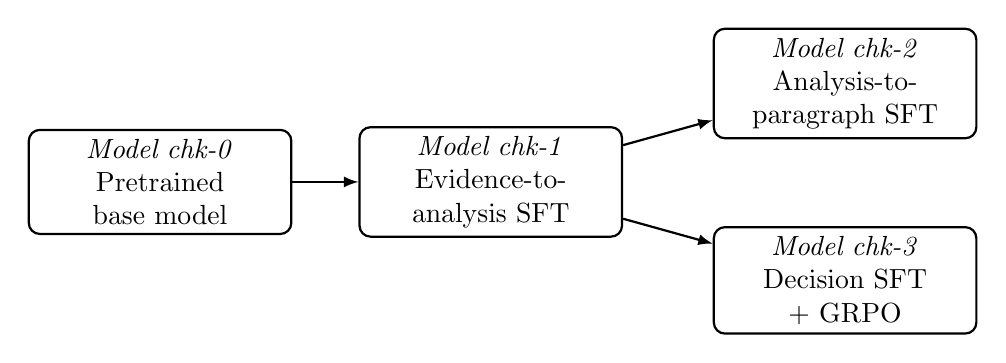
\begin{tikzpicture}[
        >=latex,
        model/.style={draw, rounded corners, align=center, text width=3.1cm,
            minimum height=1.25cm},
        every path/.style={->, thick}
    ]
        \node[model] (chk0) at (0,0)
            {\textit{Model chk-0}\\Pretrained base model};
        \node[model] (chk1) at (4.2,0)
            {\textit{Model chk-1}\\Evidence-to-analysis SFT};
        \node[model] (chk2) at (8.7,1.25)
            {\textit{Model chk-2}\\Analysis-to-paragraph SFT};
        \node[model] (chk3) at (8.7,-1.25)
            {\textit{Model chk-3}\\Decision SFT + GRPO};
        \draw (chk0) -- (chk1);
        \draw (chk1) -- (chk2);
        \draw (chk1) -- (chk3);
    \end{tikzpicture}
    \caption{Final paper-level training lineage.}
    \label{fig:ch2:training_stage1}
\end{figure}

Figure~\ref{fig:ch2:training_process} expands the lineage into the data and
optimization flows for analytical SFT and the two downstream tasks. The
retained diagrams use the original experimental identifiers: the
\textit{Model chk-3} and \textit{Model chk-4} labels printed in the graphics
correspond, respectively, to the paper-level \textit{Model chk-2} and
\textit{Model chk-3}. In addition, the ``Minutes'' box in the decision panel is
an earlier project-side shorthand; the finalized decision model receives the
target-neutral, pre-meeting analysis specified later in this section.

\begin{figure}[H]
    \centering
    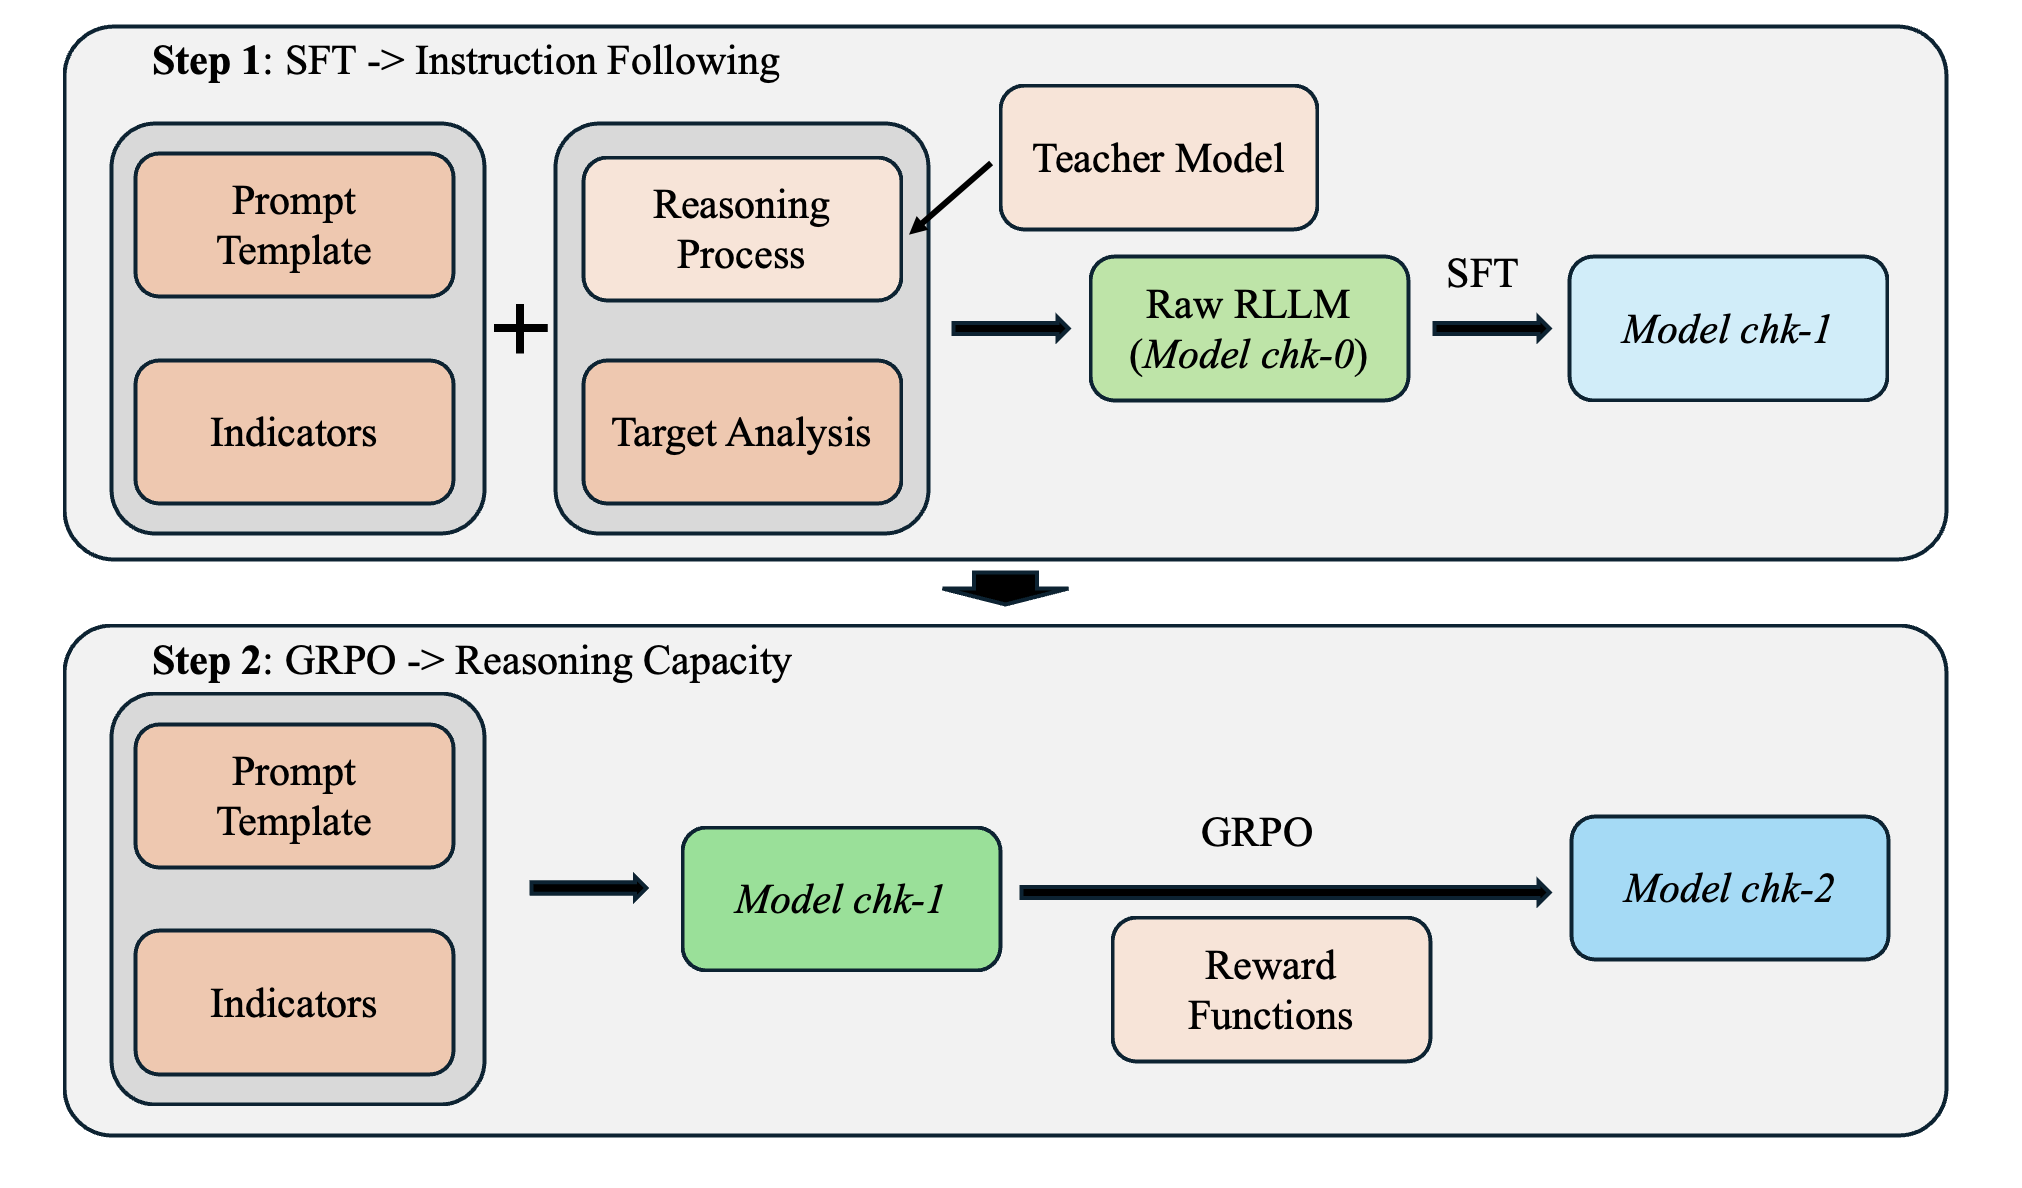
\includegraphics[width=\textwidth]{train/stage1.png}
    \par\medskip
    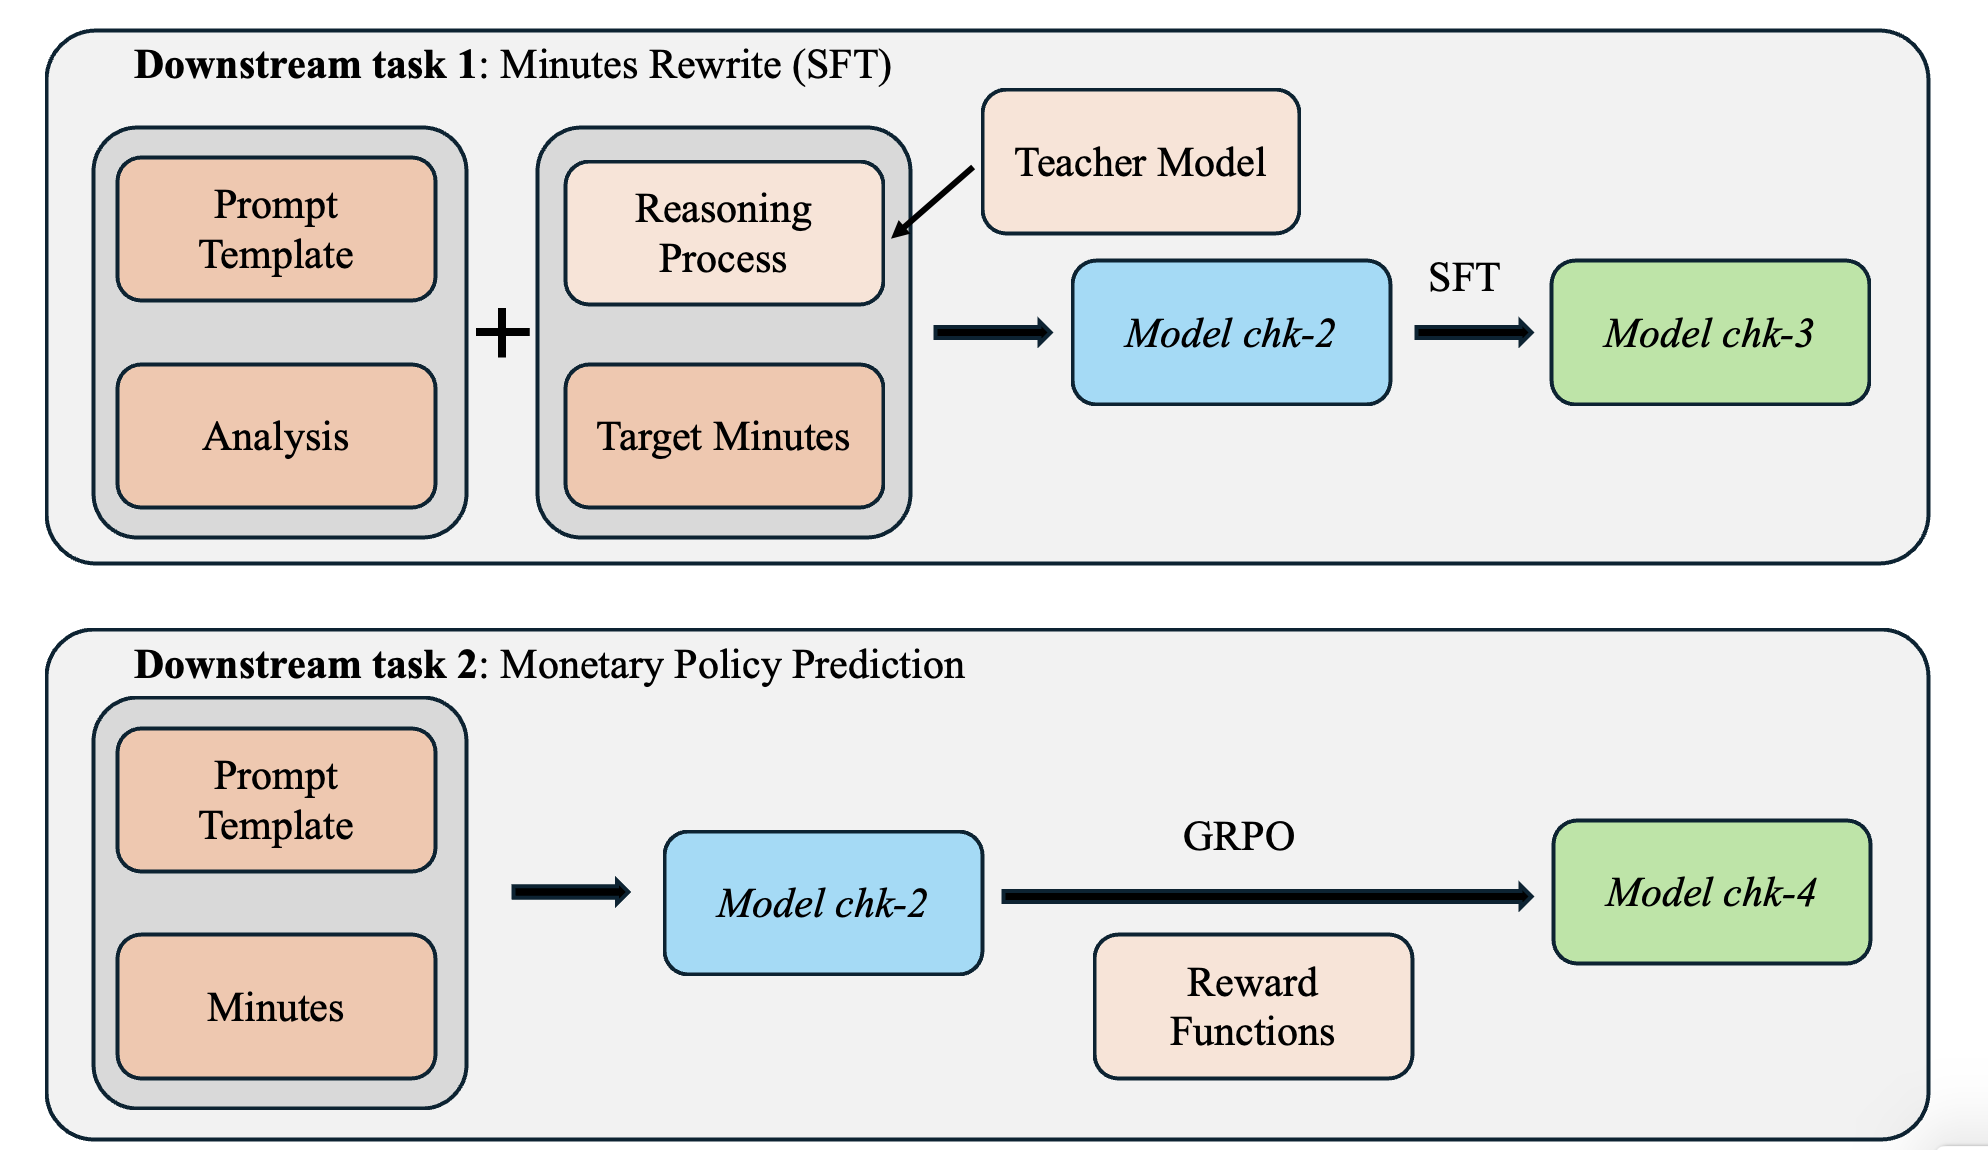
\includegraphics[width=\textwidth]{train/stage2.png}
    \caption{Overview of Two-step Training Process}
    \label{fig:ch2:training_process}
\end{figure}


%SFT
\paragraph*{Supervised fine-tuning.}
SFT adapts the model to the macro-financial tasks by learning from paired
prompts and reference completions. Each training example contains a system
instruction, a user prompt, and a target assistant response. The model is
optimized under teacher forcing, while parameter-efficient adapters reduce
the number of trainable parameters. Figure~\ref{fig:ch2:ft_detail} summarizes
this workflow.


\begin{figure}
    \begin{center}
        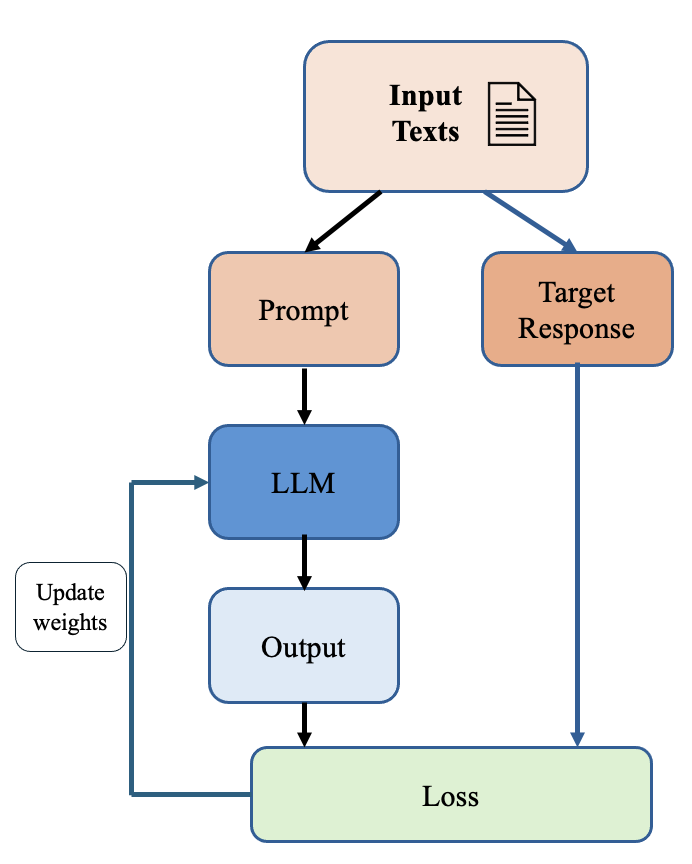
\includegraphics[width=0.3\textwidth]{Chapter2/Chapter2Figs/ft_detail.png}
      \end{center}
      \caption{Supervised fine-tuning workflow.}
      \label{fig:ch2:ft_detail}
\end{figure}



During SFT, let $x=(x_1,\ldots,x_M)$ denote the serialized prompt and
$y=(y_1,\ldots,y_N)$ the target assistant completion. At each target
position, the model predicts a distribution over the vocabulary conditional
on the prompt and preceding target tokens. The mean token-level negative
log-likelihood is
\begin{equation}
    \mathcal{L}_{\mathrm{SFT}}(\theta)
    =
    -\frac{1}{W}
    \sum_{t=1}^{N}
    w_t
    \log \pi_\theta\!\left(y_t\mid x,y_{<t}\right),
    \qquad
    W=\sum_{t=1}^{N}w_t,
\end{equation}
where $w_t\in\{0,1\}$ masks padding and any positions excluded from the
supervised objective. If every completion token is trained, $w_t=1$ and
$W=N$. Thus, SFT minimizes the negative log-probability assigned to the
reference completion; it does not compare a separately decoded response with
the target text.


%RL
\paragraph*{Reinforcement learning.}
Unlike SFT, policy optimization does not require a token-level reference
completion. In the decision task, however, the reference action remains
available to the deterministic reward function: the policy sees the prompt,
whereas the target direction and magnitude are used only to score sampled
completions.

Proximal Policy Optimization (PPO; \cite{schulman2017proximal}) stabilizes
policy-gradient updates by clipping the importance-sampling ratio. Let
$s_t=(q,o_{<t})$ be the token-generation state and define
\begin{equation*}
    \rho_t(\theta)
    =
    \frac{\pi_\theta(o_t\mid s_t)}
         {\pi_{\theta_{\mathrm{old}}}(o_t\mid s_t)}.
\end{equation*}
The clipped policy objective is
\begin{equation}
    \mathcal{J}_{\mathrm{PPO}}(\theta)
    =
    \mathbb{E}_t\!\left[
        \min\!\left(
            \rho_t(\theta)\widehat{A}_t,
            \operatorname{clip}
            \bigl(\rho_t(\theta),1-\epsilon,1+\epsilon\bigr)
            \widehat{A}_t
        \right)
    \right].
\end{equation}
Here, $\widehat{A}_t$ is an advantage estimate rather than the reward itself;
clipping constrains the policy ratio rather than rescaling the reward.




GRPO (\cite{shao2024deepseekmath}) removes the learned value function. For
each prompt $q$, the behavior policy samples a group
$\{o_i\}_{i=1}^{G}$, and the task reward assigns one terminal score
$R_i=R(q,y,o_i)$ to each completion. The group-relative advantage is
\begin{equation}
    \widehat{A}_i
    =
    \begin{cases}
    \displaystyle\frac{R_i-\overline{R}}{s_R+\eta}, & s_R>0,\\[7pt]
    0, & s_R=0,
    \end{cases}
    \qquad
    \overline{R}=\frac{1}{G}\sum_{j=1}^{G}R_j,
\end{equation}
where $s_R$ is the within-group reward standard deviation and $\eta>0$ is a
numerical stabilizer. The same completion-level advantage is applied to every
generated token in $o_i$. A group whose completions all receive the same
reward therefore supplies no group-relative learning signal.




For token $t$ of completion $i$, define
\begin{equation*}
    \rho_{i,t}(\theta)
    =
    \frac{\pi_\theta(o_{i,t}\mid q,o_{i,<t})}
         {\pi_{\theta_{\mathrm{old}}}(o_{i,t}\mid q,o_{i,<t})}.
\end{equation*}
A sampled per-token estimator for the KL regularizer is
\begin{equation*}
    \widehat{D}_{\mathrm{KL},i,t}
    =
    \frac{\pi_{\mathrm{ref}}(o_{i,t}\mid q,o_{i,<t})}
         {\pi_\theta(o_{i,t}\mid q,o_{i,<t})}
    -\log
    \frac{\pi_{\mathrm{ref}}(o_{i,t}\mid q,o_{i,<t})}
         {\pi_\theta(o_{i,t}\mid q,o_{i,<t})}
    -1.
\end{equation*}
Using
\begin{equation*}
    \ell_{i,t}(\theta)
    =
    \min\!\left(
        \rho_{i,t}(\theta)\widehat{A}_i,
        \operatorname{clip}
        \bigl(\rho_{i,t}(\theta),1-\epsilon,1+\epsilon\bigr)
        \widehat{A}_i
    \right)
    -\beta\widehat{D}_{\mathrm{KL},i,t},
\end{equation*}
the original sequence-normalized GRPO objective can be written as
\begin{equation}
    \mathcal{J}_{\mathrm{GRPO}}(\theta)
    =
    \mathbb{E}\!\left[
        \frac{1}{G}\sum_{i=1}^{G}
        \frac{1}{|o_i|}\sum_{t=1}^{|o_i|}
        \ell_{i,t}(\theta)
    \right].
\end{equation}

The completed decision run instead sets \texttt{loss\_type=dapo}. In this
trainer setting, DAPO denotes token-level loss aggregation: the losses are
normalized by the number of active completion tokens in the accumulated
training batch rather than separately by each completion length. If
$\mathcal{C}$ is the set of unmasked completions in that batch, the realized
aggregation is
\begin{equation}
    \mathcal{J}_{\mathrm{DAPO}}(\theta)
    =
    \mathbb{E}\!\left[
        \frac{\displaystyle
            \sum_{i\in\mathcal{C}}\sum_{t=1}^{|o_i|}\ell_{i,t}(\theta)}
             {\displaystyle
            \sum_{i\in\mathcal{C}}|o_i|}
    \right].
\end{equation}
This setting is related to the token-level aggregation proposed in DAPO
(\cite{yu2025dapo}), but it does not imply that the run adopted the complete
DAPO recipe. The realized configuration retained symmetric clipping and a KL
penalty; its numerical settings are reported with the decision-training
configuration below.





\subsection*{Analytical and Downstream Training}

\subsubsection*{Supervised Fine-tuning for the Analytical Model}

\paragraph*{Model chk-1.}
The first SFT stage adapts \textit{Model chk-0} to point-in-time
macro-financial analysis. Each supervised example is a pair
$(q_i,o_i^{\mathrm{SFT}})$, where $q_i$ is the model-visible prompt and
$o_i^{\mathrm{SFT}}=(c_i,a_i)$ is the reference assistant completion. Here,
$c_i$ denotes the reasoning prefix and $a_i$ the concise final analysis. This
distinction separates the model input from the supervision target. Training
for a small number of epochs limits, but does not eliminate, the risk that the
model memorizes task-specific wording.



Moreover, each LLM requires a model-specific message format, because tokenizers encode role boundaries differently. Explicit role labels are used specifically to distinguish the sections: the ``\texttt{System Prompt}'', ``\texttt{User Prompt}'', and ``\texttt{Assistant Response}''. Table. \ref{tab:ch2:input_template_for_llama3} presents the labels used by LLAMA3, where ``\prompttag{start\_header\_id}'' and ``\prompttag{end\_header\_id}'' wrap around the role labels indicating the message type. The label ``\prompttag{begin\_of\_text}'' signals the start of the conversation, while ``\prompttag{end\_id}'' denotes its end.



\begin{table}[h]
    \centering
    \footnotesize
    \begin{tabular}{p{0.98\textwidth}}
    \toprule
    \textbf{Special Labels for LLaMA 3:} \\
    \midrule
    \prompttag{begin\_of\_text} \\
    \prompttag{start\_header\_id} \textcolor{red}{system}\prompttag{end\_header\_id} \\
    \texttt{... System Prompts ...} \\
    \prompttag{start\_header\_id} \textcolor{red}{user}\prompttag{end\_header\_id} \\
    \texttt{... User Prompts ...} \\
    \prompttag{start\_header\_id} \textcolor{red}{assistant}\prompttag{end\_header\_id} \\
    \texttt{... Assistant Response ...} \\
    \prompttag{end\_id} \\
    \bottomrule
    \end{tabular}
    \caption{Input Template for LLAMA3}
    \label{tab:ch2:input_template_for_llama3}
\end{table}



\paragraph*{Reasoning boundary and final answer.}
The supervised completions follow the model's native reasoning-boundary
convention. A nonempty reasoning prefix $c_i$ is followed by exactly one
literal \texttt{</think>} marker and a nonempty final
answer $a_i$. Writing the boundary token as $b_{\mathrm{think}}$, the
serialized completion is
\begin{equation*}
    o_i=c_i\;\Vert\;b_{\mathrm{think}}\;\Vert\;a_i,
\end{equation*}
where $\Vert$ denotes string concatenation,$b_{\mathrm{think}} = \texttt{</think>} $. The semantic form of $a_i$ is task-specific: prose for \textit{Models chk-1} and \textit{chk-2}, and a decision object for \textit{Model chk-3}. 






\subsubsection*{Further Training for Downstream Tasks}

We adapt \textit{Model chk-1} separately for two downstream tasks. SFT on
analysis-to-FOMC-Minutes-style paragraph pairs produces \textit{Model chk-2}.
A separate branch uses decision SFT followed by GRPO to produce
\textit{Model chk-3}, which
predicts the direction and magnitude of a federal funds rate action.


\paragraph*{FOMC-Minutes-Style Paragraph Rewriting (\textit{Model chk-2})}

The Minutes-rewriting branch begins from the exact-merged \textit{Model chk-1}  and applies task-specific supervised fine-tuning to learn an analysis-to-paragraph transformation. 

First of all, because official FOMC Minutes often contain substantial details absent from the corresponding economic-analysis passages used as training inputs, treating the Minutes directly as targets would create misaligned supervision. We therefore used a teacher model to reconstruct a factually complete, de-styled analysis from each Official Minutes paragraph, ensuring that the student learns stylistic rewriting rather than supplying missing facts.

Then, for each training instance, the student model receives a fixed system instruction and a user message containing the analysis to be rewritten. Under teacher forcing, the target completion consists of a fidelity-planning reasoning section, one literal \texttt{</think>} boundary, and a single rewrote formal FOMC Minutes paragraph. The optimization objective therefore emphasizes the preservation of claims, quantities, dates, directions, comparisons, and uncertainty while adapting the output to the institutional style and structure of the FOMC Minutes. 




\paragraph*{Monetary Policy Decision Making (\textit{Model chk-3})}

The monetary-policy decision branch begins independently from the exact-merged \textit{Model chk-1} and proceeds through decision-specific SFT followed by GRPO. During SFT, the model receives a fixed system instruction and a user message containing a target-neutral pre-meeting analysis. The supervised completion consists of a qualitative dual-mandate rationale, one literal \texttt{</think>} boundary, and a terminal object specifying the policy direction and magnitude. GRPO then initializes from decision SFT checkpoint, retains the same model-facing prompt, action space, and response contract, and optimizes the parser-contingent decision proxy reward. 



\subsection*{Technique for Parameter-Efficient Fine-Tuning (PEFT)}

Full-parameter fine-tuning updates every model parameter and must retain the
associated gradients and optimizer states. Parameter-efficient fine-tuning
instead freezes the pretrained weights and optimizes a much smaller set of
task-specific parameters.

We use Low-Rank Adaptation (LoRA; \cite{hu2021lora}). For a pretrained linear
transformation with weight
$W\in\mathbb{R}^{d_{\mathrm{out}}\times d_{\mathrm{in}}}$, LoRA represents
the trainable update as
\begin{equation}
    W'=W+\Delta W,
    \qquad
    \Delta W=\frac{\alpha}{r}BA,
\end{equation}
where $A\in\mathbb{R}^{r\times d_{\mathrm{in}}}$,
$B\in\mathbb{R}^{d_{\mathrm{out}}\times r}$, and
$r\ll\min(d_{\mathrm{in}},d_{\mathrm{out}})$. The pretrained matrix $W$
remains frozen; only the low-rank factors are optimized.

Quantized Low-Rank Adaptation (QLoRA; \cite{dettmers2024qlora}) combines LoRA
with a quantized frozen base model; its 4-bit NormalFloat (NF4) representation
is distinct from generic FP4. The final training record for \textit{chk-2}
checkpoint 50 verifies NF4 QLoRA training with double quantization and
BF16 compute and storage, using a rank-32, $\alpha=64$ LoRA adapter with
dropout 0.05 on \texttt{q\_proj},
\texttt{k\_proj}, \texttt{v\_proj}, \texttt{o\_proj},
\texttt{gate\_proj}, \texttt{up\_proj}, and \texttt{down\_proj}. The main
text-similarity evaluation loads this adapter over the exact-merged
\textit{chk-1} checkpoint 200 parent in BF16 without inference quantization;
the \textit{chk-2} adapter itself remains active rather than being merged.
An adapter may remain
separate from its parent model or be merged for deployment; merging does not
by itself reduce the size of the resulting base-sized model.




\subsection{Training Hyperparameters}\label{ch2:sec:parameter}

Table~\ref{tab:ch2:training_hyperparameters_archive} reports checkpoint
identities and configuration values. 

\begin{table}[H]
    \centering
    \footnotesize
    \setlength{\tabcolsep}{3pt}
    \renewcommand{\arraystretch}{1.16}
    \begin{tabularx}{\textwidth}{@{}
        >{\centering\arraybackslash}p{0.08\textwidth}
        >{\centering\arraybackslash}p{0.08\textwidth}
        >{\raggedright\arraybackslash}p{0.18\textwidth}
        >{\raggedright\arraybackslash}p{0.18\textwidth}
        >{\raggedright\arraybackslash}X
    @{}}
        \toprule
        \textbf{Model} & \textbf{Stage} & \textbf{Initialization} &
        \textbf{Selected Point} &
        \textbf{Configuration} \\
        \midrule
        \textit{chk-1} & SFT & \textit{chk-0} & Checkpoint 200 selected and
        exact-merged & Final evaluation records fix the artifact identity;
        full training settings are not bound in the current record set. \\
        \textit{chk-2} & SFT & Exact-merged \textit{chk-1} checkpoint 200 &
        Checkpoint 50 selected by the validation-probe rule; active adapter &
        NF4 QLoRA $r=32$, $\alpha=64$, dropout 0.05; learning rate
        $10^{-6}$; three epochs (60 optimizer steps); completion-only loss.
        Selection evidence is reported in Appendix~\ref{app:checkpoint_selection}. \\
        \textit{chk-3} & SFT & Exact-merged \textit{chk-1} checkpoint 200 &
        Checkpoint 38 initializes GRPO & 211 unique meetings, 312 physical
        training rows. \\
        \textit{chk-3} & GRPO & Decision SFT checkpoint 38 & Run completed at
        step 468; checkpoint 450 used for evaluation &
        \texttt{loss\_type=dapo}; within-group scaling; four generations per
        prompt; generation batch 8; temperature 0.7; top-$p$ 0.9;
        $\beta=0.04$; $\epsilon=0.2$; prompt/completion limits 2,560/1,536;
        truncated completions masked; sole proxy reward
        \texttt{decision\_dense\_v3} with external weight 1.0. \\
        \bottomrule
    \end{tabularx}
    \caption{Paper-level model lineage and verified subset of the training configuration.}
    \label{tab:ch2:training_hyperparameters_archive}
\end{table}





\section{Model Evaluation Methods}\label{ch2:sec:application}


In this section, we evaluate the fine-tuned LLM's outputs with a focus on reliability. Given that LLMs are probabilistic generators, which selects the next token based on the highest probability, a critical issue encountered is the phenomenon known as hallucination. Hallucination refers to instances where the content generated by the model is unsupported by or conflicts with factual information. \cite{huang2025survey} have identified two primary forms of hallucination in LLMs: factuality hallucination and faithfulness hallucination. Factuality hallucination occurs when generated content contradicts real-world facts, whereas faithfulness hallucination arises when the generated content does not align consistently with the provided input. Consequently, tests designed to detect hallucinations are essential for evaluating the reliability of LLMs.




% LLM evaluation can be broadly classified as reference-based or reference-free. Reference-based evaluation compares model outputs with frozen targets under the same prompts; examples include string-overlap measures such as BLEU \cite{papineni2002bleu} and embedding-based measures such as BERTScore \cite{zhang2019bertscore}. Reference-free evaluation instead examines outputs without a target text, for example through econometric diagnostics, expert assessment, or a separately specified model-based evaluator.

LLM evaluation can be broadly classified into reference-based and reference-free evaluation. First, reference-based evaluation compares the model’s outputs with target outputs generated under the same prompts. Scores are then used to quantitatively measure the differences between them. For instance, the F1 score measures classification accuracy, BLEU \cite{papineni2002bleu} measures string-level overlap, and BERTScore \cite{zhang2019bertscore} measures semantic similarity based on token embeddings. Notably, reference outputs are required for reference-based evaluation. By contrast, reference-free evaluation does not require predefined target outputs. It is usually model-based or judgement-based, including regression-based validation between input prompts and outputs, LLM-as-Judge scoring, and human assessment.


Because high-quality reference answers are available in this study, we primarily use reference-based evaluation. More specifically, we will evaluate the fine-tuned model across four key dimensions:  1) the \textbf{textual similarity} of generated outputs, 2) the \textbf{sufficiency of information} contained in the outputs, 3) the \textbf{statistical significance} of synthetic text, 4) the \textbf{accuracy of simulated decision-making}. 

First, we compare generated paragraphs with teacher-generated synthetic rewriting references on the 391-row, 124-meeting release described in Section~\ref{ch2:sec:the-dataset}. This measures reconstruction similarity within a training-only release, not performance against official Minutes or on an independent test set. Second, the separate historical Core8 sensitivity analysis and sentiment diagnostics examine topic dependence and policy-stance alignment. Third, the financial-market diagnostic compares coefficients estimated from generated texts with those estimated from official Minutes. Finally, simulated decision-making accuracy is evaluated separately through the Model chk-3 decision branch using direction accuracy, balanced accuracy, macro-F1, exact-action accuracy, and delivery measures.


The first two dimensions describe semantic resemblance and sensitivity to
supplied prompt blocks. Neither metric directly verifies factual preservation
or detects unsupported claims; those properties require separate fidelity
audits. The financial-market and decision dimensions provide historical
association and policy-action diagnostics, respectively, with their own
evaluation populations and limits.




\subsection*{Evaluation Methods}


\subsubsection*{Textual Similarity of Minutes-Style Paragraph-Rewriting}


To start with, the textual similarity targets comparing the similarity between the target output and the generated output using mathematical distance, such as the Levenshtein Similarity Ratio (\cite{levenshtein1966binary}) and Cosine Similarity (\cite{tanguy2016natural}). The Levenshtein Similarity Ratio replies on the Levenshtein Distance to measure the minimum number of strings that need to be edited from the generated output to the required output. Furthermore, some other metrics driven from the idea of ``n-grams'', such as the Recall-Oriented Understudy for Gisting Evaluation score (ROGUE score, \cite{lin2004rouge}), provide an grammatical-level measurement than the word-level Levenshtein Similarity Ratio. These methods are useful at the age of ``Bag-Of-Word (BOG)''.


However, with the development of LLM, researchers can take advantage of the embeddings from the LLM rather than the one-hot key of ``BOG''. The embeddings can convert the ``word'' into tokens that encoded more semantic information than the one-hot key. 


Therefore, the Cosine Similarity provides a more accurate estimation of the semantic similarity between two texts. Here, we will use the \textit{sentence-level} \textbf{Cosine Similarity} as our first metric to evaluate the text similarity of outputs. Cosine Similarity ranges from 0 to 1, where a value of 1 indicates a perfect similarity between the two texts, while a value of 0 signifies that the texts are highly different from each other.


The metric helps in determining how well the generated text aligns with the expected content in terms of both meaning and context. For example, \cite{aynetdinov2024semscore}, \cite{kim2024comparison}, and \cite{yauney2023data} used the Cosine Similarity as a benchmark when evaluating the LLM's performance.

Cosine similarity is estimated by the cosine of the angle between two non-zero vectors. It is defined as the dot product of the two vectors divided by the product of their magnitudes. This mathematical operation helps in quantifying how closely the generated text aligns with the target text in terms of meaning and content. We utilize the ``tokenizer'' and the ``hidden layers'' from the LLAMA3 model to convert the response texts into vector representations, denoted as $Y$ for the target text and $\hat{Y}$ for the generated text. Then, the cosine similarity score, denoted as $Cos_{Y, \hat{Y}}$, is then calculated as follows:



\begin{equation*}
    Cos_{Y, \hat{Y}} = \frac{Y \cdot \hat{Y}}{\|Y\|_2 \|\hat{Y}\|_2}
\end{equation*}

where $Y$ and $\hat{Y}$ are sentence embeddings for the reference and generated texts, and $\|\cdot\|_2$ denotes the Euclidean norm (e.g., $\|Y\|_2=\sqrt{y_1^2+y_2^2+\cdots+y_N^2}$).


% According to the distribution theory, 
Finally, drawing from distributional semantics theory (\cite{firth1957linguistics}, \cite{sahlgren2008distributional}), words with similar meanings tend to occur in similar contexts and thus have similar distributions in the vector space. Therefore, we hypothesize that texts with higher semantic likeness will exhibit a greater cosine similarity. 


% BERTScore 

On the other hand, in addition to Cosine Similarity, which serves as a \textit{sentence-level} metric, we also employ \textbf{BERTScore} (\cite{zhang2019bertscore}), a metric designed to capture \textit{token-level} semantic similarity using cosine similarity as its underlying distance measure.

More specifically, for each token $\hat{y}_j$ in the target (reference) output $\hat{Y}$, BERTScore identifies the maximum cosine similarity with respect to all candidate tokens $y_i$ in the generated response $Y$. These maximal token-level similarities are then aggregated to construct three complementary evaluation metrics: \textit{Recall} ($BertScore^{Recall}$), \textit{Precision} ($BertScore^{Precision}$), and the harmonic mean of the two, the \textit{F1 score} ($BertScore^{F1}$).


Let $Y=\{y_i\}$ denote the set of token embeddings in the generated response and $\hat{Y}=\{\hat{y}_j\}$ denote the set of token embeddings in the reference (target) text. BERTScore computes \textit{Precision} by matching each candidate token to its most similar reference token, and \textit{Recall} by matching each reference token to its most similar candidate token. Finally, the F1 Score (Eq.(\ref{eq:ch2:bert_f1})) is calculated as the harmonic mean of precision and recall, thereby providing a balanced measure of semantic alignment between the generated and reference texts:


\begin{equation}\label{eq:ch2:bert_precision}
    BERTScore^{Precision} = \frac{1}{\|Y\|}\sum_{y_i \in Y} \max_{\hat{y}_j \in \hat{Y}} y_i^{\text{T}}\hat{y}_j
\end{equation}

\begin{equation}\label{eq:ch2:bert_recall}
    BERTScore^{Recall} = \frac{1}{\|\hat{Y}\|}\sum_{\hat{y}_j \in \hat{Y}} \max_{y_i \in Y} \hat{y}_j^{\text{T}}y_i
\end{equation}

\begin{equation}\label{eq:ch2:bert_f1}
    BERTScore^{F1} = \frac{2\cdot BERTScore^{Precision}\cdot BERTScore^{Recall}}{BERTScore^{Precision}+BERTScore^{Recall}}
\end{equation}


Overall, we propose the following hypotheses for cosine similarity and BERTScore-F1:

\begin{equation*}
    \begin{split}
        &Cos_{FT} - Cos_{Base} > 0 \\
        &BERTScore^{F1}_{FT} - BERTScore^{F1}_{Base} > 0
    \end{split}
\end{equation*}


where subscripts $FT$ and $Base$ denote the fine-tuned and baseline models. The hypothesis is that fine-tuning increases semantic alignment with the target text. For the main rewriting comparison, we average raw-best-effort scores over the ten generations of each sample and then over samples within each meeting. The 124 meetings receive equal weight. Table~\ref{tab:ch2:minutes_semantic_ttest} reports supplementary, unadjusted two-sided paired $t$-tests of these meeting means; the frozen experiment's hierarchical paired-bootstrap intervals are reported separately in the results. A positive paired difference indicates greater resemblance to the synthetic target under this scoring rule. It does not identify additional macroeconomic knowledge, factual fidelity, or held-out generalization.


%%%%% end of text similarity


\subsubsection*{Sufficient Information}

Apart from textual similarity, we also require the generated output to reflect information supplied by the input indicators rather than relying solely on unsupported completion. The question in this subsection is therefore not only whether the generated section resembles the target text, but also whether removing a given indicator materially changes that resemblance.


To study this issue, our second metric evaluates the marginal informational contribution of each indicator prompt to the generated output. Shapley-style attribution methods provide the relevant conceptual background because they quantify how much each input contributes to an observed output. Originating in cooperative game theory, the Shapley Value (\cite{shapley1953value}) measures the expected marginal contribution of one player to a coalition. This idea has since been adapted to model interpretation, including Shapley Regression Value (\cite{lipovetsky2001analysis}), Shapley Sampling Value (\cite{vstrumbelj2014explaining}), Quantitative Input Influence (\cite{datta2016algorithmic}), Shapley Additive Explanations (\cite{lundberg2017unified}), and token-level attribution methods such as TokenShapley (\cite{liu2023prompt}; \cite{mohammadi2024wait}; \cite{goldshmidt2024tokenshap}).




As literature background, the original Shapley Value ($\mathcal{SV}$) represents the expected marginal contribution of a feature ($p_i$) to a model output $f(\cdot)$:

\begin{equation*}
  \mathcal{SV}_i(f) = \sum_{\mathcal{S} \subset \mathcal{P}\setminus p_i} \frac{\left|\mathcal{S}\right|! (n - \left|\mathcal{S}\right| - 1)!}{n!} \left(f(\mathcal{S}\cup p_i) - f(\mathcal{S})\right)
\end{equation*}

where $\mathcal{P}=\{p_1, p_2, \cdots, p_n\}$ is the set of prompts, $\mathcal{S}$ is a coalition (subset) of prompts, and $f(\cdot)$ is a utility function. The term $f(\mathcal{S}\cup p_i)-f(\mathcal{S})$ denotes the marginal contribution of feature $p_i$ to coalition $\mathcal{S}$.


In this research, however, we do not estimate the full Shapley Value across all possible coalitions. Instead, we adopt a \textbf{Shapley-inspired, indicator-level leave-one-out (LOO) masking test} (Leave-one-out test hereafter). The purpose is the same in spirit: to measure how much each indicator matters for the generated section. 


More, specifically, we choose 8 core topics, including the Consumer Price Index (CPI), GDP Growth, Government Purchases, Housing Starts, Industrial Production, the Labour Market, Money Supply, and the Unemployment Rate, in this test. For metric \(m\), the leave-one-out (LOO) effect is defined as 

\begin{equation}\label{eq:ch2:loo}
    \delta^{(m)}_{h,r,a,t}=S^{(m)}(O^{\mathrm{Full}}_{h,r},R_h)-S^{(m)}(O^{(a,t)}_{h,r},R_h), 
\end{equation}


where \(R_h\) denotes the same complete deterministic synthetic reference for meeting \(h\), \(a\) denotes either exact deletion or token-matched neutral replacement, \(t\) identifies the intervened topic, and \(m\) denotes either cosine similarity or BERTScore-F1. A positive value of \(\delta\) indicates that deleting or neutralizing the topic reduces the output’s similarity to the common reference, whereas a negative value indicates that the intervention produces an output that is more similar to the reference. A confidence interval that crosses zero indicates that the analysis does not establish a directionally stable aggregate change under the specified intervention and evaluation design.




%%%% end of Core8 LOO sensitivity diagnostic


\subsubsection*{Statistical Significance using Synthetic Texts}


This test evaluates the model’s simulation capacity by conducting empirical analyses on the synthetic text it generates. The current literature has confirmed the impact of the release of FOMC Minutes on the financial market, for instance, \cite{rosa2013financial} found that the release of the Minutes significantly increases the volatility of the U.S. asset prices, including treasury rate, equity market index and the exchange rate. \cite{rosa2011high} found that both the statements and the policy decisions have significant effects on the exchange rate market. \cite{huang2021economic} applied an adaptive Bayesian text mining approach, and confirmed the predictive power of the sentiments of FOMC's text in important economic variables. \cite{tadle2022fomc} confirmed the sentiments contained in the Minutes have significantly impacts on the fed funds futures rate and U.S. dollars exchange rate.


Building on these evidences, we test whether the synthetic Minutes generated by our fine-tuned LLM exhibit comparable market relevance. Specifically, a statistically significant relationship between the synthetic text and corresponding financial indicators would indicate that the model is capable of producing realistic, policy-relevant content that mirrors the economic impact of actual FOMC communications.


We adapt the empirical framework of \citet{tadle2022fomc}. Tadle relates unexpected sentiment in FOMC communications to changes in financial-market variables, including Federal Funds futures and exchange rates. In our application, the main regression model Eq.~\ref{eq:ch2:tadle_ff_regression} is estimated separately using sentiment measures derived from official Minutes and from each generated-text checkpoints. We are expecting our synthetic minutes yields similar effects on financial market variables. Finally, We estimate the following specification for Federal Funds futures returns:


\begin{equation}
\label{eq:ch2:tadle_ff_regression}
\begin{aligned}
r_t^f
={}&
\alpha
+\beta_{\mathrm{NS}}NS_t
+\beta_{\ell_{2011}\times\mathrm{NS}}
 \left(\ell_{2011,t}\times NS_t\right) \\
&+\beta_{\mathrm{VIX}}VIX_t
+\beta_{\ell_{2011}}\ell_{2011,t}
+\boldsymbol{\beta}_{Y}^{\prime}\mathbf{Y}_t
+\phi_t ,
\end{aligned}
\end{equation}

where the dependent variable is the daily log-percentage change in the price of the Federal Funds futures contract at horizon
\(f\in\{1,3,6,12\}\):

\begin{equation}
\label{eq:ch2:ff_return}
r_t^f
=
100\left(\ln P_t^f-\ln P_{t-1}^f\right)
=
100\ln\left(\frac{P_t^f}{P_{t-1}^f}\right).
\end{equation}

The indicator for the date-based forward-guidance regime is defined as

\begin{equation}
\label{eq:ch2:post2011_indicator}
\ell_{2011,t}
=
\begin{cases}
1, & t>\text{8 August 2011},\\
0, & \text{otherwise}.
\end{cases}
\end{equation}

The variable \(VIX_t\) is the daily log-percentage change in the
adjusted closing value of the CBOE Volatility Index, vector \(\mathbf{Y}_t\) is calendar-year fixed effect, and \(\phi_t\) denotes the regression error. The coefficient \(\beta_{\mathrm{NS}}\) measures the association between the Minutes news shock and the futures return before the date-based forward-guidance regime, whereas \(\beta_{\ell_{2011}\times\mathrm{NS}}\) measures the change in this association after the regime begins. The corresponding post-2011 marginal coefficient is therefore


\begin{equation}
\label{eq:ch2:post2011_marginal_beta}
\beta_{\mathrm{post}}
=
\beta_{\mathrm{NS}}
+
\beta_{\ell_{2011}\times\mathrm{NS}}.
\end{equation}

The Minutes news shock is constructed in two stages. First, relative sentiment is defined as the difference between the standardized Minutes and Statement sentiment scores, which are measured using the Loughran--McDonald dictionary \citep{loughran2011liability}:

\begin{equation}
\label{eq:ch2:relative_sentiment}
RZ_t
=
Z_t^M-Z_t^S,
\end{equation}

where \(Z_t^M\) and \(Z_t^S\) denote the standardized sentiment scores of the Minutes and the corresponding FOMC Statement, respectively. Second, the predictable component of relative sentiment is removed:

\begin{equation}
\label{eq:ch2:minutes_news_shock}
NS_t
=
RZ_t-0.368RZ_{t-1}.
\end{equation}

Thus, \(NS_{m,t}\) measures the source-specific component of relative sentiment not captured by its immediately preceding value. The constructed news-shock
regressor is not subsequently standardized to unit variance.


We conduct the test with the generated minutes by \textit{Model chk-0}, \textit{Model chk-1}, and \textit{Model chk-2}. Then, we calculated the distance  between the synthetic texts' coefficients ($\beta_{\mathrm{chk-0, chk-1, chk-2}}$) with that of the official Minutes ($\beta_{O}$):

\begin{equation}
\label{eq:ch2:tadle_beta_distance}
D_{m,O}
=
\left|
\widehat{\beta}_{m,\mathrm{post}}
-
\widehat{\beta}_{O,\mathrm{post}}
\right|,
\qquad m\in\{0,1,2\},
\end{equation}

and define the direct \textit{Model chk-2} distance gain relative to comparator
\(j\in\{0,1\}\) as

\begin{equation}
\label{eq:ch2:tadle_beta_gain}
G_j=D_{j,O}-D_{2,O}.
\end{equation}


Following the empirical test, we conduct a bootstrap procedure to estimate the distribution of the $\beta$ coefficients. A statistically significant positive gain means that the model $m$ is closer to the official coefficient at that horizon. 




%%%% end of sentiment-score closeness and historical Federal Funds futures diagnostic


\subsubsection*{Decision-making Accuracy}

Finally, at each Federal Open Market Committee (FOMC) meeting, the Committee votes on monetary policy decisions—most notably the target range of the Federal Funds Rate (FFR), also referred to as the Federal Funds Target Rate. Once the target rate is established, the Federal Reserve employs a range of monetary policy instruments to steer the effective FFR toward the desired level by adjusting the supply of reserves within the banking system. These instruments include open market operations (purchasing and selling U.S. government securities), the Interest on Reserve Balances (IOR), and the Overnight Reverse Repurchase Agreement (ON RRP) facility. Consequently, FOMC decisions exert a direct influence on the interest rate market, with subsequent spillover effects on exchange rates and equity markets.


The final stage of our empirical evaluation assesses the model’s simulation ability to predict monetary policy decisions, specifically changes in the Federal Funds Rate, based on macroeconomic and financial indicators. In this context, each FOMC meeting represents a decision-making instance in which the Committee determines the appropriate policy stance in response to evolving economic conditions and market developments.


A substantial body of literature has confirmed the significant impact of FOMC decisions on financial markets. For example, \cite{lucca2015pre} documented notable pre-announcement returns in the S\&P 500 Index since 1994, suggesting market anticipation of FOMC actions. \cite{cieslak2019stock} showed that unexpected policy decisions led to a pronounced decline in the equity premium between 1994 and 2016. Similarly, \cite{madeira2019effect} found that stock prices respond significantly to policy announcements. Further, \cite{bodilsen2021asset} and \cite{liu2022recovering} established a positive relationship between the equity risk premium and portfolio beta around FOMC announcements.


Furthermore, the Federal Funds Futures market plays a pivotal role in the broader financial system. For example, as of May 23, 2025, the 30-Day Federal Funds Futures contract accounted for approximately 5.97\% of total open interest in the U.S. derivatives market—representing a 37.9\% year-over-year increase amid rising economic uncertainty.

Given that our fine-tuned model is capable of emulating the analytical style of the FOMC, it can also infer monetary policy actions based on meeting discussions. Therefore, we further evaluate the model’s decision-making accuracy in predicting changes to the Federal Funds Rate (FFR). This evaluation aims to provide insights into the model’s decision-making capabilities and further explore its potential to simulate realistic monetary policy behavior.

For each meeting, the model input is constructed by a target-neutral pre-meeting analysis. The analysis concatenates eight Core 8 economic-topic blocks in a fixed order using information available one day before the meeting. It excludes the realized policy action, official Minutes, post-meeting evidence, and meeting identifiers.

We represent an action as $y=(d,m)$, where $d$ is a case-sensitive direction and $m$ is an unsigned magnitude in basis points. The policy actions set ($\mathcal{A}$) is

\begin{equation*}
    \mathcal{A} = \{(\texttt{hold},0)\} \cup \{(d,m); d\in\{\texttt{cut},\texttt{hike}\},\, m\in\{25,50,75,100\}\}.
\end{equation*}

To train the model to produce actions within this predefined action space, we first introduce a supervised fine-tuning (SFT) stage to teach the model the policy-decision task and the required output structure. The subsequent GRPO stage further optimizes the model under the specified reward function

The external evaluation contains two non-overlapping panels. The historical external panel contains 19 meetings from 1993 to 2008 that are absent from the 237-meeting decision-training release. The post-cutoff panel contains 12 regular meetings after the training-data endpoint. It is training-data-held-out but retrospective rather than prospective because the associated policy decisions were publicly observable before this evaluation was conducted. Table~\ref{tab:ch2:decision_external_population} reports the meeting-level composition of the two panels.

\begin{table}[H]
    \centering
    \footnotesize
    \setlength{\tabcolsep}{4pt}
    \renewcommand{\arraystretch}{1.12}
    \begin{threeparttable}
    \caption{Meeting Population for the External Stochastic Decision Evaluation}
    \label{tab:ch2:decision_external_population}

    \begin{tabular}{l l r r r r r}
        \toprule
        \textbf{Panel}
        & \textbf{Meeting span}
        & \textbf{Cut}
        & \textbf{Hold}
        & \textbf{Hike}
        & \textbf{Meetings}
        & \makecell{\textbf{Generations}\\\textbf{per model}} \\
        \midrule
        Historical external
        & 1993-02-02--2008-06-25
        & 4 & 10 & 5 & 19 & 190 \\

        Post-cutoff
        & 2025-03-18--2026-07-29
        & 3 & 9 & 0 & 12 & 120 \\

        \midrule
        Post-hoc pooled view
        & 1993-02-02--2026-07-29
        & 7 & 19 & 5 & 31 & 310 \\
        \bottomrule
    \end{tabular}
    \end{threeparttable}
\end{table}

Generation uses stochastic decoding with temperature \(T=0.6\), nucleus sampling \(p=0.9\), and \(K=10\) independently seeded completions for every model-meeting pair. The maximum continuation length is 1,536 tokens. The same meeting-replicate seeds and exact prompt token IDs are shared across model states, yielding $31 \times 10  = 310$ completions for each model. 


Finally, we calculated the Meeting-averaged Direction accuracy, fixed-three-class balanced accuracy, and class level recall as evaluation metrics. 


Let \(d_h\) be the target direction for meeting \(h\), and let
\(\hat d_{a,h,r}\) be the parsed direction produced by model state \(a\) in replicate \(r\). Predictions that cannot be parsed into an admissible direction are assigned the label \(\mathrm{invalid}\) and remain errors in the denominator. Define the replicate-level correctness indicator and its meeting-level mean as

\begin{align}
    q_{a,h,r}
    &=
    \mathbb{I}\!\left[\hat d_{a,h,r}=d_h\right],
    \\
    \bar q_{a,h}
    &=
    \frac{1}{K}\sum_{r=1}^{K}q_{a,h,r}.
    \label{eq:ch2:decision_true_direction_probability}
\end{align}


First of all, Meeting-averaged direction accuracy is then

\begin{equation}
    \operatorname{DirectionAccuracy}_{a}
    =
    \frac{1}{H}\sum_{h=1}^{H}\bar q_{a,h},
    \label{eq:ch2:decision_direction_accuracy}
\end{equation}
where \(H\) is the number of independent meetings in the relevant panel.


For each policy class \(c\), class level recall are defined from the replicate-level predictions as
\begin{align}
    TP_{a,c}
    &=
    \sum_{h=1}^{H}\sum_{r=1}^{K}
    \mathbb{I}
    [d_h=c \land \hat d_{a,h,r}=c],
    \\
    FN_{a,c}
    &=
    \sum_{h=1}^{H}\sum_{r=1}^{K}
    \mathbb{I}
    [d_h=c \land \hat d_{a,h,r}\neq c],
    \\
    \operatorname{Recall}_{a,c}
    &=
    \frac{TP_{a,c}}{TP_{a,c}+FN_{a,c}}.
\end{align}

Balanced accuracy is the unweighted mean of the supported class recalls:

\begin{equation}
    \operatorname{BalancedAccuracy}_{a,\mathcal{C}_P}
    =
    \frac{1}{|\mathcal{C}_P|}
    \sum_{c\in\mathcal{C}_P}
    \operatorname{Recall}_{a,c}.
    \label{eq:ch2:decision_balanced_accuracy}
\end{equation}





\section{Empirical Results}\label{ch2:sec:result}

This section reports training diagnostics and downstream results for both FOMC-Minutes-style paragraph rewriting and monetary-policy decision prediction. We assess both optimization dynamics (loss/reward trajectories) and task performance under text-based and economics-based criteria.



\subsection*{Model Training Results}

\subsubsection*{Analytical SFT Trajectory (\textit{Model chk-1})}

To start with, the \textit{Model chk-1} was fine-tuned from \textit{DeepSeek-R1-Distill-Llama-8B} (\textit{Model chk-0}) using four-bit quantized LoRA (QLoRA). The base-model weights were loaded with NF4 double quantization and bfloat16 computation, while rank-32 LoRA adapters—with a scaling parameter of 64 and a dropout rate of 0.05—were applied to the attention projections (\texttt{q\_proj}, \texttt{k\_proj}, \texttt{v\_proj}, and \texttt{o\_proj}) and feed-forward projections (\texttt{gate\_proj}, \texttt{up\_proj}, and \texttt{down\_proj}). Training minimized the completion-only causal-language-modeling loss for three epochs, using a maximum sequence length of 7,168 tokens without sequence packing. The per-device batch size was one across two distributed processes, with gradients accumulated over eight micro-batches, giving a nominal effective batch size of 16 examples per optimizer update. Optimization used eight-bit paged AdamW with an initial learning rate of $1\times10^{-6}$, cosine decay, a 5\% warm-up ratio, weight decay of 0.01, and gradient clipping at a maximum norm of 1.0. Gradient checkpointing was enabled to reduce memory consumption, and both the model and data-order seeds were fixed at 42. Evaluation was performed every 10 optimizer steps on the 199-example validation set.


Furthermore, to make sure the generation stability, we added extra hard gates in the checkpoint selection. A checkpoint was eligible only if all eight probe completions were finite, terminated normally, satisfied the reasoning-and-answer contract, remained below the completion limit, and exhibited neither catastrophic repetition nor a strict periodic tail. Meanwhile, During Model chk-1 training, we observed that extended optimization could induce repetitive and degenerate generation, we therefore introduced a generation-stability gate to detect and exclude affected checkpoints. Table~\ref{tab:app:chk1_generation_stability_gates} summarizes these gates and reports the corresponding results for checkpoint 200.


\begin{table}[htbp]
    \centering
    \footnotesize
    \renewcommand{\arraystretch}{1.16}
    \begin{tabularx}{\textwidth}{@{}
        >{\raggedright\arraybackslash}p{0.18\textwidth}
        >{\raggedright\arraybackslash}X
        >{\raggedright\arraybackslash}p{0.18\textwidth}
        >{\raggedright\arraybackslash}p{0.16\textwidth}
    @{}}
        \toprule
        \textbf{Gate} &
        \textbf{Operational definition} &
        \textbf{Pass requirement} &
        \textbf{Model chk-1 cp200} \\
        \midrule

        Finite generation &
        Every probe completion and its recorded diagnostics must remain finite. &
        8/8 finite completions. \\

        Normal termination &
        Each completion must emit an end-of-sequence token rather than stopping because of the generation limit. &
        8/8 EOS; zero capped completions. \\

        Response-contract validity &
        Each completion must contain the required native reasoning boundary and a nonempty final answer. &
        8/8 contract-valid; no reduction relative to Model chk-0. \\

        Catastrophic-repetition exclusion &
        Full-text token four-gram repetition must remain below 0.50 and tail repetition below 0.60 for every completion. &
        Zero catastrophic cases. \\

        Periodic-tail exclusion &
        The completion must not end in a strictly repeated periodic sequence. &
        Zero strict periodic tails. \\

        Relative-repetition control &
        Repetition is compared with Model chk-0 using the same prompts and seeds. &
        Maximum case-level increase $\leq 0.20$ and mean increase $\leq 0.10$. \\

        \bottomrule
    \end{tabularx}
    \caption{Generation-stability hard gates used in selecting Model chk-1.}
    \label{tab:app:chk1_generation_stability_gates}
\end{table}



Finally, the analytical SFT run reports 3,407,872 trainable parameters out of 8,051,232,768 total parameters (0.0423\%). The archived Model chk-1 SFT run was trained for three epochs on 1,354 training examples, resulting in 255 optimizer updates. Gradients were accumulated over eight micro-batches before each optimizer update, and evaluation loss was recorded every 10 optimizer steps on the 199-example validation set. Figure~\ref{fig:ch2:stage1_sft_loss} presents the resulting training- and evaluation-loss trajectories.


\begin{figure}[htbp]
    \begin{center}
            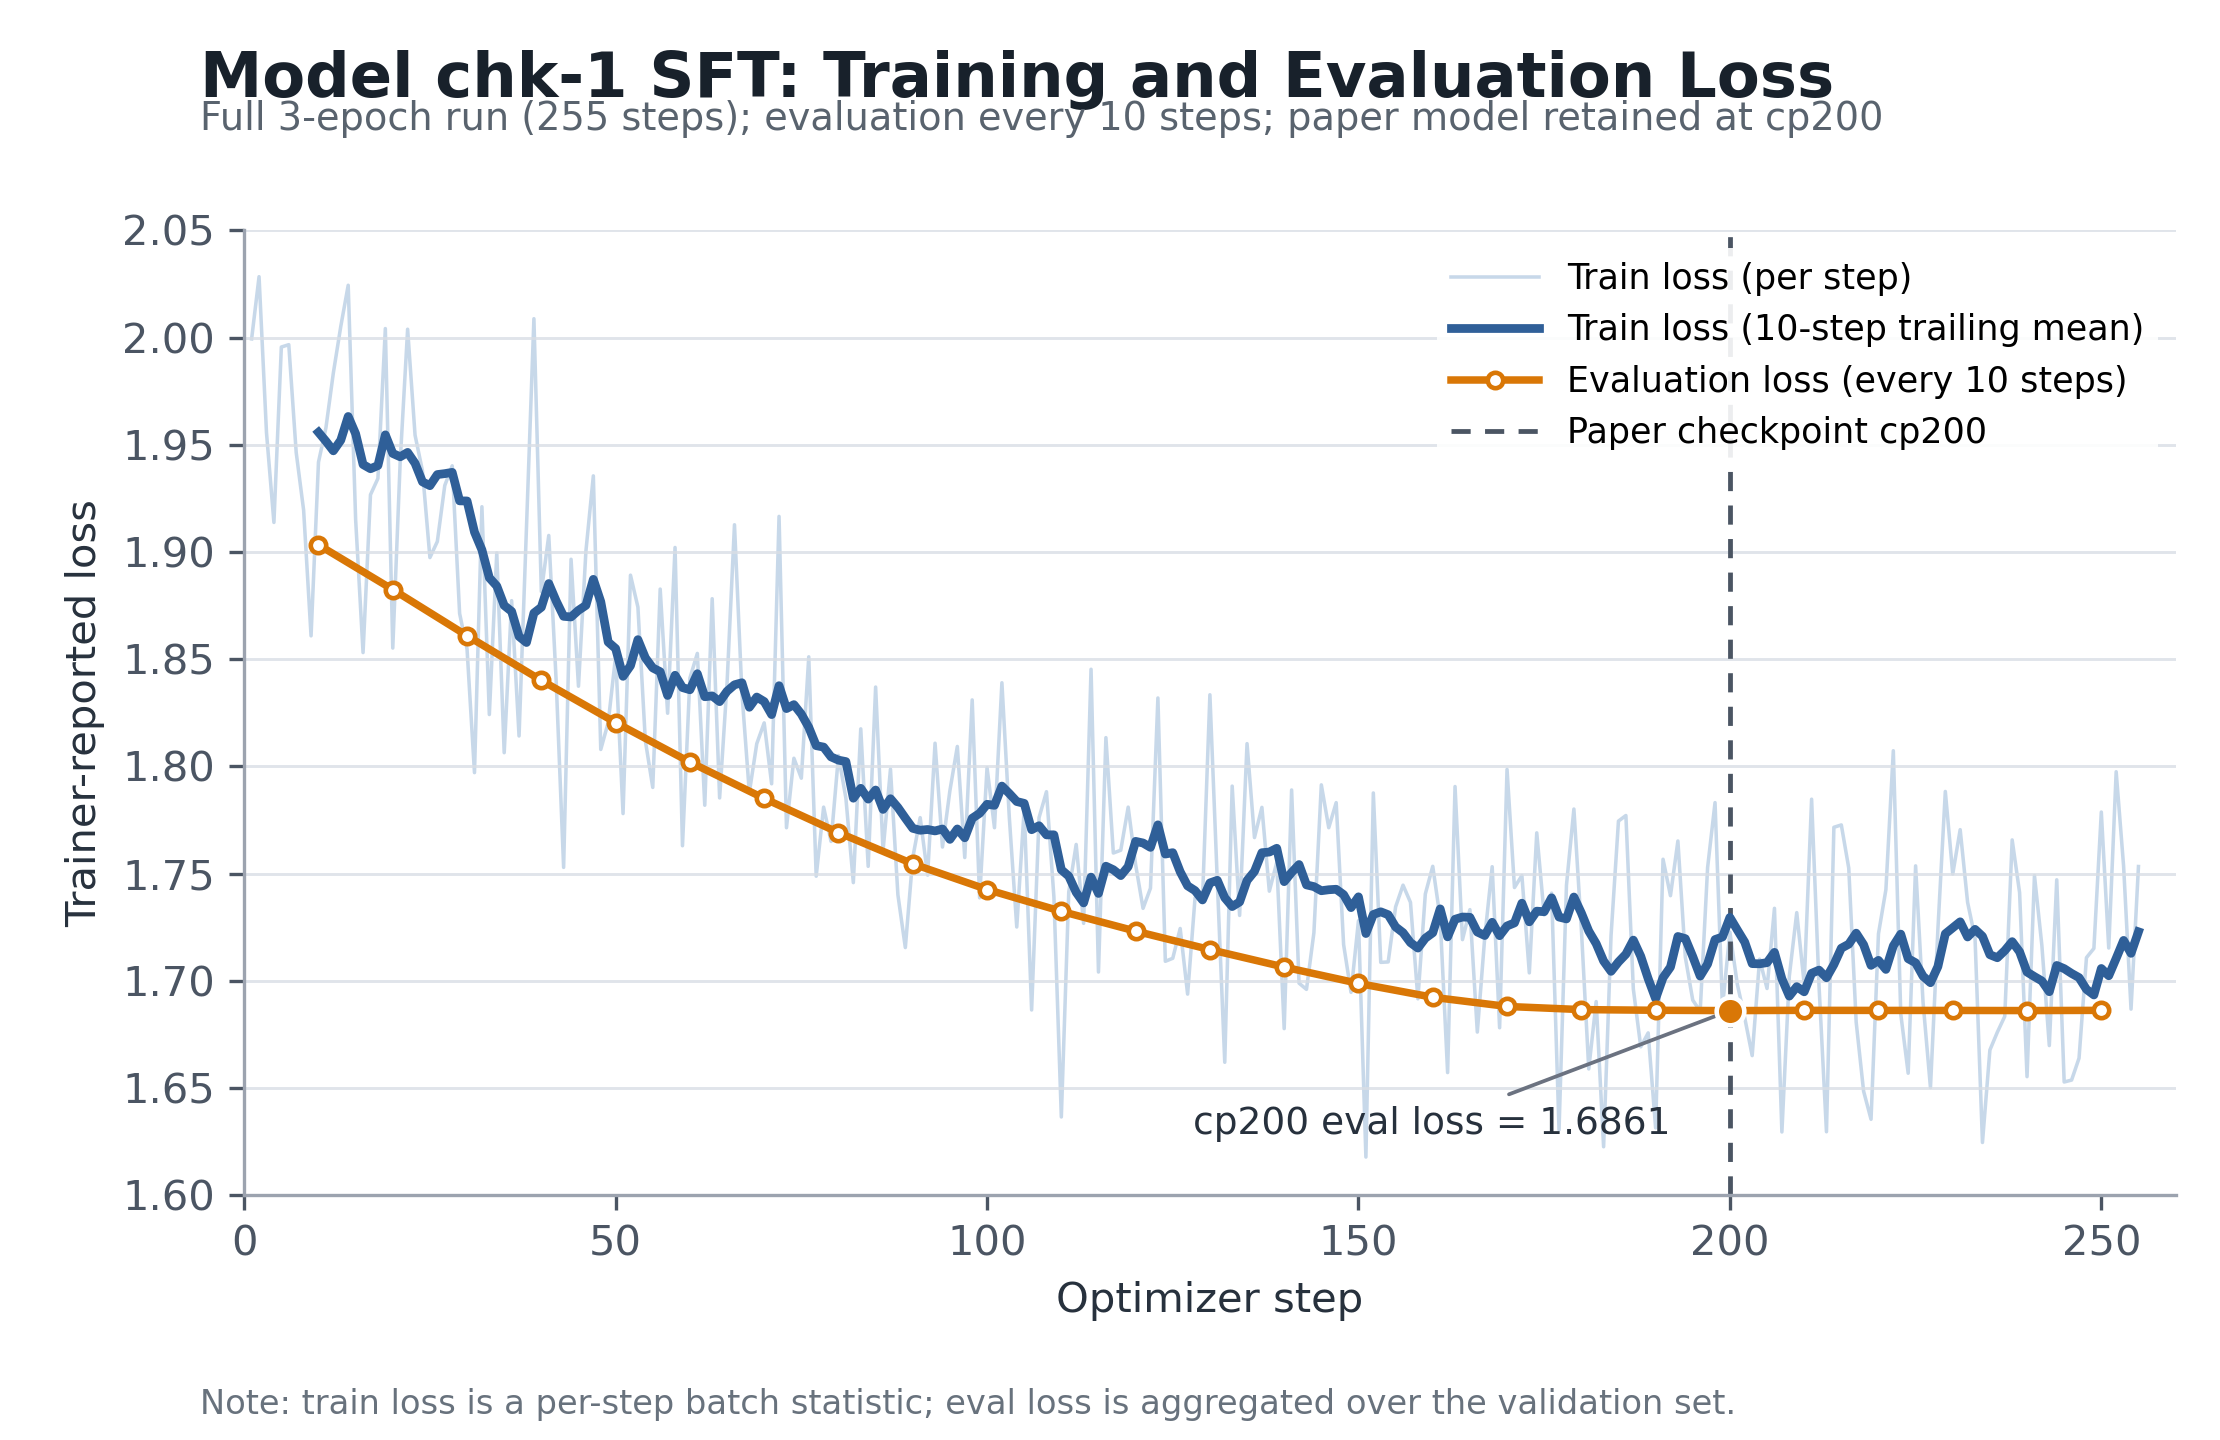
\includegraphics[width=0.9\textwidth]{Chapter2/Chapter2Figs/stage1_train/Model_chk-1_training_and_evaluation_loss.png}
            \caption{Training and evaluation loss for the archived analytical SFT run.}
            \label{fig:ch2:stage1_sft_loss}
    \end{center}
\end{figure}


In the frozen 255-step run, the 10-step trailing mean of training loss decreases from 1.9558 at step 10 to 1.7229 at step 255. Evaluation loss falls from 1.9033 at step 10 to its minimum logged value of 1.6861 at step 200, which is retained as the paper-facing \textit{Model chk-1} checkpoint, and subsequently remains nearly unchanged, reaching 1.6862 at the final scheduled evaluation at step 250. The continued modest decline in smoothed training loss after step 200, together with the plateau in evaluation loss, indicates diminishing generalization gains and a mild risk of overfitting, although no material increase in evaluation loss is observed.



Overall, \textbf{Checkpoint 200} is selected instead of the final checkpoint because it attains the lowest validation loss, 1.686099, with a token accuracy of 0.602685.  It also satisfies all generation-validity criteria in the eight-observation diagnostic sample: every completion terminates normally, conforms to the response format, remains below the token limit, and avoids periodic or catastrophic repetition. We also examined initial learning rates of \(5\times10^{-5}\), \(1\times10^{-5}\), and \(1\times10^{-6}\) through staged stability diagnostics under otherwise matched QLoRA settings. Detailed results are reported in Appendix~\ref{app:checkpoint_selection}.




\subsubsection*{Minutes-Style Paragraph-Rewriting SFT Results (\textit{Model chk-2})}



The Minutes-rewriting experiment implements the task-specific transition from
\textit{Model chk-1} to \textit{Model chk-2}. Specifically,
\textit{Model chk-2} is initialized from the exact-merged checkpoint 200 of
\textit{Model chk-1} and fine-tuned on the analysis-to-Minutes dataset described
in Section~\ref{ch2:sec:the-dataset}. Each target response concatenates the
rewriting teacher's fidelity reasoning trace, a literal \texttt{</think>}
boundary, and a single synthetic FOMC Minutes-style paragraph. Thus, the model
is trained to reproduce both the content-preservation reasoning process and the
resulting institutional rewrite, rather than to predict the corresponding
official Minutes directly. Training is performed for three epochs using
completion-only QLoRA, with a learning rate of $1.0\times10^{-6}$, a maximum
sequence length of 4,096 tokens, a per-device batch size of 1, and gradient
accumulation over 8 steps. With two training devices and 305 training samples,
the procedure completes after 60 optimization steps.



We also employed the hard gates in the checkpoint selection. For this training, each completion must satisfy the structure-and-delivery contract, preserve the source numeric multiset and date set, and remain free from capped or repetitive degeneration. Table~\ref{tab:app:chk2_checkpoint_selection_gates} summaried the hard gates for this training.


\begin{table}[htbp]
    \centering
    \footnotesize
    \setlength{\tabcolsep}{4pt}
    \renewcommand{\arraystretch}{1.14}

    \begin{tabularx}{\textwidth}{@{}
        >{\raggedright\arraybackslash}p{0.19\textwidth}
        >{\raggedright\arraybackslash}X
        >{\raggedright\arraybackslash}p{0.24\textwidth}
    @{}}
        \toprule
        \textbf{Screening criterion} &
        \textbf{Operational definition} &
        \textbf{Checkpoint-level requirement} \\
        \midrule

        Zero-tolerance structure and degeneration &
        Each completion must terminate with EOS, remain within the generation
        and 4,096-token sequence limits, contain exactly one
        \texttt{\textless/think\textgreater} boundary, and include nonempty
        reasoning followed by one 20--400-word paragraph. The final paragraph
        must contain no headings, lists, JSON, citations, credentials, or
        control markers. Strict periodic tails are prohibited, while full-text
        and tail four-gram repetition must remain below 0.50 and 0.60,
        respectively. &
        Zero such failures across all eight screening cases. \\

        Deterministic source fidelity &
        The normalized numeric multiset and the complete date and attribution
        sets must be preserved between the source analysis and the generated
        paragraph. Reuse of source phrases or sentences is permitted, but an
        exact copy of the complete source analysis is treated as a failure. &
        At least $75\%$ of the panel, corresponding to at least 6 of 8 cases,
        must pass. \\

        Validator A factual fidelity &
        For cases passing the complete deterministic check, a fresh Validator A
        call examines the source analysis, the student reasoning trace, and the
        rewritten paragraph. It verifies bidirectional claim support,
        reasoning--answer compatibility, and the preservation of quantities,
        dates, directions, comparisons, uncertainty, and attributions.
        Validator A does not receive the official Minutes reference. &
        At least $75\%$ of deterministic-pass cases must receive a strict
        Validator A PASS verdict. \\

        Validator B pass rate &
        Only cases passing Validator A are submitted to Validator B. Validator B
        receives the rewritten paragraph and the corresponding meeting's
        pre-action official Minutes, but not the source analysis or reasoning.
        It locates comparable official passages and evaluates the rewrite under
        the six-dimensional Minutes-style contract. &
        At least $50\%$ of Validator-A-pass cases must receive a strict
        Validator B PASS verdict. \\

        Validator B mean score &
        The six Validator B dimensions assess institutional register, sentence
        structure and information density, paragraph organization, attribution
        and hedging, temporal and comparative framing, and overall similarity
        to official Minutes prose. The checkpoint-level mean is calculated
        across all Validator-A-pass cases with valid scores, including cases
        that do not individually pass Validator B. &
        The checkpoint-level mean Validator B score must be at least 6.0 out
        of 10. \\

        Full-chain validity &
        A case is fully valid only when it passes the deterministic checks,
        Validator A, and Validator B in sequence:
        $H_{i,c}=D_{i,c}A_{i,c}B_{i,c}$. Per-case verdicts remain strict and are
        not altered by the relaxed checkpoint-level aggregation. &
        At least $25\%$ of the panel, corresponding to at least 2 of 8 cases,
        must satisfy the complete chain. \\

        Verification completeness &
        Every required validator call must reach a resolved terminal state.
        A contract-only remediation may resolve an incomplete validator report,
        but it must not change the generated candidate. &
        Zero unresolved validator, transport, or schema failures. \\

        Joint checkpoint decision &
        A checkpoint is eligible only if all checkpoint-level requirements
        above are satisfied simultaneously. If multiple checkpoints are
        eligible, they are ranked by full-chain pass rate, Validator B mean
        score, Validator A pass rate, deterministic-fidelity rate, and then the
        earlier checkpoint step. &
        Every checkpoint-level criterion must pass; no validation-loss or
        similarity result can compensate for a failed criterion. \\

        \bottomrule
    \end{tabularx}

    \caption{Relaxed checkpoint-selection screening criteria for
    \textit{Model chk-2}. The screening panel comprised eight deterministically
    selected validation cases and was used only for checkpoint selection.
    Checkpoint 50 was the only candidate satisfying every checkpoint-level
    requirement: 6 of 8 cases passed deterministic source fidelity, 5 of 6
    deterministic-pass cases passed Validator A, 3 of those 5 passed Validator
    B, the mean Validator B score was 6.73, and 3 of 8 cases passed the complete
    chain. Checkpoint 40 failed the Validator A, Validator B, and full-chain
    thresholds, whereas checkpoint 60 failed the Validator B pass-rate and
    full-chain thresholds. Checkpoint 50 was therefore retained.}
    \label{tab:app:chk2_checkpoint_selection_gates}
\end{table}


Across the 60-step SFT run, the per-step completion loss exhibited substantial
minibatch-level variation. Nevertheless, its seven-step trailing mean declined
from 1.6414 at step~10 to 1.5965 at step~60. The corresponding epoch-level
training-loss means were 1.6562, 1.5923, and 1.6014, indicating an initial
improvement followed by relative stabilization. Evaluation loss on the
42-sample monitoring split decreased monotonically at the ten-step evaluation
points, from 1.5647 at step~10 to its minimum logged value of 1.5262 at
step~60. The marginal improvement narrowed considerably toward the end of
training: evaluation loss declined from 1.5295 at step~40 to 1.5266 at
step~50 and then by only 0.000344, or 0.0225\%, between steps~50 and~60
(Figure~\ref{fig:ch2:stage2_sft}). The trajectory therefore approached an
in-run plateau without exhibiting material validation-loss deterioration.
Although checkpoint~60 attained the lowest monitoring loss, checkpoint
selection was not determined by loss alone. Checkpoint~50 was retained because
it was the only candidate among checkpoints~40, 50, and~60 to satisfy all of
the documented tolerant checkpoint-level quality criteria; checkpoint~40
failed the Validator~A, Validator~B, and full-chain thresholds, whereas
checkpoint~60 failed the Validator~B pass-rate and full-chain thresholds.

Accordingly, \textit{Checkpoint 50} is retained as the paper-facing
\textit{Model chk-2} adapter checkpoint for the subsequent diagnostic
evaluation. On the eight deterministically selected cases from the validation
split, checkpoint~50 produced no zero-tolerance structural or degeneration
failures; 6 of 8 cases passed the deterministic factual-fidelity screen, 5 of
those 6 passed Validator~A, and 3 of those 5 passed Validator~B, with a mean
Validator~B score of 6.73. Consequently, 3 of the 8 cases passed the complete
deterministic--Validator~A--Validator~B chain, exceeding the checkpoint-level
minimum of 25\%. Importantly, checkpoint~50 did not pass every sample-level
hard gate on all eight observations; it was selected because it was the only
candidate satisfying every tolerant aggregate admission criterion. The
complete candidate comparison and auxiliary semantic diagnostics are reported
in Appendix~\ref{app:checkpoint_selection}. Because this small validation panel was used for checkpoint selection, it provides selection evidence only and should not be interpreted as an external test or as population-level evidence
of rewriting performance.



\begin{figure}[htbp]
    \begin{center}
            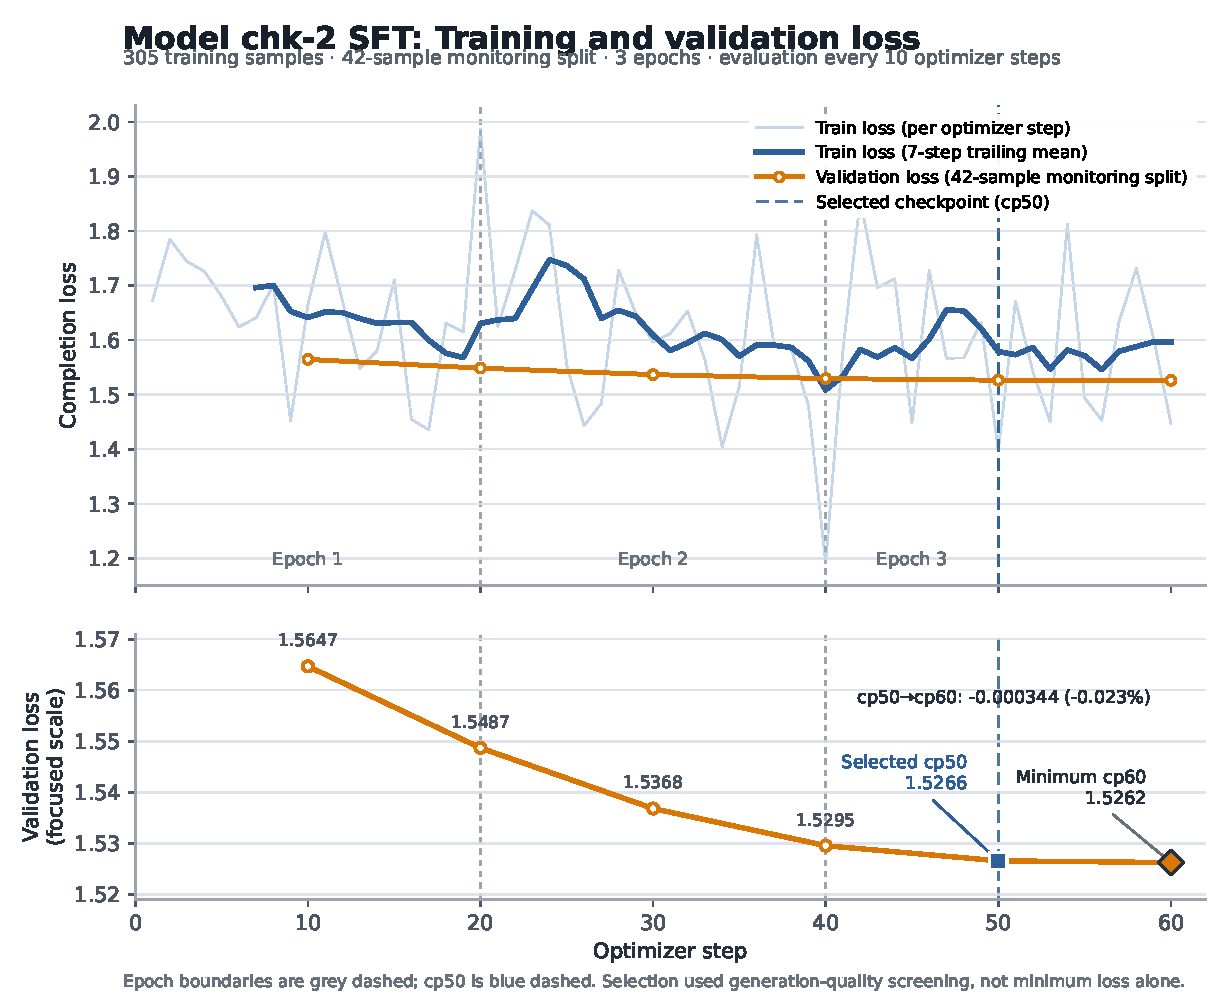
\includegraphics[width=0.9\textwidth]{Chapter2/Chapter2Figs/stage2_train/chk2_train_eval_loss_cp50.pdf}
            \caption{Training and evaluation loss for paragraph-rewriting SFT (\textit{Model chk-2}).}
            \label{fig:ch2:stage2_sft}
    \end{center}
\end{figure}




\subsubsection*{Policy-Decision GRPO Run (\textit{Model chk-3})}


For policy decision making prediction task, we further fine-tuned the \textit{Model chk-1} to get \textit{Model chk-3}. Here, we employed decision SFT for instruction following followed by decision GRPO for reasoning capacity improving. 

Decision SFT uses the fixed 312-row exposure schedule for 39 optimizer steps. Also, we added the following (Table~\ref{tab:app:chk3_sft_hard_gates}) to check the quality of the generation in checkpoint selection, including reasoning-boundary delivery, completion-cap control, the absence of periodic degeneration, and minimum direction and reward coverage for hold, hike, and cut.

\begin{table}[htbp]
\centering
\caption{Pre-GRPO SFT Qualification Gates for Model chk-3}
\label{tab:app:chk3_sft_hard_gates}
\footnotesize
\setlength{\tabcolsep}{5pt}
\renewcommand{\arraystretch}{1.15}
\begin{tabularx}{\textwidth}{
    @{}
    p{0.28\textwidth}
    p{0.27\textwidth}
    X
    @{}
}
\toprule
Hard gate & Frozen requirement & Purpose \\
\midrule

Reasoning-answer boundary
& Overall boundary rate $\geq .75$
& Ensures that the native reasoning section is properly separated from the terminal answer. \\

Completion cap
& Overall cap rate $\leq .25$
& Limits the frequency of outputs that reach the maximum completion length without valid termination. \\

Periodic degeneration
& Strict periodic-tail count $=0$
& Rejects checkpoints that generate mechanically repeated or periodic terminal sequences. \\

Direction coverage
& At least one sampled direction-correct output for each of hold, hike, and cut
& Verifies that all three policy directions remain reachable under stochastic decoding. \\

Nonzero-reward coverage
& At least one sampled nonzero-reward output for each of hold, hike, and cut
& Ensures that every direction provides a usable learning signal for GRPO initialization. \\

Reward dispersion
& Sampled reward standard deviation $>0$ for each direction
& Prevents zero-variance completion groups that provide no group-relative learning signal. \\
\bottomrule
\end{tabularx}
\end{table}

Finally, Figure~\ref{fig:ch2:chk3_sft_loss} illustrates the training and evaluation loss of the decision SFT stage. the five-step trailing mean of training loss decreases from 2.1035 at step 5 to 1.5592 at step 39, despite noticeable batch-level fluctuations. Evaluation loss declines consistently from 1.7539 at step 13 to 1.6222 at step 26 and reaches its minimum logged value of 1.6015 at step 39.


\begin{figure}[htbp]
    \centering
    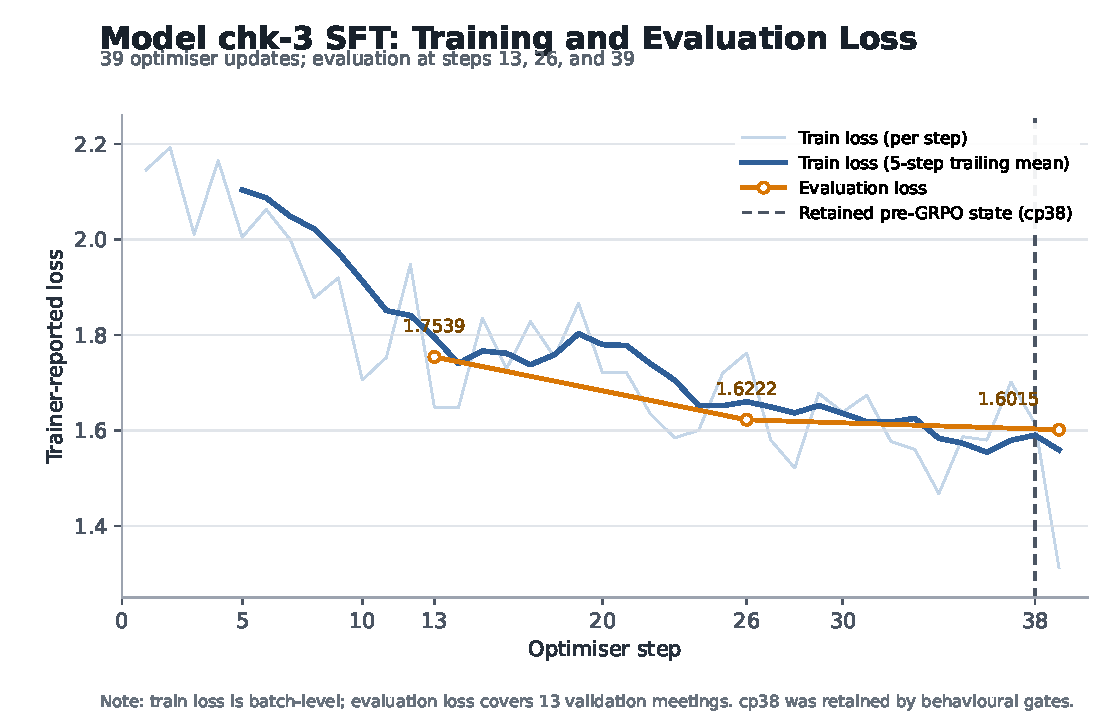
\includegraphics[width=0.90\textwidth]
    {Chapter2/Chapter2Figs/stage2_train/chk3_sft_train_eval_loss_cp38.pdf}
    \caption{Training and Evaluation Loss during the SFT Stage of Model chk-3}
    \label{fig:ch2:chk3_sft_loss}
\end{figure}


Exact-merged checkpoint 38 which has the similar loss as checkpoint 39 but passsed all 6 gates (checkpoint 39 failed Sampled cut-direction correctness test) is retained as the pre-GRPO state. 


Decision GRPO then starts from checkpoint 38, uses the same 312-row decision population for three epochs and four generations per prompt, and terminates at global step 468. Hard gates (Table~\ref{tab:app:chk3_grpo_hard_gates}) for this stage have been listed below:


\begin{table}[htbp]
\centering
\caption{GRPO Checkpoint-Selection Gates for Model chk-3}
\label{tab:app:chk3_grpo_hard_gates}
\footnotesize
\setlength{\tabcolsep}{5pt}
\renewcommand{\arraystretch}{1.15}
\begin{tabularx}{\textwidth}{
    @{}
    p{0.15\textwidth}
    p{0.24\textwidth}
    p{0.24\textwidth}
    X
    @{}
}
\toprule
Evaluation stage & Hard gate & Frozen requirement & Purpose \\
\midrule

Selection panel
& Delivery validity
& Delivery-valid rate $\geq .75$
& Restricts the shortlist to checkpoints that reliably satisfy the complete native-output contract. \\

Selection panel
& Completion cap
& Cap rate $\leq .25$
& Excludes checkpoints with excessive length-limit termination. \\

Selection panel
& Periodic degeneration
& Periodic-tail count $=0$
& Excludes checkpoints exhibiting strict periodic repetition. \\

\midrule

Blind panel
& Delivery validity
& Delivery-valid rate $\geq .75$
& Requires the delivery threshold to hold on an independent blind validation panel. \\

Blind panel
& Completion cap
& Cap rate $\leq .25$
& Requires completion-length stability to persist on the blind panel. \\

Blind panel
& Periodic degeneration
& Periodic-tail count $=0$
& Requires the absence of periodic degeneration on the blind panel. \\

\midrule

Retention panel
& Direction retention
& At least one direction-correct output for each of hold, hike, and cut
& Prevents checkpoint selection from eliminating any policy-action direction. \\

\bottomrule
\end{tabularx}
\end{table}

Finally, Figure~\ref{fig:ch2:chk3_grpo_reward} shows the evolution of the GRPO reward during training. The solid line reports the 20-step trailing mean, while the shaded region denotes \(\pm 1\) step-level standard error.


\begin{figure}[htbp]
    \centering
    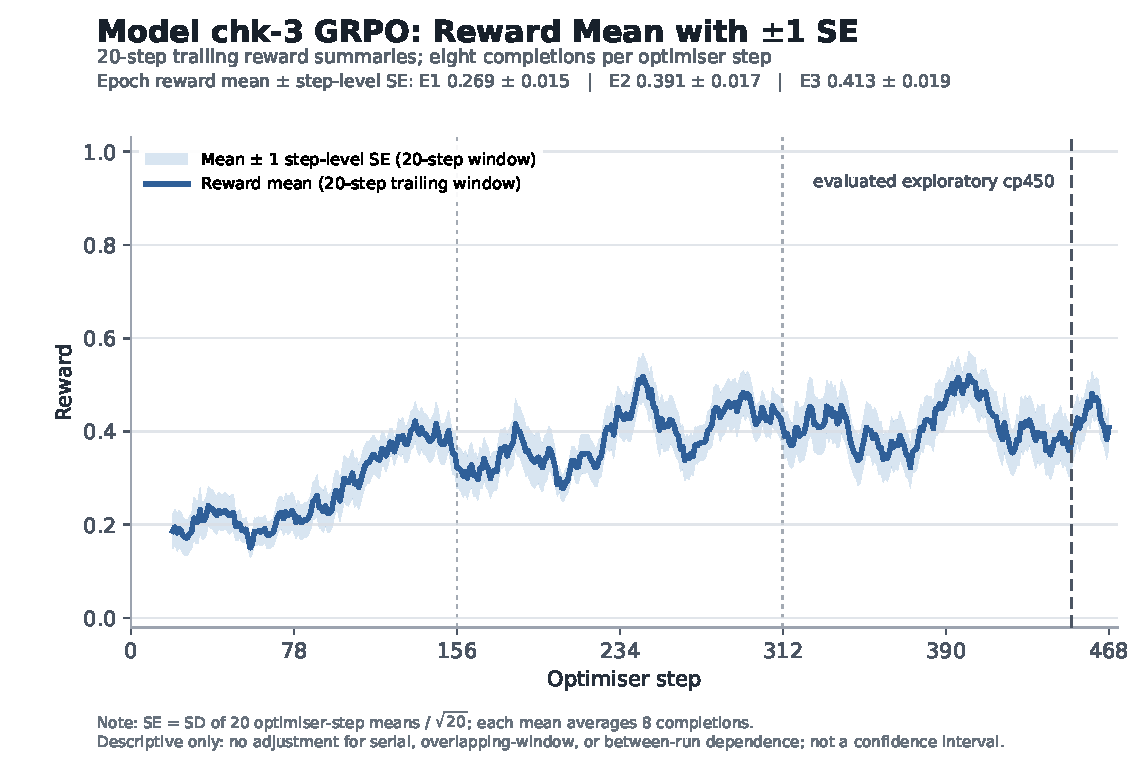
\includegraphics[width=\textwidth]{Chapter2/Chapter2Figs/stage2_train/chk3_grpo_reward_with_standard_error.pdf}
    \caption{GRPO Reward during Policy-Decision Training}
    \label{fig:ch2:chk3_grpo_reward}
\end{figure}


There is no checkpoint that has passed all 77 gates. Checkpoint 450 is selected as the \textit{Model chk-3} for post-GRPO evaluation because it is the best-observed exploratory candidate in the completed probe, not because it passed the preregistered selection gates. Its blind delivery-valid rate is 0.30, below the 0.75 gate. 



%%% end of decision making


\subsubsection*{Training Results Summary}

To summarize, the training evidence establishes \textit{Model chk-1} as the common parent of the independent Minutes-rewriting and policy-decision branches. \textit{Model chk-2} at checkpoint 50 is evaluated in the Minutes-rewriting diagnostics reported below. The two successive states of \textit{Model chk-3}, checkpoint 38 before GRPO and checkpoint 450 after GRPO, are evaluated separately on the policy-decision task. Table~\ref{tab:ch2:model_training_lineage} summarizes the models and their corresponding training methods.

\begin{table}[htbp]
    \centering
    \caption{Model Lineage and Training Summary}
    \label{tab:ch2:model_training_lineage}
    \footnotesize
    \setlength{\tabcolsep}{6pt}
    \renewcommand{\arraystretch}{1.15}
    \begin{tabularx}{\textwidth}{
        >{\raggedright\arraybackslash}p{0.20\textwidth}
        >{\raggedright\arraybackslash}p{0.24\textwidth}
        >{\raggedright\arraybackslash}p{0.20\textwidth}
        >{\raggedright\arraybackslash}X
    }
        \toprule
        Model name
        & Direct parent
        & Checkpoint
        & Training method \\
        \midrule

        \textit{Model chk-0}
        & DeepSeek-Distilled-llama3-8B
        & Pretrained release
        & Pretraining \\

        \textit{Model chk-1}
        & \textit{Model chk-0}
        & cp200
        & Analysis SFT \\

        \textit{Model chk-2}
        & \textit{Model chk-1} cp200
        & cp50
        & Minutes SFT \\

        \textit{Model chk-3}
        & \textit{Model chk-1} cp200
        & cp38, then cp450
        & Decision SFT, then Decision GRPO \\
        \bottomrule
    \end{tabularx}

    \begin{minipage}{0.97\textwidth}
        \scriptsize
        \textit{Note:} For Model chk-3, cp38 denotes the pre-GRPO
        Decision-SFT state, while cp450 denotes the evaluated post-GRPO
        state. These checkpoints are successive states of the same
        paper-level model, not separate models. Model chk-2 and Model chk-3 form independent downstream branches from Model chk-1.
    \end{minipage}
\end{table}



%%%%% end of model training result



\subsection*{Model Evaluation Results}

This subsection reports the evaluation results for the two downstream branches and their associated diagnostics. First, the Minutes-style paragraph-rewriting fidelity experiment primarily compares \textit{Model chk-2} with its immediate parent, \textit{Model chk-1}, while \textit{Model chk-0} serves as a background baseline. Second, as a target-relative prompt-sensitivity stress test, the LOO analysis measures how interventions to the Core 8 indicator blocks change the similarity of \textit{Model chk-2}'s output to a fixed synthetic reference; it does not establish information sufficiency. Third, the historical sentiment-Treasury diagnostic compares the estimated $\beta$ coefficients associated with texts generated by \textit{Model chk-0}, \textit{Model chk-1}, and \textit{Model chk-2}. Finally, the policy-decision evaluation compares \textit{Model chk-1} at checkpoint 200 with the pre-GRPO SFT state of \textit{Model chk-3} at checkpoint 38 and its post-GRPO state at checkpoint 450.



\subsubsection*{Minutes-Style Paragraph-Rewriting Fidelity and Similarity Performance}
This subsection reports the frozen checkpoint-50 reconstruction experiment on all 391 published Minutes-rewriting samples, covering 124 meetings from 28 January 2009 to 29 January 2025. It compares \textit{Model chk-0}, \textit{Model chk-1} checkpoint 200, and \textit{Model chk-2} checkpoint 50 using the same synthetic teacher references and \(K=10\) stochastic generations per sample and model, for \(391\times10\times3=11{,}730\) outputs. The 305 training, 42 validation, and 44 test rows retain their release labels, but all belong to a training-only release whose construction used official meeting text in sample selection. Only the 305 training rows supplied gradient updates; pooling the release therefore yields a reconstruction diagnostic, not an independent held-out evaluation. The separate 128-meeting historical Core8 panel covers 1993--2008 and supplies the subsequent prompt-sensitivity analysis, not this three-model similarity table.

% Canonical output: output/evaluation/retrain_v2/paper_chk2_text_similarity_all391_chk0_chk1_chk2cp50_vllm_t06_p09_k10_b1000_v1_20260901/
% Reproduction: Chapter2/review/minutes_primary_results_reconciliation_20260904.ipynb
% Derived paired tests: Chapter2/Chapter2Results/minutes_primary_meeting_paired_tests_20260904.csv

Table~\ref{tab:ch2:minutes_semantic_ttest} reports the paired differences in MPNet cosine similarity and BERTScore-F1 between successive model stages, comparing \textit{Model chk-1} with \textit{Model chk-0} and \textit{Model chk-2} with \textit{Model chk-1}.



\begin{table}[H]
    \centering
    \footnotesize
    \setlength{\tabcolsep}{3pt}
    \renewcommand{\arraystretch}{1.08}
    \caption{Paired Score Differences and Percentage Increases in
    Synthetic-Reference Semantic Similarity across Model Stages:
    124-Meeting Training-Release Reconstruction Diagnostic}
    \label{tab:ch2:minutes_semantic_ttest}

    \begin{threeparttable}
        \begin{tabularx}{\textwidth}{@{}
            >{\raggedright\arraybackslash}X
            *{3}{>{\centering\arraybackslash}p{0.235\textwidth}}
        @{}}
            \toprule
            & \multicolumn{3}{c}{\textbf{Model contrasts}} \\
            \cmidrule(lr){2-4}

            \textbf{Metric}
            & \makecell{
                \textit{chk1}\\
                \( - \)\\
                \textit{chk0}
            }
            & \makecell{
                \textit{chk2}\\
                \( - \)\\
                \textit{chk1}
            }
            & \makecell{
                \textit{chk2}\\
                \( - \)\\
                \textit{chk0}
            } \\
            \midrule

            \multicolumn{4}{@{}l}{
                \textit{Panel A: Paired differences in score levels}
            } \\
            \addlinespace[2pt]

            MPNet cosine
            & \(+0.005201^{***}\)
            & \(+0.002365^{**}\)
            & \(+0.007567^{***}\) \\[-1pt]

            & (5.886)
            & (2.845)
            & (8.057) \\

            \addlinespace

            BERTScore-F1
            & \(+0.003430^{***}\)
            & \(+0.000833^{**}\)
            & \(+0.004264^{***}\) \\[-1pt]

            & (12.440)
            & (2.936)
            & (12.916) \\

            \addlinespace[4pt]

            \multicolumn{4}{@{}l}{
                \textit{Panel B: Percentage increases relative to Model chk-0}
            } \\
            \addlinespace[2pt]

            MPNet cosine
            & \(+0.5552\%\)
            & \(+0.2525\%\)
            & \(+0.8077\%\) \\

            BERTScore-F1
            & \(+0.3584\%\)
            & \(+0.0871\%\)
            & \(+0.4455\%\) \\

            \bottomrule
        \end{tabularx}

        \begin{tablenotes}[flushleft]
            \scriptsize
            \item \textit{Notes:}
            In Panel A, the first row for each metric reports the paired mean
            difference, with a positive value indicating a higher
            raw-best-effort score for the later-stage model. Paired
            \(t\)-statistics are reported in parentheses. The 391 release rows
            are grouped into 124 meetings; scores are averaged across each
            meeting's rows and \(K=10\) stochastic generations before the
            paired tests are applied to the 124 equally weighted meeting-level
            observations (\(\mathrm{df}=123\)).
            \(^{*}p<0.05\), \(^{**}p<0.01\), and \(^{***}p<0.001\), based on
            supplementary, unadjusted two-sided paired \(t\)-tests computed
            from the frozen row scores. These are distinct from the
            hierarchical paired-bootstrap intervals discussed below.

            Raw best effort scores the recovered final text regardless of
            delivery-gate validity, assigning zero only to empty recovered
            text. It is not the four-gate reliability-adjusted measure used
            in the earlier checkpoint-318 historical experiment.

            Panel B reports, from left to right,
            \(100(\bar{S}_{1}-\bar{S}_{0})/\bar{S}_{0}\),
            \(100(\bar{S}_{2}-\bar{S}_{1})/\bar{S}_{0}\), and
            \(100(\bar{S}_{2}-\bar{S}_{0})/\bar{S}_{0}\), where
            \(\bar{S}_{j}\) is the equally weighted meeting-level mean score
            for model stage \(j\in\{0,1,2\}\). The Model chk-0 denominators are
            0.936793 for MPNet cosine and 0.957022 for BERTScore-F1. These
            percentage transformations are descriptive and are reported
            without \(t\)-statistics or significance markers.

            References are teacher-generated synthetic rewrites rather than
            official FOMC Minutes. Because all samples belong to the
            training-only release, these results are reconstruction
            diagnostics rather than leakage-safe estimates of held-out
            generalization.
        \end{tablenotes}
    \end{threeparttable}
\end{table}


Table~\ref{tab:ch2:minutes_semantic_ttest} reports positive paired mean differences across all three model contrasts. Relative to \textit{Model chk-0}, \textit{Model chk-1} increases MPNet cosine similarity by 0.005201 (\(t(123)=5.886\), \(p<0.001\)) and BERTScore-F1 by 0.003430 (\(t(123)=12.440\), \(p<0.001\)). These differences correspond to increases of 0.5552\% and 0.3584\%, respectively, relative to the corresponding \textit{Model chk-0} mean scores. The additional Minutes-rewriting stage produces smaller but statistically significant gains: relative to \textit{Model chk-1}, \textit{Model chk-2} increases MPNet cosine similarity by 0.002365 (\(t(123)=2.845\), \(p=0.0052\)) and BERTScore-F1 by 0.000833 (\(t(123)=2.936\), \(p=0.0040\)). When expressed relative to the \textit{Model chk-0} baselines, these incremental gains equal 0.2525\% and 0.0871\%, respectively. Across the complete training lineage, \textit{Model chk-2} exceeds \textit{Model chk-0} by 0.007567 in MPNet cosine similarity (\(t(123)=8.057\), \(p<0.001\)) and by 0.004264 in BERTScore-F1 (\(t(123)=12.916\), \(p<0.001\)), equivalent to relative increases of 0.8077\% and 0.4455\%. Although the paired tests reject equality of the meeting-level means, the absolute and percentage improvements remain modest. Moreover, the comparison measures reconstruction similarity to synthetic teacher-generated references drawn from the training-only release; it does not establish held-out generalization, factual superiority, or equivalence with official FOMC Minutes.

The inferential procedure matters for the smaller incremental gains. The
frozen experiment's 1,000-draw hierarchical paired bootstrap, which resamples
meetings within release splits and stochastic replicates, gives 95\%
intervals of \([-0.000556,\ 0.005239]\) for the \textit{chk-2} minus
\textit{chk-1} MPNet difference and \([-0.000090,\ 0.001823]\) for
BERTScore-F1. Both intervals include zero. The frozen meeting-level
sign-flip tests give six-comparison Holm-adjusted \(p\)-values of 0.00524
and 0.00494, respectively; these tests also operate on averaged meeting
differences and are distinct from the hierarchical bootstrap. Thus, the supplementary paired
\(t\)-tests on the averaged meeting scores reject equality at the 1\%
level, while the hierarchical intervals retain uncertainty about the sign
of these incremental gains. The results support modest reconstruction
improvements under the reported scoring rule, with inference qualified by
the treatment of stochastic-generation variability.


%%%% end of Minutes-generation fidelity and similarity results

\subsubsection*{Core 8 Indicators Leave-One-Out Sensitivity Results}

This subsection estimates the target-relative sensitivity of \textit{Model chk-2} to the eight Core8 economic-topic blocks. The historical panel contains 128 regular FOMC meetings from 1993--2008 and 10 fixed stochastic generation seeds.  For each meeting, the evaluation includes one Full prompt, eight exact-deletion variants, and eight token-count-matched neutral-replacement variants, yielding \(128 \times 17 \times 10 = 21{,}760\) fresh outputs.  


Table~\ref{tab:ch2:core8_loo_ttest} reports the paired leave-one-out differences in MPNet cosine similarity and BERTScore-F1 for each topic under the two intervention designs. The Full and intervened outputs are evaluated against the same deterministic synthetic reference, and uncertainty is estimated using 10,000 shared-index hierarchical paired-bootstrap draws at the meeting level. A positive estimates indicate weaker semantic retention following the corresponding intervention.


\begin{table}[H]
    \centering
    \scriptsize
    \setlength{\tabcolsep}{3pt}
    \renewcommand{\arraystretch}{1.00}
    \caption{Core8 Indicators Leave-One-Out Sensitivity Results for
    \textit{Model chk-2} (Checkpoint 50).}
    \label{tab:ch2:core8_loo_ttest}
    \begin{threeparttable}
        \begin{tabularx}{\textwidth}{
            @{}
            >{\raggedright\arraybackslash}p{0.21\textwidth}
            >{\centering\arraybackslash}X
            >{\centering\arraybackslash}X
            >{\centering\arraybackslash}X
            >{\centering\arraybackslash}X
            @{}
        }
            \toprule
            & \multicolumn{2}{c}{
                \textbf{Full \( - \) Exact deletion}
            }
            & \multicolumn{2}{c}{
                \textbf{Full \( - \) Neutral replacement}
            } \\
            \cmidrule(lr){2-3}
            \cmidrule(lr){4-5}

            \textbf{Indicator}
            & \makecell{\textbf{MPNet}\\\textbf{cosine}}
            & \makecell{\textbf{BERTScore}\\\textbf{F1}}
            & \makecell{\textbf{MPNet}\\\textbf{cosine}}
            & \makecell{\textbf{BERTScore}\\\textbf{F1}} \\
            \midrule

            Consumer Price Index (CPI)
            & \makecell{\(+0.016115^{***}\)\\\((4.796)\)}
            & \makecell{\(+0.011090^{***}\)\\\((4.297)\)}
            & \makecell{\(+0.045634^{***}\)\\\((13.637)\)}
            & \makecell{\(+0.027250^{***}\)\\\((11.184)\)} \\

            \addlinespace

            GDP Growth
            & \makecell{\(-0.010557\)\\\((-2.586)\)}
            & \makecell{\(+0.006047\)\\\((2.063)\)}
            & \makecell{\(-0.019066^{***}\)\\\((-5.598)\)}
            & \makecell{\(+0.001441\)\\\((0.578)\)} \\

            \addlinespace

            Government Purchases
            & \makecell{\(+0.003228\)\\\((0.926)\)}
            & \makecell{\(+0.014988^{***}\)\\\((6.033)\)}
            & \makecell{\(-0.000921\)\\\((-0.280)\)}
            & \makecell{\(+0.011643^{***}\)\\\((5.008)\)} \\

            \addlinespace

            Housing Starts
            & \makecell{\(+0.006132\)\\\((1.550)\)}
            & \makecell{\(+0.003320\)\\\((1.235)\)}
            & \makecell{\(+0.007800\)\\\((2.365)\)}
            & \makecell{\(+0.007697^{**}\)\\\((3.643)\)} \\

            \addlinespace

            Industrial Production
            & \makecell{\(-0.001850\)\\\((-0.567)\)}
            & \makecell{\(+0.007704^{*}\)\\\((3.161)\)}
            & \makecell{\(-0.000096\)\\\((-0.028)\)}
            & \makecell{\(+0.008217^{*}\)\\\((3.334)\)} \\

            \addlinespace

            Labour Market
            & \makecell{\(-0.010267\)\\\((-2.990)\)}
            & \makecell{\(+0.008031^{*}\)\\\((3.268)\)}
            & \makecell{\(-0.012535^{**}\)\\\((-3.663)\)}
            & \makecell{\(+0.005386\)\\\((2.301)\)} \\

            \addlinespace

            Money Supply
            & \makecell{\(-0.011866^{*}\)\\\((-3.436)\)}
            & \makecell{\(+0.004356\)\\\((1.764)\)}
            & \makecell{\(-0.014813^{**}\)\\\((-4.118)\)}
            & \makecell{\(-0.001646\)\\\((-0.616)\)} \\

            \addlinespace

            Unemployment Rate
            & \makecell{\(-0.013541^{**}\)\\\((-3.849)\)}
            & \makecell{\(-0.004076\)\\\((-1.608)\)}
            & \makecell{\(-0.015119^{***}\)\\\((-4.535)\)}
            & \makecell{\(-0.004263\)\\\((-1.717)\)} \\

            \bottomrule
        \end{tabularx}

        \begin{tablenotes}[flushleft]
            \tiny

            \item \textit{Notes:}
            Each point estimate is the raw semantic-similarity score for the
            full Core8 prompt minus the corresponding score after intervention.
            A positive value therefore indicates that deleting or neutralizing
            the indicator reduces similarity to the fixed, source-grounded
            synthetic Minutes reference; the reference is not official FOMC
            Minutes.

            \item Values in parentheses are paired \(t\)-statistics calculated
            from 128 meeting-level differences after first averaging the
            \(K=10\) paired stochastic replicates within each meeting. Meetings
            receive equal weight, and all tests have 127 degrees of freedom.

            \item The 32 two-sided \(p\)-values are adjusted jointly using the
            Holm procedure.
            \(^{*}p_{\mathrm{Holm}}<0.05\),
            \(^{**}p_{\mathrm{Holm}}<0.01\), and
            \(^{***}p_{\mathrm{Holm}}<0.001\).

            \item These paired \(t\)-tests are supplemental parametric
            summaries calculated from the frozen \(K=10\) meeting-level
            differences. The primary uncertainty analysis is the 10,000-draw
            shared-index hierarchical paired bootstrap. Its
            percentile intervals are not adjusted for multiplicity.

            \item Holm-adjusted \(t\)-test classifications need not coincide
            with the unadjusted bootstrap intervals. The GDP Growth and Labour
            Market exact-deletion MPNet intervals exclude zero, but their
            Holm-adjusted \(t\)-test \(p\)-values are \(0.1626\) and \(0.0536\),
            respectively, and therefore receive no significance marker.

            \item All 21,760 requested outputs remain in the semantic estimand,
            five empty extracted answers are scored as zero. The structure,
            numeric/date-fidelity, and repetition gates are diagnostic only:
            208 outputs pass the joint gate, and gate failures neither remove
            rows nor zero-penalize nonempty outputs.
        \end{tablenotes}
    \end{threeparttable}
\end{table}




Table~\ref{tab:ch2:core8_loo_ttest} reveals substantial heterogeneity in the
target-relative sensitivity of \textit{Model chk-2} across the eight Core8
topic blocks. Of the 32 intervention--metric comparisons, 16 remain
statistically significant after joint Holm adjustment: seven under exact
deletion and nine under token-matched neutral replacement. These comprise
eight MPNet-cosine and eight BERTScore-F1 comparisons, with ten significant
positive estimates and six significant negative estimates. The primary
hierarchical-bootstrap intervals exclude zero for 18 cells; however, these
intervals are not adjusted for multiplicity. The two additional
interval-excluding cells are the exact-deletion MPNet contrasts for GDP Growth
and the Labour Market, whose Holm-adjusted \(p\)-values are 0.1626 and 0.0536,
respectively.


CPI is the only indicator with Holm-significant effects in all four
intervention--metric cells. Exact deletion produces differences of
\(+0.016115\) for MPNet cosine and \(+0.011090\) for BERTScore-F1, whereas
neutral replacement produces larger differences of \(+0.045634\) and
\(+0.027250\), respectively. All four contrasts satisfy
\(p_{\mathrm{Holm}}<0.001\). The neutral-replacement MPNet estimate is also the
largest absolute effect reported in the table. Thus, CPI exhibits the most
consistently positive association with target-relative similarity across both
intervention designs and semantic metrics. The larger neutral-replacement
estimates indicate that preserving prompt length does not preserve alignment
with the fixed synthetic reference when CPI-specific information is replaced.
Nevertheless, the difference between deletion and neutral replacement should
not be interpreted causally because the two interventions alter the prompt in
different ways.


The remaining results are more dependent on the intervention and metric.
Government Purchases has significant positive BERTScore-F1 differences under
both exact deletion (\(\Delta=0.014988\)) and neutral replacement
(\(\Delta=0.011643\)), while neither MPNet contrast is significant. Industrial
Production follows a similar BERTScore-specific pattern, with significant
positive differences of 0.007704 and 0.008217 under the two interventions.
Housing Starts is significant only for BERTScore-F1 under neutral replacement
(\(\Delta=0.007697\), \(p_{\mathrm{Holm}}<0.01\)). The Labour Market exhibits
a mixed pattern: exact deletion produces a significant positive
BERTScore-F1 difference (\(\Delta=0.008031\)), whereas neutral replacement
produces a significant negative MPNet difference
(\(\Delta=-0.012535\)).


Several topics exhibit significant negative MPNet estimates. GDP Growth is
significant only under neutral replacement
(\(\Delta=-0.019066\), \(p_{\mathrm{Holm}}<0.001\)). Money Supply has
significant negative MPNet differences under both exact deletion
(\(\Delta=-0.011866\)) and neutral replacement
(\(\Delta=-0.014813\)), as does the Unemployment Rate
(\(\Delta=-0.013541\) and \(\Delta=-0.015119\), respectively). Because the
contrast is defined as the Full-prompt score minus the intervention score,
these negative estimates indicate that the intervened outputs are, on average,
more similar to the fixed synthetic reference. They do not demonstrate that
removing the corresponding information improves factual accuracy or economic
quality.


Overall, CPI is the only topic with consistently positive and
Holm-significant sensitivity across both interventions and both metrics.
Government Purchases and Industrial Production exhibit positive sensitivity
primarily through BERTScore-F1, while the results for Housing Starts and the
Labour Market are intervention-specific. GDP Growth, Money Supply, and the
Unemployment Rate instead display significant negative MPNet effects in at
least one intervention. These findings measure how Core8 prompt interventions
change the similarity of \textit{Model chk-2}'s output to a fixed,
teacher-generated synthetic reference; they do not identify causal topic
importance, information sufficiency, factual correctness, or similarity to
official FOMC Minutes. Moreover, because all 32 cells trigger at least one
prespecified replicate-adequacy condition, borderline estimates should be
interpreted cautiously and may require additional paired generations.

%%%% end of Core8 LOO sensitivity results



\subsubsection*{Historical Sentiment--Federal Funds Futures Association Results}

TThis subsection examines whether coefficients recovered from model-generated documents resemble those recovered from official FOMC Minutes given a empirical model. We employed the test from \citet{tadle2022fomc} which examines whether the change of Federal Funds futures is affected by the FOMC minutes' sentiments. 


We use the same dataset as the original test, including daily 30-Day Federal Funds futures returns from December 1, 2004, through April 30, 2015. It includes 83 FOMC meetings, of which 82 provide estimable news-shock events. Depending on contract horizon, the regressions contain between 2,338 and 2,613 daily observations. Besides the official Minutes, we included the synthetic documents generated from \textit{Model chk-0}, \textit{Model chk-1} , and \textit{Model chk-2}.

Document sentiment is measured using the Loughran-McDonald dictionary polarity score. For each generated source, the meeting-level score is constructed from 10 stochastic document replicates. 


Table~\ref{tab:ch2:tadle_post_beta} reports the post-2011 marginal coefficient ($\widehat{\beta}^{\,\mathrm{post}} = \widehat{\beta}_{NS} + \widehat{\beta}_{\mathrm{post}\times NS}$) for each document source and futures horizon.


Then, Table~\ref{tab:ch2:tadle_beta_distance} reports the direct
bootstrap estimates of the coefficient distances in
Eq.~\ref{eq:ch2:tadle_beta_distance} and the \textit{Model chk-2} gains in
Eq.~\ref{eq:ch2:tadle_beta_gain}.


A smaller absolute coefficient distance indicates closer agreement with the coefficient estimated from the official Minutes. Uncertainty is quantified using 10,000 paired, regime-stratified calendar-year block-bootstrap draws, with 2011 retained in every draw and the 10 generated-document replicates resampled within meetings using indices shared across model arms.



\begin{table}[htbp]
    \centering
    \footnotesize
    \setlength{\tabcolsep}{6pt}
    \renewcommand{\arraystretch}{1.12}
    \caption{Post-2011 Marginal Federal Funds Futures Price-Return Coefficients}
    \label{tab:ch2:tadle_post_beta}

    \begin{threeparttable}
    \begin{tabularx}{\textwidth}{
        @{}
        l
        >{\centering\arraybackslash}p{0.09\textwidth}
        *{4}{>{\centering\arraybackslash}X}
        @{}
    }
        \toprule
        \textbf{Horizon}
        & \(\boldsymbol{N}\)
        & \makecell{\textbf{Official}\\\textbf{Minutes}}
        & \textit{Model chk-0}
        & \makecell{\textit{Model chk-1}\\cp200}
        & \makecell{\textit{Model chk-2}\\cp50} \\
        \midrule

        FF1
        & 2,613
        & \makecell{\(-0.0833\)\\\((0.1034)\)}
        & \makecell{\(-0.0421\)\\\((0.1014)\)}
        & \makecell{\(-0.0765\)\\\((0.0788)\)}
        & \makecell{\(-0.0535\)\\\((0.0889)\)} \\

        \addlinespace

        FF3
        & 2,612
        & \makecell{\(-0.3490\)\\\((0.1584)\)}
        & \makecell{\(+0.0139\)\\\((0.1411)\)}
        & \makecell{\(+0.0075\)\\\((0.1199)\)}
        & \makecell{\(+0.0062\)\\\((0.1279)\)} \\

        \addlinespace

        FF6
        & 2,612
        & \makecell{\(-0.7240\)\\\((0.2867)\)}
        & \makecell{\(-0.0718\)\\\((0.2500)\)}
        & \makecell{\(+0.0183\)\\\((0.2273)\)}
        & \makecell{\(-0.0355\)\\\((0.2147)\)} \\

        \addlinespace

        FF12
        & 2,338
        & \makecell{\(-1.5981\)\\\((0.6395)\)}
        & \makecell{\(+0.0867\)\\\((0.4961)\)}
        & \makecell{\(+0.2032\)\\\((0.4014)\)}
        & \makecell{\(+0.0242\)\\\((0.4248)\)} \\

        \bottomrule
    \end{tabularx}

    \begin{tablenotes}[flushleft]
        \scriptsize
        \item \textit{Notes:}
        Each cell reports the post-August 8, 2011 marginal coefficient
        \(
        \widehat{\beta}^{\,\mathrm{post}}
        =
        \widehat{\beta}_{NS}
        +
        \widehat{\beta}_{\mathrm{post}\times NS}
        \)
        in basis points of the Federal Funds futures price log return per
        one-unit constructed news shock. A unit is defined by the news-shock
        regressor formed from Minutes and Statement components standardized
        separately by source; the news shock is not itself re-standardized to
        unit variance. The quantity is not a policy-rate change. HC1
        heteroskedasticity-robust standard errors are in parentheses. The
        regressions control for the contemporaneous VIX log change, the
        post-2011 indicator, and calendar-year fixed effects.
    \end{tablenotes}
    \end{threeparttable}
\end{table}


\begin{table}[htbp]
    \centering
    \scriptsize
    \setlength{\tabcolsep}{3pt}
    \renewcommand{\arraystretch}{1.14}
    \caption{Post-2011 Coefficient Distances and Direct Model chk-2 Distance Gains}
    \label{tab:ch2:tadle_beta_distance}

    \begin{threeparttable}
    \begin{tabularx}{\textwidth}{
        @{}
        l
        *{5}{>{\centering\arraybackslash}X}
        @{}
    }
        \toprule
        \textbf{Horizon}
        & \makecell{\(\boldsymbol{D_{0,O}}\)\\chk-0}
        & \makecell{\(\boldsymbol{D_{1,O}}\)\\chk-1}
        & \makecell{\(\boldsymbol{D_{2,O}}\)\\chk-2}
        & \makecell{\(\boldsymbol{G_0}\)\\chk-2 vs. chk-0}
        & \makecell{\(\boldsymbol{G_1}\)\\chk-2 vs. chk-1} \\
        \midrule

        FF1
        & \makecell{\(0.0412\)\\\([0.0026,\,0.2446]\)}
        & \makecell{\(0.0068\)\\\([0.0014,\,0.1858]\)}
        & \makecell{\(0.0298\)\\\([0.0023,\,0.2376]\)}
        & \makecell{\(+0.0114\)\\\([-0.1290,\,+0.1449]\)}
        & \makecell{\(-0.0229\)\\\([-0.1717,\,+0.1167]\)} \\

        \addlinespace

        FF3
        & \makecell{\(0.3629\)\\\([0.1817,\,0.6122]\)}
        & \makecell{\(0.3565\)\\\([0.1643,\,0.6367]\)}
        & \makecell{\(0.3552\)\\\([0.1921,\,0.6176]\)}
        & \makecell{\(+0.0077\)\\\([-0.2449,\,+0.2469]\)}
        & \makecell{\(+0.0013\)\\\([-0.2811,\,+0.2866]\)} \\

        \addlinespace

        FF6
        & \makecell{\(0.6523\)\\\([0.2723,\,1.3163]\)}
        & \makecell{\(0.7423\)\\\([0.2939,\,1.5051]\)}
        & \makecell{\(0.6885\)\\\([0.3152,\,1.5384]\)}
        & \makecell{\(-0.0363\)\\\([-0.6369,\,+0.4806]\)}
        & \makecell{\(+0.0538\)\\\([-0.6017,\,+0.7263]\)} \\

        \addlinespace

        FF12
        & \makecell{\(1.6848\)\\\([0.3899,\,4.2564]\)}
        & \makecell{\(1.8013\)\\\([0.5735,\,4.3401]\)}
        & \makecell{\(1.6223\)\\\([0.5374,\,3.9242]\)}
        & \makecell{\(+0.0625\)\\\([-1.2649,\,+1.5157]\)}
        & \makecell{\(+0.1790\)\\\([-1.4377,\,+1.8551]\)} \\

        \bottomrule
    \end{tabularx}

    \begin{tablenotes}[flushleft]
        \scriptsize
        \item \textit{Notes:}
        \(D_{m,O}=|\widehat{\beta}_{m,\mathrm{post}}-
        \widehat{\beta}_{O,\mathrm{post}}|\). The direct gain is
        \(G_j=D_{j,O}-D_{2,O}\), so a positive value indicates that
        \textit{Model chk-2} is closer to the official-Minutes coefficient
        than comparator \(j\). Brackets are 95\% paired percentile-bootstrap
        intervals computed directly, draw by draw, for each distance or gain.
        A distance interval is descriptive uncertainty, not an equivalence or
        model-minus-official null test. Gain inference uses a prespecified
        eight-test Holm family; no gain is significant after adjustment.
    \end{tablenotes}
    \end{threeparttable}
\end{table}


% The official-Minutes post-2011 coefficients become increasingly negative as the
% contract horizon lengthens, whereas the generated-source coefficients remain
% closer to zero. Across the four horizons, the unweighted mean absolute distance
% from the official coefficient is \(0.6853\) basis points for \textit{Model
% chk-0}, \(0.7267\) for \textit{Model chk-1}, and \(0.6739\) for \textit{Model
% chk-2}. Thus, \textit{Model chk-2} has the smallest descriptive mean distance,
% but the horizon-specific ordering is not uniform: \textit{Model chk-1} is
% closest at FF1, \textit{Model chk-2} at FF3 and FF12, and \textit{Model chk-0}
% at FF6.




Overall, the coefficient-distance results provide only qualified descriptive
evidence that \textit{Model chk-2} is, on average, slightly closer to the
coefficient estimated from the official Minutes. Across the four futures
horizons, its unweighted mean absolute distance is \(0.6739\) basis points,
compared with \(0.6853\) for \textit{Model chk-0} and \(0.7267\) for
\textit{Model chk-1}. The horizon-specific ordering is not uniform:
\textit{Model chk-1} is closest at FF1, \textit{Model chk-2} is closest at FF3
and FF12, and \textit{Model chk-0} is closest at FF6. At FF12,
\textit{Model chk-2} records a distance of \(D_{2,O}=1.6223\), compared with
\(1.6848\) for \textit{Model chk-0} and \(1.8013\) for
\textit{Model chk-1}. The advantage at this horizon is therefore smaller than
suggested by the previous estimates but remains the largest descriptive
distance gain for \textit{Model chk-2}. Importantly, all eight prespecified
direct paired distance-gain tests were conducted. Every 95\% bootstrap
confidence interval crosses zero, and none of the gains remains significant
after Holm adjustment. The results therefore support only the narrower
conclusion that \textit{Model chk-2} achieves the smallest descriptive
four-horizon mean distance and is closest to the official-Minutes coefficient
at two horizons.




% decision making accuracy 

\subsubsection*{Decision Prediction Performance}

This subsection assesses how effectively the separate policy-decision branch uses target-neutral pre-meeting information to predict realized federal funds rate decisions. It compares the predictive performance of supervised fine-tuning and subsequent GRPO across the pooled evaluation panel and benchmarks the LLM checkpoints against persistence-based, econometric, machine-learning, and market-implied baselines on a matched historical panel.


The first analysis evaluates the policy-direction performance of four LLM checkpoints across the pooled panel of 31 meetings. The second assesses exact-action accuracy, which requires both the predicted direction and the predicted basis-point magnitude to match the realized policy decision. The third benchmarks the LLM checkpoints against five operational baselines using the mean probability assigned to the realized policy direction in the 19-meeting historical external panel (H19).


%%%%% llm accuarcy
\paragraph*{Policy-direction Performance.} The first subsection examines decision-prediction performance across the combined historical external and post-cutoff evaluation panels. The pooled analysis includes 31 regular FOMC meetings, 19 from the historical external panel and 12 from the post-cutoff panel, with 10 stochastic generations per model. We evaluate \textit{Model chk-0}, \textit{Model chk-1} at checkpoint 200, and the two successive states of \textit{Model chk-3}: SFT checkpoint 38 and GRPO checkpoint 450. This produces \(31 \times 10 \times 4 = 1{,}240\) model predictions.


Table~\ref{tab:ch2:decision_pooled_n31} reports direction accuracy, three-class (Cut, Hold, Hike) balanced accuracy, class-specific recall, and meeting-level modal accuracy. Table~\ref{tab:ch2:decision_pooled_action_magnitude} further reports exact-action accuracy by realized policy direction and basis-point magnitude. Because the two panels were pooled after their separate frozen evaluations, these results constitute a post-hoc descriptive comparison rather than a new prospective or out-of-sample validation exercise. In particular, all five hike meetings come from the historical external panel, whereas the post-cutoff panel contains only cut and hold decisions.


\begin{table}[H]
    \centering
    \footnotesize
    \setlength{\tabcolsep}{3.5pt}
    \renewcommand{\arraystretch}{1.15}
    \begin{threeparttable}
    \caption{Post-Hoc Pooled Decision Prediction Performance
    (\(N=31\), \(K=10\))}
    \label{tab:ch2:decision_pooled_n31}
    
    \begin{tabularx}{\textwidth}{@{}
        >{\raggedright\arraybackslash}X
        >{\centering\arraybackslash}p{0.17\textwidth}
        >{\centering\arraybackslash}p{0.17\textwidth}
        >{\centering\arraybackslash}p{0.18\textwidth}
        >{\centering\arraybackslash}p{0.18\textwidth}
    @{}}
        \toprule
        \textbf{Metric}
        & \makecell{\textit{Model chk-0}\\(Base model)}
        & \makecell{\textit{Model chk-1}\\(cp200)}
        & \makecell{\textit{Model chk-3}\\(SFT cp38)}
        & \makecell{\textit{Model chk-3}\\(GRPO cp450)} \\
        \midrule

        Direction accuracy
        & \makecell{22.26\%\\$(69/310)$}
        & \makecell{18.71\%\\$(58/310)$}
        & \makecell{\textbf{24.84\%}\\$(77/310)$}
        & \makecell{22.58\%\\$(70/310)$} \\

        Three-class balanced accuracy
        & 26.00\%
        & 22.63\%
        & \textbf{32.73\%}
        & 28.55\% \\

        Meeting-level modal accuracy
        & \makecell{\textbf{12.90\%}\\$(4/31)$}
        & \makecell{6.45\%\\$(2/31)$}
        & \makecell{\textbf{12.90\%}\\$(4/31)$}
        & \makecell{\textbf{12.90\%}\\$(4/31)$} \\

        \hline


        Cut recall
        & \makecell{10.00\%\\$(7/70)$}
        & \makecell{\textbf{17.14\%}\\$(12/70)$}
        & \makecell{14.29\%\\$(10/70)$}
        & \makecell{14.29\%\\$(10/70)$} \\

        Hold recall
        & \makecell{\textbf{20.00\%}\\$(38/190)$}
        & \makecell{14.74\%\\$(28/190)$}
        & \makecell{17.89\%\\$(34/190)$}
        & \makecell{17.37\%\\$(33/190)$} \\

        Hike recall
        & \makecell{48.00\%\\$(24/50)$}
        & \makecell{36.00\%\\$(18/50)$}
        & \makecell{\textbf{66.00\%}\\$(33/50)$}
        & \makecell{54.00\%\\$(27/50)$} \\
        \bottomrule
    \end{tabularx}

    \begin{tablenotes}[flushleft]
        \scriptsize
        \item \textit{Notes:} The table pools the historical external panel
        (\(N=19\)) and the post-cutoff panel (\(N=12\)). Each model generates
        \(K=10\) predictions per meeting, yielding 310 predictions per model.
        The combined panel contains seven cut, 19 hold, and five hike meetings.
        Three-class balanced accuracy is the unweighted mean of cut, hold, and
        hike recall. Meeting-level modal accuracy is calculated after assigning
        each meeting the most frequently predicted direction across its ten
        generations. Bold values indicate the highest point estimate in each
        row. Because the pooling was conducted post hoc, the results are
        descriptive and do not replace the separately reported frozen-panel
        analyses. All hike observations come from the historical panel.
    \end{tablenotes}
    \end{threeparttable}
\end{table}



\begin{table}[H]
    \centering
    \footnotesize
    \setlength{\tabcolsep}{3.2pt}
    \renewcommand{\arraystretch}{1.15}
    \begin{threeparttable}
    \caption{Post-Hoc Pooled Exact-Action Accuracy by Policy Direction
    and Magnitude (\(N=31\), \(K=10\))}
    \label{tab:ch2:decision_pooled_action_magnitude}
    
    \begin{tabularx}{\textwidth}{@{}
        >{\raggedright\arraybackslash}p{0.10\textwidth}
        >{\centering\arraybackslash}p{0.08\textwidth}
        >{\centering\arraybackslash}p{0.10\textwidth}
        >{\centering\arraybackslash}X
        >{\centering\arraybackslash}X
        >{\centering\arraybackslash}X
        >{\centering\arraybackslash}X
    @{}}
        \toprule
        \textbf{True action}
        & \textbf{Magnitude}
        & \makecell{\textbf{Meeting}\\\textbf{support}}
        & \makecell{\textit{Model chk-0}\\ (Base Model)}
        & \makecell{\textit{Model chk-1}\\\textit{SFT cp200}}
        & \makecell{\textit{Model chk-3}\\\textit{SFT cp38}}
        & \makecell{\textit{Model chk-3}\\\textit{GRPO cp450}} \\
        \midrule

        Hold
        & 0 bp
        & 19
        & \makecell{\textbf{20.00\%}\\$(38/190)$}
        & \makecell{14.74\%\\$(28/190)$}
        & \makecell{17.89\%\\$(34/190)$}
        & \makecell{17.37\%\\$(33/190)$} \\

        Cut
        & 25 bp
        & 6
        & \makecell{8.33\%\\$(5/60)$}
        & \makecell{\textbf{16.67\%}\\$(10/60)$}
        & \makecell{11.67\%\\$(7/60)$}
        & \makecell{15.00\%\\$(9/60)$} \\

        Cut
        & 50 bp
        & 1
        & \makecell{0.00\%\\$(0/10)$}
        & \makecell{0.00\%\\$(0/10)$}
        & \makecell{0.00\%\\$(0/10)$}
        & \makecell{0.00\%\\$(0/10)$} \\

        Hike
        & 25 bp
        & 4
        & \makecell{27.50\%\\$(11/40)$}
        & \makecell{22.50\%\\$(9/40)$}
        & \makecell{\textbf{45.00\%}\\$(18/40)$}
        & \makecell{30.00\%\\$(12/40)$} \\

        Hike
        & 50 bp
        & 1
        & \makecell{20.00\%\\$(2/10)$}
        & \makecell{10.00\%\\$(1/10)$}
        & \makecell{10.00\%\\$(1/10)$}
        & \makecell{\textbf{40.00\%}\\$(4/10)$} \\

        \bottomrule
    \end{tabularx}

    \begin{tablenotes}[flushleft]
        \scriptsize
        \item \textit{Notes:} Exact-action accuracy requires both the policy
        direction and the basis-point magnitude to be correct. Meeting support
        denotes the number of independent meetings in each action-magnitude
        stratum; the denominator used to calculate each percentage is meeting
        support multiplied by \(K=10\). The pooled panel contains no 75- or
        100-basis-point target actions. All hike observations come from the
        historical external panel. Results for the 50-basis-point strata are
        based on only one meeting and should therefore be interpreted as
        descriptive case-level evidence. Bold values indicate the highest
        point estimate within each row.
    \end{tablenotes}
    \end{threeparttable}
\end{table}



The pooled results indicate that \textit{Model chk-3} SFT cp38 provides the strongest overall decision-quality performance among the four evaluated model states. Its direction accuracy reaches 24.84\%, compared with 18.71\% for \textit{Model chk-1}, representing a descriptive increase of 6.13 percentage points. Its three-class balanced accuracy is also the highest, at 32.73\%, which is 10.10 percentage points above that of \textit{Model chk-1}. Both states of \textit{Model chk-3} outperform their common parent on these two aggregate measures. Nevertheless, the absolute performance remains weak: even the highest direction accuracy implies that approximately three quarters of the stochastic predictions have an incorrect policy direction.

The aggregate differences conceal substantial heterogeneity across policy classes. \textit{Model chk-3} SFT cp38 achieves the highest hike recall, correctly classifying 66.00\% of the 50 hike-conditioned generations. This result is the principal contributor to its comparatively high balanced accuracy. By contrast, \textit{Model chk-1} records the highest cut recall at 17.14\%, while \textit{Model chk-0} records the highest hold recall at 20.00\%. No model therefore dominates across all three policy directions. Moreover, all five hike meetings belong to the historical external panel, so the pooled hike recall does not provide evidence of hike-prediction performance in the post-cutoff period.

The comparison between the two states of \textit{Model chk-3} does not support an overall improvement from GRPO. Relative to SFT cp38, GRPO cp450 reduces direction accuracy from 24.84\% to 22.58\% and balanced accuracy from 32.73\% to 28.55\%, corresponding to descriptive declines of 2.26 and 4.18 percentage points, respectively. Cut recall remains unchanged at 14.29\%, hold recall falls slightly from 17.89\% to 17.37\%, and hike recall falls from 66.00\% to 54.00\%. Thus, within this pooled panel, the pre-GRPO SFT state remains the stronger state for aggregate decision quality.

The action--magnitude results provide a more granular but less statistically stable picture. For 25-basis-point cuts, \textit{Model chk-1} obtains the highest exact-action accuracy at 16.67\%, followed by GRPO cp450 at 15.00\%. For 25-basis-point hikes, SFT cp38 performs best at 45.00\%. GRPO cp450 obtains the highest accuracy for the 50-basis-point hike, at 40.00\%; however, this stratum contains only one meeting and therefore cannot establish a systematic GRPO advantage. None of the models correctly predicts the single 50-basis-point cut in any of its ten generations.

Finally, meeting-level modal accuracy is low for every model. \textit{Model chk-0}, SFT cp38, and GRPO cp450 each produce a correct modal direction for only four of the 31 meetings, while \textit{Model chk-1} does so for two meetings. Repeated stochastic generation therefore does not generally yield a reliably correct majority prediction at the meeting level. Because the analysis pools two separately frozen panels after evaluation, and because the ten generations within a meeting are not independent meetings, these results should be interpreted as descriptive point-estimate comparisons. They do not, without a meeting-level paired inferential procedure, establish statistically significant differences or temporal generalization.



%%% comparing with different baselines

\paragraph*{Benchmark Baselines.} This subsection compares four LLM states with two baselines using policy direction only, the Hamilton--Jord\`a ACH--OP
model (\cite{hamiltonjorda2002target}), the Random Forest estimator (\cite{yoonfan2024forecasting}). The evaluation is restricted to the historical external panel (H19), including 19 meetings from February 1993 through June 2008, comprising four Cut, ten Hold, and five Hike decisions.



Table~\ref{tab:ch2:decision_true_direction_by_class} reported the prediction results with two metric blocks. Block A reports the mean probability assigned to
the realized direction. For an LLM, this is the empirical correct-direction for a meeting. Block B reports meeting-level recall for the ordinal forest.


\noindent\textit{Hamilton--Jord\`a ACH--OP.}
\citet{hamiltonjorda2002target} model the federal funds rate target as a
weekly marked point process. An autoregressive conditional hazard (ACH)
determines whether a target-rate event occurs, while an ordered probit (OP),
conditional on that event, models the distribution over signed target-rate
changes. The operational baseline used here applies the authors' revised 2001
replication coefficients rather than re-estimating the model
\citep{hamiltonjorda2001archive}:

\begin{align}
    m_h
    &=0.067460919u_{h-1}+29.390652-23.045727M_h
      -8.2087573\lvert S_{h-1}\rvert, \nonumber\\
    g(m)
    &=
    \begin{cases}
        0, & m\leq 0,\\
        \dfrac{0.2m^2}{0.1^2+m^2}, & 0<m<0.1,\\
        m, & m\geq 0.1,
    \end{cases}
    \qquad
    H_h=\frac{1}{1.0001+g(m_h)}.
    \label{eq:ch2:decision_hj_ach}
\end{align}

where \(h\) indexes the evaluated FOMC week; \(u_{h-1}\) is the number of
weeks between the two most recently completed target-change weeks;
\(M_h\in\{0,1\}\) indicates whether week \(h\) contains an FOMC meeting and
equals one for the meetings evaluated here; and
\(S_{h-1}=\overline{\mathrm{DTB6}}_{h-1}
-\overline{\mathrm{DFF}}_{h-1}\) is the preceding week's average six-month
Treasury-bill rate minus its average effective federal funds rate, expressed
in percentage points. The function \(g(\cdot)\) is the authors' smooth pasted
link. The event indicator \(E_h\) equals one when a target-rate event occurs
during week \(h\), and
\(H_h\equiv\Pr(E_h=1\mid\mathcal{F}_{h-1},M_h)\) is its conditional
probability given the information available through the end of the preceding
week, denoted by \(\mathcal{F}_{h-1}\). For notational convenience,
\(m_h\) is shifted down by one relative to the original denominator-scale
index. Consequently, the intercept \(29.390652\) corresponds exactly to the
unshifted coefficient \(30.390652\), reported as approximately \(30.391\) in
the paper; this reparameterization does not change \(H_h\).

For the ordered-probit stage, conditional on \(E_h=1\), let the ordered marks
of the signed event variable \(A_h\) be
\((a_1,\ldots,a_5)=(-50,-25,0,25,50)\) basis points. Set
\(\kappa_0=-\infty\), \(\kappa_5=+\infty\), and the four finite cutpoints to
\[
(\kappa_1,\ldots,\kappa_4)
=
(-1.8948826,-0.42001991,-0.0052515480,1.5173916).
\]
The conditional ordered-probit index and mark probabilities are

\begin{equation}
    \eta_h=2.5449149y_{h-1}+0.54142729S_{h-1},
    \qquad
    r_{h,a_j}
    =\Phi(\kappa_j-\eta_h)-\Phi(\kappa_{j-1}-\eta_h),
    \quad j=1,\ldots,5,
    \label{eq:ch2:decision_hj_op}
\end{equation}

where \(y_{h-1}\) is the previous completed week's net target-rate change,
expressed in percentage points; \(\eta_h\) is the ordered-probit location
index; \(\Phi(\cdot)\) is the standard-normal cumulative distribution
function; and
\[
r_{h,a_j}
\equiv
\Pr(A_h=a_j\mid E_h=1,\mathcal{F}_{h-1})
\]
is the conditional probability of mark \(a_j\). The five mark probabilities
are nonnegative and satisfy
\(\sum_{j=1}^{5}r_{h,a_j}=1\). Aggregating these probabilities by sign and
assigning the no-event probability to Hold gives

\begin{equation}
\begin{aligned}
    p_{h,\mathrm{cut}}
    &=H_h(r_{h,a_1}+r_{h,a_2}),\\
    p_{h,\mathrm{hold}}
    &=1-H_h+H_h r_{h,a_3},\\
    p_{h,\mathrm{hike}}
    &=H_h(r_{h,a_4}+r_{h,a_5}),\\
    \sum_{c\in\{\mathrm{cut},\mathrm{hold},\mathrm{hike}\}}p_{h,c}
    &=1.
\end{aligned}
    \label{eq:ch2:decision_hj_direction}
\end{equation}

where
\(p_{h,c}\equiv\Pr(d_h=c\mid\mathcal{F}_{h-1},M_h)\) denotes the probability
assigned to policy direction
\(c\in\{\mathrm{cut},\mathrm{hold},\mathrm{hike}\}\). In particular, the Hold
probability combines the no-event mass \(1-H_h\) with the zero-change mark
mass \(H_h r_{h,a_3}\).

Operationally, the model uses the current-release historical federal funds
target rate to construct \(u_{h-1}\) and \(y_{h-1}\), the official FOMC
calendar to construct \(M_h\), and the preceding week's six-month Treasury
bill and effective federal funds rates to construct \(S_{h-1}\). These
interest-rate observations come from current-release historical series rather
than the data vintages available at each meeting date.

\noindent\textit{Yoon--Fan native ordinal forest with reduced predictors.}
\citet{yoonfan2024forecasting} forecast ordered federal funds rate actions
using the ordinal-forest estimator developed by
\citet{hornung2020ordinalforests}. The estimator represents the ordered
classes using an optimized set of continuous scores and evaluates each
candidate score set using an out-of-bag (OOB) performance criterion. Under
the \texttt{perffunction=equal} configuration used by Yoon and Fan, the
score-selection objective is

\begin{equation}
    J_{\mathrm{equal}}
    =
    \frac{1}{3}
    \sum_{c\in\mathcal{C}}
    \left(
        \mathrm{TPR}_{c}
        +\mathrm{TNR}_{c}
        -1
    \right).
    \label{eq:ch2:decision_ordinal_forest_equal}
\end{equation}

where \(J_{\mathrm{equal}}\) denotes the OOB criterion used to select the
optimized class scores; \(c\) indexes the ordered policy directions in
\(\mathcal{C}=\{\mathrm{cut},\mathrm{hold},\mathrm{hike}\}\); and
\(\mathrm{TPR}_{c}\) and \(\mathrm{TNR}_{c}\) denote, respectively, the OOB
true-positive rate for class \(c\) and the OOB true-negative rate for the
complementary event \(d_h\neq c\), where \(d_h\) is the realized policy
direction at meeting \(h\). Thus,
\(\mathrm{TPR}_{c}+\mathrm{TNR}_{c}-1\) is the one-versus-rest Youden index
for class \(c\), and the factor \(1/3\) gives Cut, Hold, and Hike equal
weight irrespective of their training frequencies. For each candidate score
set, a regression forest maps the reduced predictor vector \(x_h\) to the
continuous class scores. The final point prediction is

\begin{equation}
    \widehat d_h
    =
    \operatorname*{arg\,max}_{c\in\mathcal{C}}
    \sum_{b=1}^{B_{\mathrm{final}}}
    \mathbb{I}\!\left(\widehat d_{h,b}=c\right),
    \qquad
    B_{\mathrm{final}}=5{,}000,
    \label{eq:ch2:decision_ordinal_forest_vote}
\end{equation}

where \(B_{\mathrm{final}}\) is the number of trees in the final forest;
\(\mathbb{I}(\cdot)\) is the indicator function;
\(\widehat d_{h,b}\) is tree \(b\)'s ordinal-class prediction for meeting
\(h\); and \(\widehat d_h\) is the resulting plurality-vote point prediction.
The class ordering is Cut \(<\) Hold \(<\) Hike. Unlike a probability model,
Equation~\ref{eq:ch2:decision_ordinal_forest_vote} returns a single predicted
class rather than a three-class probability vector. The present
implementation uses \texttt{ordinalForest} version 2.4-3, the R package
released by the estimator's authors
\citep{hornung2022ordinalforestpackage}.

Table~\ref{tab:ch2:decision_true_direction_by_class} reports the resulting
comparison with ACH--OP and the evaluated LLM checkpoints.


\begin{table}[H]
    \centering
    \footnotesize
    \setlength{\tabcolsep}{2.2pt}
    \renewcommand{\arraystretch}{1.18}
    \begin{threeparttable}
    \caption{Historical Direction Results for Hamilton--Jord\`a ACH--OP,
    Native Ordinal Forest, and LLM Checkpoints (H19, \(N=19\))}
    \label{tab:ch2:decision_true_direction_by_class}

    \begin{tabularx}{\textwidth}{@{}
        >{\raggedright\arraybackslash}p{0.22\textwidth}
        >{\centering\arraybackslash}X
        >{\centering\arraybackslash}X
        >{\centering\arraybackslash}X
        >{\centering\arraybackslash}X
    @{}}
        \toprule
        \textbf{Model or method}
        & \makecell{\textbf{Cut}\\\textbf{Support: 4}}
        & \makecell{\textbf{Hold}\\\textbf{Support: 10}}
        & \makecell{\textbf{Hike}\\\textbf{Support: 5}}
        & \makecell{\textbf{Metric-specific}\\\textbf{summary}} \\
        \midrule

        \multicolumn{5}{@{}l}{\textit{Block A. Mean probability assigned to
        the realized direction}} \\
        Hamilton--Jord\`a ACH--OP
        & \textbf{25.01\%}
        & \textbf{86.70\%}
        & 18.04\%
        & \textbf{43.25\%} \\

        \textit{Model chk-0}
        & 12.50\% $(5/40)$
        & 24.00\% $(24/100)$
        & 48.00\% $(24/50)$
        & 28.17\% \\

        \textit{Model chk-1} (SFT cp200)
        & 12.50\% $(5/40)$
        & 18.00\% $(18/100)$
        & 36.00\% $(18/50)$
        & 22.17\% \\

        \textit{Model chk-3} (SFT cp38)
        & 17.50\% $(7/40)$
        & 16.00\% $(16/100)$
        & \textbf{66.00\%} $(33/50)$
        & 33.17\% \\

        \textit{Model chk-3} (GRPO cp450)
        & 10.00\% $(4/40)$
        & 17.00\% $(17/100)$
        & 54.00\% $(27/50)$
        & 27.00\% \\

        \midrule
        \multicolumn{5}{@{}l}{\textit{Block B. Meeting-level point recall
        (different estimand)}} \\
        \makecell[l]{Yoon--Fan native\\\texttt{ordinalForest::ordfor} 2.4-3}
        & 75.00\% $(3/4)$
        & 90.00\% $(9/10)$
        & 80.00\% $(4/5)$
        & \makecell{OA 84.21\% $(16/19)$\\BA 81.67\%\\F1 83.81\%} \\
        \bottomrule
    \end{tabularx}

    \begin{tablenotes}[flushleft]
        \scriptsize
        \item \textit{Notes:} H19 contains four Cut, ten Hold, and five Hike
        meetings; all displayed methods cover all 19. Block A uses the score in
        Equation~\ref{eq:ch2:decision_true_direction_probability}. ACH--OP
        reports analytical probabilities. For each LLM, parentheses give
        parser-recoverable correct directions divided by all generations in
        the realized-direction stratum. A generation with no parser-recoverable
        legal direction remains in the denominator with zero credit; failure
        of the native-JSON delivery contract alone does not invalidate an
        otherwise recoverable direction. Magnitude is ignored, and no
        meeting-level modal or plurality reduction is used. Bold identifies
        the largest Block-A score in each direction and for the equal-class
        Block-A summary. Block B instead reports
        correct ordinal-forest point classifications divided by realized
        meetings. Under \texttt{perffunction=equal}, \texttt{ordinalForest}
        2.4-3 returns no class probabilities; Block B must not be ranked against
        Block A as though the percentages had the same estimand. In the summary
        column, OA, BA, and F1 denote overall accuracy, three-class balanced
        accuracy, and macro-F1. Repeated LLM generations are nested within
        meetings. This focused table displays H19 alone; the separately scored
        post-cutoff panel is not shown, and no pooled \(N=31\) estimand is
        constructed. The table reports point estimates; the shared-draw,
        meeting-level bootstrap output for Block A remains in the sealed
        machine-readable audit. No inference is made across metric blocks.
    \end{tablenotes}
    \end{threeparttable}
\end{table}

Within Block A, ACH--OP assigns more probability to realized cuts and holds
than any LLM state: 25.01\% versus a best LLM value of 17.50\% for Cut, and
86.70\% versus 24.00\% for Hold. The pattern reverses for Hike. SFT checkpoint
38 assigns 66.00\% to the realized hike direction, compared with 18.04\% for
ACH--OP. Giving the three directions equal weight, the Block-A summaries are
43.25\% for ACH--OP, 28.17\% for \textit{Model chk-0}, 22.17\% for
\textit{Model chk-1} SFT checkpoint 200, 33.17\% for \textit{Model chk-3}
SFT checkpoint 38, and 27.00\% for \textit{Model chk-3} GRPO checkpoint 450.
These are assigned-probability summaries, not point accuracies.

In Block B, the native ordinal forest correctly classifies 3/4 cuts, 9/10
holds, and 4/5 hikes. Its overall accuracy is 84.21\% (16/19), its
three-class balanced accuracy is 81.67\%, and its macro-F1 is 83.81\%.
Because \texttt{ordfor} supplies no class probabilities under the selected
criterion, these point results cannot establish that it dominates ACH--OP or
the LLMs on the Block-A estimated. Conversely, converting each LLM's ten
generations to a meeting-level modal or plurality prediction would introduce a
new decision rule that is deliberately not used here.


The H19 comparison suggests that the principal advantage of the LLM approach lies in its flexibility when interpreting heterogeneous economic evidence, especially during policy-tightening episodes. \textit{Model chk-3} at SFT checkpoint 38 assigns 66.00\% of its generation mass to the realized Hike direction, substantially exceeding the 36.00\% recorded by its analytical parent model and the 18.04\% analytical probability assigned by ACH--OP. Unlike the baselines, which rely on a small set of predefined numerical relationships, the LLM can jointly process a broader pre-meeting economic narrative and potentially capture nonlinear interactions and contextual signals. Its repeated generations also reveal the stability or dispersion of its decisions. However, this advantage is direction-specific: the LLMs remain weaker for Cut and Hold, so the results support greater adaptability to tightening signals rather than general predictive superiority.





\section{Conclusion}\label{ch2:sec:conclusion}

This chapter examines whether domain-specific post-training can support two
distinct tasks at the intersection of central-bank communication and financial
decision analysis. The first task maps supplied macro-financial analysis into
source-preserving FOMC-Minutes-style prose; the second maps a target-neutral
pre-meeting brief into a discrete federal funds rate action. These tasks share
\textit{Model chk-1} as a parent checkpoint but constitute separate downstream
branches. In particular, the policy-decision model does not take the generated
Minutes-style paragraph as an input. The empirical design should therefore be
interpreted as a shared-parent comparison of two post-training objectives, not
as an end-to-end indicators-to-communication-to-decision system. Nor does the
present evidence identify the incremental value of the shared-parent
initialization itself, which would require a matched direct-initialization
ablation.

The paragraph-rewriting comparison uses the same 391-row, 124-meeting
training-release reconstruction panel as
Table~\ref{tab:ch2:minutes_semantic_ttest}, covering January 2009 through
January 2025. After averaging \(K=10\) generations per sample and the
samples within each meeting, \textit{Model chk-1} checkpoint 200 exceeds
\textit{Model chk-0} by 0.005201 in raw-best-effort MPNet cosine similarity
and 0.003430 in BERTScore-F1; both supplementary paired \(t\)-tests have
\(p<0.001\). The additional Minutes-specific SFT stage,
\textit{Model chk-2} checkpoint 50, yields smaller increments over
\textit{Model chk-1}: 0.002365 for MPNet (\(p=0.0052\)) and 0.000833 for
BERTScore-F1 (\(p=0.0040\)). These increments are significant at the 1\%
level in the supplementary, unadjusted paired \(t\)-tests, but their
hierarchical paired-bootstrap 95\% intervals both include zero. The
evidence therefore shows modest gains in reconstruction resemblance, with
uncertainty sensitive to the inferential procedure. The references are
teacher-generated synthetic rewrites, and official meeting text participated
in release selection; these results do not establish held-out
generalization, additional macroeconomic knowledge, factual accuracy, or
equivalence with official FOMC Minutes.

The separate Core8 intervention analysis uses 128 historical meetings from
1993--2008 to describe how individual prompt blocks are associated with
target alignment. Across 32
indicator--intervention--metric contrasts, 16 remain significant in the
supplemental Holm-adjusted paired tests: 7 under exact deletion and 9 under
token-matched neutral replacement. CPI is the only topic with significant
positive differences under both interventions and both metrics. Government
Purchases and Industrial Production show positive BERTScore-F1 differences
under both interventions, whereas Housing Starts is significant only for the
neutral-replacement BERTScore-F1 contrast. By contrast, GDP Growth under
neutral replacement, the Labour Market under neutral replacement, and Money
Supply and the Unemployment Rate under both interventions exhibit significant
negative MPNet differences. These negative values mean only that the intervened
outputs are, on average, more similar to the fixed synthetic reference. The
patterns are metric- and intervention-dependent, the frozen K-adequacy verdict
recommends additional replicates, and the historical panel has been evaluated
previously. They therefore neither identify causal topic importance nor
establish information sufficiency, factual quality, or performance against
official FOMC Minutes.

The financial-market diagnostic yields a more qualified conclusion. In the
Loughran--McDonald sentiment regressions for 30-Day Federal Funds futures,
coefficients recovered from generated documents do not uniformly reproduce the
official-Minutes benchmark across contract horizons. \textit{Model chk-2} has
the smallest unweighted mean absolute coefficient distance, at \(0.6739\) basis
points, compared with \(0.6853\) for \textit{Model chk-0} and \(0.7267\) for
\textit{Model chk-1}. This is only a descriptive ordering: \textit{Model chk-1}
is closest at FF1, \textit{Model chk-2} at FF3 and FF12, and \textit{Model
chk-0} at FF6. None of the 12 post-period model-minus-official contrasts or the
eight direct \textit{Model chk-2} distance-gain contrasts survives its
prespecified Holm correction. The evidence therefore establishes neither a
general improvement in coefficient proximity nor equivalence with official
Minutes. Moreover, all 30 post-period shocks have a current or lag meeting in
the task-specific training roster, and the generated texts were not observed
by market participants. The regressions are consequently a mixed-scope
historical association diagnostic, not leakage-safe generalization evidence or
a causal estimate of communication effects on market prices.

The separate policy-decision branch also provides, at most, limited evidence of
decision-relevant classification performance. In the post-hoc pooled panel of
31 meetings, \textit{Model chk-3} SFT checkpoint 38 attains the highest
direction accuracy (24.84\%) and three-class balanced accuracy (32.73\%). These
figures exceed the corresponding estimates for its \textit{Model chk-1}
parent, but their absolute levels remain weak. The checkpoint produces the
correct modal direction for only four meetings, and no model dominates across
cut, hold, and hike decisions. The post-GRPO checkpoint 450 does not improve the
aggregate decision metrics: direction accuracy declines to 22.58\% and
balanced accuracy to 28.55\%. Moreover, all hike meetings come from the
historical external panel, while the ten stochastic generations for a given
meeting are repeated draws rather than independent policy events. Accordingly,
the pooled estimates are descriptive artifact comparisons; they do not
establish statistically significant model differences, temporal
generalization, a causal GRPO effect, or operational monetary-policy forecasting
ability.

Taken together, the evidence supports a deliberately narrow conclusion.
The selected supervised checkpoints show modest increases in similarity to
synthetic Minutes-style targets within the training-only release; the
incremental Minutes-SFT gains are not separated from zero by the
hierarchical bootstrap intervals. On a separate historical panel, controlled
prompt interventions describe which macro-financial inputs are associated
with target alignment. The chapter does not establish that generated
paragraphs are substitutes for official central-bank communication, that their
sentiment carries the same asset-pricing content as an observed communication
shock, or that the separate decision branch provides reliable policy forecasts.
From a financial-economics perspective, the framework is therefore better
viewed as a controlled research instrument for studying textual representation,
model sensitivity, and post-training risk than as a validated trading,
forecasting, or policy-support system.

Future research should strengthen both the information design and the
identification strategy. The macro-financial inputs should be reconstructed
from release-time data vintages under a uniform, preregistered topic universe,
and evaluation should use newly frozen chronological meetings that are outside
both task-specific training and plausible model-memory windows. Paragraph
quality should be assessed against independent human or official benchmarks,
with claim-level entailment, numerical fidelity, omission, and unsupported-claim
audits reported separately from semantic similarity. The Core8 exercise could
then incorporate intervention-consistent references, negative controls, and
coalition-based effects to distinguish reference mechanics from economically
meaningful information use.

Finally, the financial and decision diagnostics require designs matched more
closely to their intended economic interpretation. Coefficient similarity
should be evaluated with a prespecified, economically justified equivalence
margin and a direct paired test; causal market-impact questions require an
identified communication event rather than text generated ex post. Decision
training should be replicated across multiple seeds, accompanied by
reward-component ablations, and evaluated with meeting-level inference,
class-balanced support, and proper probability-scoring rules. A separate
end-to-end experiment could compare raw indicators, analytical summaries, and
generated Minutes-style paragraphs as alternative inputs to the same frozen
decision model. Such extensions would determine whether synthetic
central-bank communication contains incremental information for asset pricing,
risk management, or policy forecasting beyond the controlled alignment effects
documented in this chapter.
